\documentclass[10pt]{report}

\usepackage{graphicx}
\graphicspath{{./Images/}}

\usepackage{multirow}

% ? 
\newcommand{\mean}[1]{\left \langle #1 \right \rangle }
\newcommand{\g}[2]{g_{_\mathrm{#1}}^{#2}}
\newcommand{\vev}[0]{VEV}
\newcommand{\vevs}[0]{VEVs}

\usepackage{caption}
\usepackage{subcaption}

%Remove ugly green and red boxes. 
%\usepackage[hidelinks]{hyperref}

%appendix
%\usepackage[toc,page]{appendix}

%\newcommand{\U}[1]{\mathrm{U}(1)_{\mathrm{#1}}}			% Use this for U(1) groups
%\newcommand{\SU}[2]{\mathrm{SU}(#1)_{\mathrm{#2}}}		% Use this for SU(N) groups
\newcommand{\SO}[2]{\mathrm{SO}(#1)_{\mathrm{#2}}}		% Use this for SO(N)
\newcommand{\E}[1]{\mathrm{E}_{#1}}	% Use this for Exeptional En groups
%\newcommand{\ro}[1]{\textrm{#1}}

%Feyn
%\usepackage{feynmf}
%\usepackage{feynmp}
%\usepackage{feynman}
\usepackage[force]{feynmp-auto}
\usepackage{scalerel}
\newcommand{\mylbrace}[2]{\vspace{#2pt}\hspace{6pt}\scaleleftright[\dimexpr5pt+#1\dimexpr0.06pt]{\lbrace}{\rule[\dimexpr2pt-#1\dimexpr0.5pt]{-4pt}{#1pt}}{.}}
\newcommand{\myrbrace}[2]{\vspace{#2pt}\scaleleftright[\dimexpr5pt+#1\dimexpr0.06pt]{.}{\rule[\dimexpr2pt-#1\dimexpr0.5pt]{-4pt}{#1pt}}{\rbrace}\hspace{6pt}}

\newcommand{\quark}[9]{
	\fmfcmd{ %input TEX; input latexmp; setupLaTeXMP(packages="amssymb,amsmath");
		style_def quark#1 expr p =
		pair a, b, m, n;
		if (substring (0,4) of "#6" = "left") or (substring (1,5) of "#6" = "left"):
		a = point 0 of p; b = point length(p) of p + (#7); m = point length(p) of p + (#8);
		path q; q = a{m-a}..tension ypart(#4)..{right}b;
		label.lft(btex #2 etex, point xpart(#3) of q shifted (#5))
		fi;
		if (substring (0,5) of "#6" = "right") or (substring (1,6) of "#6" = "right"):
		a = point 0 of p + (#7); b = point length(p) of p; m = point 0 of p + (#8);
		path q; q = a{right}..tension ypart(#4)..{b-m}b;
		label.rt(btex #2 etex, point ypart(#3) of q shifted (#5))
		fi;
		cdraw subpath (#3) of q                          shifted (#5);
		if substring (0,1) of "#6" = "-":
		cfill (tarrow (reverse(q),(xpart(#3)+ypart(#3))*0.46*xpart(#4))) shifted (#5);
		else:
		cfill (tarrow (q,(xpart(#3)+ypart(#3))*0.46*xpart(#4))) shifted (#5);
		fi;
		enddef;}
	\fmf{quark#1,tension=0}{#9}}


\begin{filecontents*}{vovalblob.mp}
	vardef vovalblob (expr bd, a) (text vl)=
	forsuffixes $=vl:
	if not vexists $: venter $; fi
	vlist[vlookup $]decor.shape := fullcircle xscaled a;
	vlist[vlookup $]decor.size := bd;
	vlist[vlookup $]decor.sty := "shaded";
	endfor
	enddef;
\end{filecontents*}

\def\fmfovalblob#1#2#3{\fmfcmd{input vovalblob; vovalblob ((#1), (#2), \fmfpfx{#3});}}

\DeclareMathSymbol{\comma}{\mathpunct}{letters}{"3B}

%Standard thesis size
\usepackage[a4paper,left=3cm,right=2.5cm,top=3cm,bottom=3cm,]{geometry}

%To make [H] Work
\usepackage{float}

%Loading comment package 
\usepackage{comment}

% for fancy looking tables
\usepackage{booktabs} 

%This package slashe
\usepackage{slashed}

% Good old Checkmarks
\usepackage{pifont}

%Mathematical expressions 
\usepackage{amsmath}
\usepackage{amssymb}

% inputs 
\usepackage[utf8]{inputenc}
\usepackage[english]{babel}

%Using Sub files
%\usepackage{subfiles}

%Horizontal line
%\usepackage{cancel}

\usepackage{tabularx}

%using a colored text 
%\usepackage[dvipsnames]{xcolor}

\usepackage[normalem]{ulem}


%%% Commands 
%\DeclareUnicodeCharacter{2009}{\,} 

\newcommand{\ro}[1]{\textrm{#1}}
\newcommand{\U}[1]{\mathrm{U}(1)_{\mathrm{#1}}}
\newcommand{\Z}[1]{\mathrm{Z}(1)_{\mathrm{#1}}}
\newcommand{\SU}[1]{\mathrm{SU}(2)_{\mathrm{#1}}}

\newcommand{\del}{\partial}

%check marks
\newcommand{\cmark}{\ding{51}}%
\newcommand{\xmark}{\ding{55}}%

%% ?? 

\usepackage[final,fis]{uaThesisTemplate}
\setlength\extrarowheight{2pt}

\def\topfigrule{\kern 7.8pt \hrule width\textwidth\kern -8.2pt\relax}
\def\dblfigrule{\kern 7.8pt \hrule width\textwidth\kern -8.2pt\relax}
\def\botfigrule{\kern -7.8pt \hrule width\textwidth\kern 8.2pt\relax}
\usepackage{flexisym}
\usepackage{titlesec}
\newcommand{\sectionbreak}{\clearpage}

\def\ThesisYear{2021}


\begin{document}


\TitlePage
\HEADER{\BAR\FIG{
\includegraphics[height=60mm]{./Images/uaLogoNew.pdf}}} 
%
{\ThesisYear}
\TITLE{João Pedro \\ Dias Rodrigues }
{Análise fenomenológica em teorias para lá do Modelo Padrão: os casos do B-L-SM mínimo e de um 3HDM do tipo BGL \\ \ \\ Phenomenological analysis in beyond the Standard Model theories: the cases of the minimal B-L-SM and of a BGL-like 3HDM}
\EndTitlePage
\titlepage\ \endtitlepage % empty page

\TitlePage
%\HEADER{\BAR}
\HEADER{\BAR}{\ThesisYear}
\TITLE{João Pedro \\ Dias Rodrigues }
{Análise fenomenológica em teorias para lá do Modelo Padrão: os casos do B-L-SM mínimo e de um 3HDM do tipo BGL \\ \ \\ Phenomenological analysis in beyond the Standard Model theories: the cases of the minimal B-L-SM and of a BGL-like 3HDM}
\vspace*{15mm}
\TEXT{}
{Dissertação apresentada à Universidade de Aveiro para cumprimento dos requisitos necessários à obtenção do grau de Mestre em Engenharia Física, realizada sob a orientação científica do Doutor António Morais, Investigador Doutorado do Departamento de Física da Universidade de Aveiro e sob a coorientação do Doutor Roman Pasechnik, Professor Associado do Departamento de Astronomia e Física Teórica da Universidade de Lund.}
\vfill 
\begin{center}
	%\vspace{5.5cm}
	\hspace{-2cm}
	\TEXT{}
	{O trabalho nesta tese foi suportado pelo projeto \textit{From Higgs Phenomenology to the Unification of Fundamental Interactions} com referência PTDC/FIS-PAR/31000/2017.}
	\begin{figure*}[h]
		\hspace{7.3cm}
		\includegraphics[width=0.57\textwidth]{logos.pdf}
	\end{figure*}
\end{center}
\EndTitlePage
\titlepage\ \endtitlepage % empty page

\TitlePage
\vspace*{55mm}
\TEXT{\textbf{o j\'uri~/~the jury\newline}}
{}
\TEXT{presidente}
{\textbf{Dr. António Cunha}\newline {\small
		Professor com Agregação do Departamento de Física da Universidade de Aveiro}}
\vspace*{5mm}
\TEXT{vogais}
{\textbf{Dr. António Morais}\newline {\small Investigador de nível inicial do Departamento de Física da Universidade de Aveiro}}
\vspace*{5mm}
\TEXT{}
{\textbf{Dr. Nuno Castro}\newline {\small
		Professor auxiliar da Universidade do Minho. }}
\vspace*{5mm}
\EndTitlePage
\titlepage\ \endtitlepage % empty page

\TitlePage
\vspace*{55mm}
\TEXT{\textbf{agradecimentos~/\newline acknowledgements}}
{Eu gostaria de expressar os meus mais profundos agradecimentos ao meu orientador, Professor António Morais, que me guiou e encorajou a ser profissional e a fazer as escolhas certas. Sem a sua ajuda e paciência o projeto não teria sido realizado.  
\\ \ \\ 
Ao Roman queria agradecer as oportunidades dadas, destacando, em particular, o tempo e acompanhamento que disponibilizou na minha visita a Lund.
\\ \ \\ 
Ao João Pino eu queria do fundo do meu coração agradecer todos os conselhos e apoio que me levaram a ter sucesso neste trabalho. A tua perseverança e ética de trabalho são inspiradoras.
\\  \ \\ 
Ao Felipe, que, apesar de de ter chegado tão tarde, teve sempre uma presença apreciada graças ao seu impecável sentido de humor e sabedoria. 
\\  \ \\ 
Finalmente, um especial obrigado à minha familia por todo amor e apoio que motivou a por fim a esta etapa da minha vida. \\   
\ \\ \ \\ }
\TEXT{}
{I wish to express my sincere appreciation to my supervisor, Professor António Morais, he convincingly guided and encouraged me to be professional and do the right thing.  Without his persistent help and endless patience, this project would not have been accomplished.
\\ \ \\ 
To Roman, I would like to thank you for the opportunities given emphasizing, in particular the trip to Lund where you gave me so much of your time and availability.
\\ \ \\ 
Pino, I whole-heartedly appreciate the advice given. It proved monumentally helpful for the success of this thesis. Your perseverance and work ethic are, with no exaggeration, inspiring.
\\ \ \\ 
To Felipe,  who's presence, although having joined us so late into the project, was always welcome thanks to his impeccable sense of humour and down to earth wisdom.
\\ \ \\ 
Last but not least, I wish to acknowledge the support and love given by my family and friends, who kept me going. This work would not have been possible without their input.
}
\EndTitlePage
\titlepage\ \endtitlepage % empty page

\TitlePage
\vspace*{55mm}
\TEXT{\textbf{Resumo}}
{O Modelo Padrão (MP) é neste momento o protótipo de análise em de física de partículas. 
%
Este une numa estrutura auto consistente e bem motivada, três das quatro forças fundamentais do universo. 
%
No entanto, é do consenso geral que o MP não seja uma teoria completa. 
%
Pese embora o excelente acordo entre muitas das suas previsões e medições experimentais, a existência de observações fenomenológicas e de questões conceptuais sem explicação no MP, segue a necessidade de física nova. 
\\ \ \\ 
Neste sentido, a comunidade cientifica tem propostos diversos modelos motivados pela procura de respostas a estas questões, bem como na tentativa de incorporar observáveis tais como a massa de neutrinos ou a existência de matéria escura.
\\ \ \\ 
Estes modelos conseguem abordar diferentes problemas do MP tipicamente através da introdução de novas partículas ou interações. 
%
Contudo, as suas previsões devem ser consistentes com a realidade. 
%
Neste trabalho procurámos verificar a viabilidade fenomenológica de dois modelos tais como, por um lado, uma extensão minimal ao MP com uma simetria B-L e, por outro, uma extensão ao setor de Higgs com dois adicionais dobletos.
\\ \ \\
O foco deste trabalho foi o desenvolvimento de um conjunto de rotinas com a capacidade de, independentemente do modelo, simular as previsões teóricas e confrontá-las com os mais recentes limites experimentais.
%
Foi também estudando o impacto que dos diversos constrangimentos experimentais na previsão de nova física para ambos os modelos.
\\ \ \\ 
Neste trabalho, começámos por uma breve revisão ao MP. Seguidamente, são introduzimos dois modelos de nova física para além do modelo padrão, começando com os aspetos teóricos necessários para a interpretação dos resultados numéricos alcançados. Finalizámos com uma apresentação de possíveis sinais de nova física que cada cenário poderá oferecer e concluímos.
}
\EndTitlePage
\titlepage\ \endtitlepage % empty page

\TitlePage
\vspace*{55mm}
\TEXT{\textbf{Abstract}}
{At this time the Standard Model (SM) of particle physics is the prototype for the analysis of particles and their interactions. 
%
It unifies three out of the four known fundamental forces of the universe in a well motivated framework, however the current consensus among physicists is that it is an incomplete theory. 
%
This, unfortunately, comes despite the general agreement between the SM predictions and some experimental measurements. 
%
Alas, given modern phenomenological questions which the SM cannot answer, there is now the necessity for new physics.  
\\ \ \\ 
Motivated by this and the desire to include new observables, such as neutrino masses and dark matter, the scientific community has proposed a wide range of new models. 
\\ \ \\ 
These models can address several different problems present in the SM through the addition of new particles and interactions. 
% 
However, these models must all be constrained by experimental bounds. 
%
In this thesis we verify the phenomenological viability of two such models, being one the Baryon minus Lepton minimal extension of the SM, and the other a Higgs sector extension of the SM with two additional doublets. 
%
\\ \ \\ 
%
The focus of this work was to create of a set of routines that would allow us to study the phenomenology of different models with ease. 
%
We also investigate the impact of a number of experimental constraints and examine the new physics predictions made by each model. 
%
\\ \ \\ 
%
This work begins with a general review of the Standard Model as it is the foundation for the remaining theories we present.
%
Following this, we introduce the remaining two theories entitled beyond the standard model kicking off with the required theoretical background as to be able to properly discuss our results. 
%
We finalize with a discussion on what each scenario could represent in the way of new physics and conclude. 
}
\EndTitlePage
\titlepage\ \endtitlepage % empty page

\pagenumbering{roman}
\tableofcontents

\cleardoublepage
\listoffigures

\cleardoublepage
\listoftables

\cleardoublepage

\pagenumbering{arabic}
\setcounter{page}{1}


\begingroup
\let\clearpage\relax

\chapter{Introduction}
\label{Chap:Introduction}

Our current understanding of all subatomic phenomena must be based on the Standard Model (SM) of particle physics. The SM has thus far been the best description for the experimentally observed particles and their interactions at the electroweak (EW) scale. The SM had its last component discovered through a resonance in 2012 \cite{collaborations2016measurements}. This finally proved a key component to modern particle physics, the Higgs mechanism.  The development of the SM was an arduous task, leading scientists to successfully combine three of the four fundamental interactions of nature, the electromagnetic, weak and strong interactions, in a well motivated framework. However, despite its successes at describing particle physics and phenomena, the SM still lacks a strong explanation for a growing number experimental observations. 

To expand on some of the SMs flaws, first, the SM can not explain one of the most important cosmological observations of the century, the existence of dark matter \cite{Bergstr_m_2000}. Second, the SM does not offer any justification for the existence of a baryon asymmetry in the universe, i.e. why is the observable universe primarily composed of matter rather than anti-matter \cite{book_Baryion}. Third, the SM suffers from peculiar oddities in the fermion sector in the form of unjustified mass and mixing hierarchies. This is usually referred to as the flavor problem. As an example, we observe the top quark mass ($\mathcal{O}(100)$ GeV) to be five order of magnitudes heavier than the up quark ($\mathcal{O}(1)$ MeV), and eleven orders of magnitude above the highest neutrino mass limit ($\mathcal{O}(0.1)$ eV) set by kinetic beta decay analysis \cite{Mertens_2016}. These high differences are thought to be too large to be natural, so a physical property that could justify such gap is a common motivation of many Beyond the Standard Model (BSM) frameworks. Fourth, neutrino masses (as alluded to) are not predicted by the SM. Their existence was discovered after the observation of neutrino oscillations \cite{PhysRevD.89.013001}. In addition to these, there are still many other subtle flaws, such as emerging flavor and $g-2$ anomalies. These problems lead many to believe we need new physics. 

While the literature is rich in BSM models, narrowing down the scope of such theories through phenomenological analysis is a very worthwhile endeavor. This work will focus on two such studies. The typical procedure in these consists in performing large numerical scans on the entire parameter space. This allows us to fully assess the models viability and whether it can explain observed deviations and if its proposed phenomenology is coherent with modern bounds. 

Paradoxically, despite the large increase in computational hardware, these studies have become harder to perform. This is chiefly due to the success of experiments such as the the ATLAS and CMS collaborations at the Large Hadron Collider (LHC). These have been posing stringent bounds on popular BSM scenarios. As the available space for new physics decreases, it becomes more challenging to agree with observations without falling within the possibility of fine tuning our model parameters. This has motivated particle physicists to move beyond the conventional methods and include new structures such as machine learning  algorithms. Conventionally, phenomenological simulations of BSM scenarios in these multi-dimensional parameter spaces are calculated in large computer-clusters requiring several weeks of computational time through conventional Monte-Carlo methods.

Note, that the SM has shown itself consistence with most constraints that were initially believed to be a possible gateway to NP i.e. divergences from its predictions. Thus, the search continues for hints at possible directions to complete the SM. 
%
In this thesis we start with a short review of the SM. Then, we present and discuss the minimal Baryon-Lepton number symmetry extended SM (B-L-SM), as well as a three Higgs Doublet Model (3HDM) supplemented with a BGL-like global symmetry. Note, however, while models with multiple Higgs doublets can suffer from the possible presence of tree-level Flavour Changing Neutral Currents (FCNCs). These FCNCs are undesirable \cite{ILYUSHIN2020114921}, at least in large number, given current experimental bounds, typically requiring additional mechanisms to suppress their existence. 

We also want to stress that, while the minimal structure of the Higgs sector postulated by the SM is not an immediate contradiction to experimental measurements it is not manifestly required by the data. In fact, an extended scalar sector is often a desirable feature of BSM scenarios despite the tight bounds of Higgs boson couplings to the SM gauge bosons and heavy fermions \cite{10.1093/ptep/ptaa104}. 


\chapter{The Standard Model of Particle Physics}
\label{Chap:SM}

\begingroup
\let\clearpage\relax

As stated in chapter \ref{Chap:Introduction}, it is hard to question the validity of the SM as a successful, at least approximate, framework. It describes the phenomenology of particle physics up to the, so far, largest energy scales probed by collider measurements, although some inconsistencies remain and must be addressed. Note, what we call the SM is in fact the common description of quantum chromodynamics (QCD), and the EW theory. 

The SM was formulated based on symmetry principles. In fact, much in modern physics can be attributed to Emmy Noether's work. She deduced, through her first theorem, that if the action in a system is invariant under some group of transformations (symmetry), then there exist one or more conserved quantities (constants of motion) \cite{doi:10.1080/00411457108231446}. Physicists took this idea and were led to a fundamental question: is it possible that, imposing invariance under a certain group of symmetries, the theory can become a good description of the observed interactions? This train of thought first led to Quantum Electrodynamics (QED), the QCD. We can quote Salam and Ward in Ref \cite{Salam1961}, where they first introduced the weak interactions:

\textit{“Our basic postulate is that it should be possible to generate strong,  weak and electromagnetic  interaction terms (with all their correct symmetry properties and also with clues regarding their relative strengths) by making local gauge transformations on the kinetic energy terms in the free Lagrangian for all particles.”}

However, for the SM to be properly formulated it is not sufficient to impose symmetries, one also needs to know how to break some of them. In particular, this is the case of the weak interactions, where the presence of massive weak gauge bosons require the spontaneous breakdown of the gauge symmetry, via what is known as the Higgs mechanisms \cite{higgs1964broken}. 

\section{Symmetries of the Standard Model}
%
Being that the SM is a gauge Quantum Field Theory (QFT), that is, manifestly invariant under a set of field transformations. We present the SM gauge group,  $\mathcal{G}_{SM}$, as proposed in Ref. \cite{Quigg:1983gw}, which reads as,
\begin{equation}
\mathcal{G}_{SM} = \mathrm{SU}(3)_{\mathrm{C}} \times \SU{L} \times \U{Y} \, .
\label{eq:SM_Group}
\end{equation} 
Where, $\mathrm{SU}(3)_{\mathrm{C}}$, with $\mathrm{C}$ denoting colour, is the group that describes the QCD sector, or the strong force. This symmetry will remain unbroken by the EW Vacuum Expectation Value (VEV). Secondly, we have the $\SU{L} \times \U{Y}$ portion, with L labelling left-handed \footnote{The Label L stems from the fact that, the fermionic sector, only left-handed quarks and leptons transform non-trivially under $\SU{L}$}, while, Y is the hypercharge. 

Each particle in the SM stems from a field that transforms in a particular manner on each of these groups.  Recall that QFT treats particles as excited states of their respective quantum fields, which are more fundamental than the particles. Interactions between particles are described by interaction terms in the Lagrangian involving their corresponding quantum fields. Each interaction can be visually represented by Feynman diagrams according to perturbation theory.
%
It is important to highlight that given the invariance under the group in Eq.~(\ref{eq:SM_Group}), the only allowed mass terms given the field content is the scalar field. 

\subsubsection{Gauge Quantum Numbers}

However, the full set of SM fields and respective quantum numbers before this process takes place are shown in the Tab.~\ref{table1} and Tab.~\ref{table2}. 
%
\begin{table}[!htb]
	\centering
	\caption{Gauge and Scalar fields in the SM}
	\label{table1}
	\begin{tabular}{@{}cccccc@{}}
		\hline	
		Fields & Spin 0 field & Spin 1 Field & $ \mathrm{ SU(3)_C \times SU(2)_L \times U(1)_Y } $  \\
		\hline	
		Gluons  & $\times$  & $G^a$ & (\textbf{8},\textbf{1},0) \\	
		A bosons & $\times$  & $A^a$ & (\textbf{1},\textbf{3},0)   \\
		B bosons & $\times$  & $B$   & (\textbf{1},\textbf{1},0)   \\
		Higgs field & ($\phi^\pm, \phi^0 )$  & $\times$ & (\textbf{1},\textbf{2},1) \\ \hline
	\end{tabular}
\end{table}
%
\begin{table}[!htb]
	\centering
	\caption{Fermion fields in the SM}
	\label{table2}
	\begin{tabular}{@{}cccccc@{}}
		\hline	
		Fields & Spin $\frac{1}{2}$ Field & $\mathrm{ SU(3)_C \times SU(2)_L \times U(1)_Y} $   \\
		\hline	
		Quarks (3 gen.) & $Q=(u_L,d_L)$ & $(\mathbf{3},\mathbf{2},{1}/{3})$ \\	
		$\quad$        & $u_R$ & $(\mathbf{3},\mathbf{1},{4}/{3})$   \\
		$\quad$   & $d_R$ & $(\mathbf{3},\mathbf{1}, -{2}/{3})$   \\
		Leptons (3 gen.) & $L=(\nu_{e_L}, e_L )$ & $(\mathbf{1},\mathbf{2},-1)$  \\
		$\quad$   & $e_R$ & $(\mathbf{1},\mathbf{1},-2)   $ \\ \hline
		%
	\end{tabular}
\end{table}
%
A physical fermion is composed of a left-handed and a right-handed component. The left-handed ones are doublets under $\mathrm{SU(2)}_L$, these can be cast: 
%
\begin{equation}
L^i= \begin{pmatrix}
\nu_{e_L} \\ e_L 
\end{pmatrix},
\begin{pmatrix}
\nu_{\mu_L} \\ \mu_L 
\end{pmatrix},
\begin{pmatrix}
\nu_{\tau_L} \\ \tau_L 
\end{pmatrix} 
\quad 
\text{and} \quad Q^i= \begin{pmatrix}
u_{L} \\
d_L 
\end{pmatrix},\begin{pmatrix}
c_{L} \\
s_L 
\end{pmatrix}
,\begin{pmatrix}
t_{L} \\
b_L 
\end{pmatrix} \, ,
\end{equation}
%
where the $i$ index stands for generation, often designed as the flavour index. Conversely the right-handed components are singlets of  $\SU{L}$ and are represented as,
%
\begin{equation}
e^i_R=\{e_R,\mu_R,\tau_R\}, \quad  u^i_R=\{u_R,c_R,t_R\}, \quad d^i_R=\{d_{R},s_{R},b_{R}\} \, . 
\end{equation}
%
Note also that both left- and right-handed quarks form triplets of $\mathrm{SU(3)_C}$ whereas leptons are color singlets, meaning that only quarks interacts via strong force. The Higgs boson also transforms as a $\mathrm{SU(2)_L}$ doublet with the form,
%
\begin{equation}
H=\begin{pmatrix}
\phi^1 + \; i \; \phi^2 \\
\phi^3 + \; i \; \phi^4  
\end{pmatrix} \equiv \begin{pmatrix}
\phi^+ \\
\phi^0 
\end{pmatrix} \, , 
\end{equation}
%
where we see the four components that correspond to the respective degrees of freedom of the Higgs Field. For the Higgs Mechanism, we must introduce the process of of Spontaneous Symmetry Breaking (SSB) of the $\mathrm{SU(2)_L} \times \U{Y}$ group, into $\mathrm{U(1)_Q}$.
% end of grab 1 


The SM gauge groups contains a set of 12 generators and are governed by the following algebra, 
% 
\begin{equation}
\left[ M_a , M_b \right] = i f_{abc} M_c \quad \left[ T_a , T_b \right ] = i \epsilon_{abc} T_c \quad \left[ M_a , T_b \right] = \left[ M_a , Y \right] = \left[ T_b,Y \right] = 0  \, , 
\end{equation}
%
Here, $M_a = {\lambda_a}/{2}$ , with $(a = 1, . . . , 8)$ are the $\mathrm{SU(3)_{C}}$ generators while, $T_i= \sigma_i/{2} $ correspond to the generators of $\mathrm{SU(2)_L}$, $(i = 1, 2, 3)$ and $Y$ is the generator of $U(1)_Y$, the hypercharge generator.
%´
The symbols $\lambda_a$ and $\sigma_i$ represent the Gell-Mann and Pauli matrices respectively. 
%


\subsubsection{The Standard Model Lagrangian }
%
Let us start by defining the SM covariant derivative, which can be written as it follows:
%
\begin{equation}
\label{eq:PartialDefSM}
D_\mu = \partial_\mu - i g_s M^a G^a_\mu - i g T^i A^i_\mu - \frac{1}{2} i g' Y B_\mu \, .  
\end{equation}  
%
Here, while $g_s$ denotes the $\mathrm{SU(3)_C}$ gauge coupling, $g$ and $g^\prime$ represent those to  $\mathrm{SU(2)_L}$ and $\mathrm{U(1)_Y}$ respectively. The associated canonical field strengths are,
\begin{align}
G_a^{\mu \nu} & = \partial^\mu G^\nu_a - \partial^\nu G^\mu_a - g_s f_{abc} G_b^\mu G_c^\nu ,  \\ 
A_a^{\mu \nu} & = \partial^\mu A^\nu_a - \partial^\nu A^\mu_a  - g  \epsilon_{abc} A^\mu_b A^\nu_c , \\
B^{\mu \nu}   & = \partial^\mu B^\nu - \partial^\nu B^\mu .
\end{align}
%
With the above information we can now introduce the SM Lagrangian. It is often convenient to do so in portions, usually divided in three parts,
\begin{equation}
\mathcal{L}_{\text{SM}} = \mathcal{L}_{\text{kin}}  +  \mathcal{L}_{\text{Yuk}} +  \mathcal{L}_{\phi} , 
\end{equation}
%
While the kinetic terms, $\mathcal{L}_{\text{kin}}$, describe particles propagation and their interactions with gauge bosons, the Yukawa terms, $\mathcal{L}_{\text{Yuk}}$,  describe interactions of particles with the Higgs boson, and finally, $\mathcal{L}_{\phi} = -V(\phi)$ represents the scalar potential. The full kinetic terms of the SM read, 
%
\begin{align}
\label{eq:KinSM}
\mathcal{L}_{\text{kin}} = & - \frac{1}{4} G^{\mu \nu}_a G_{a \, \mu \nu}  - \frac{1}{4}  A^{\mu \nu}_a A_{a \,\mu \nu}  
- \frac{1}{4}  B^{\mu \nu} B_{\mu \nu} \nonumber \\ 
& -i \bar{Q}^i \slashed{D} Q^i 
-i \bar{u}_{R}^i \slashed{D} u_{R}^i  
-i \bar{d}_{R}^i \slashed{D} d_{R}^i  
-i \bar{L}^i \slashed{D} L^i    
-i \bar{e}_{R}^i \slashed{D} e_{R}^i   \\
& - (D_\mu H)^\dagger ( D^\mu H ) ,  \nonumber 
\end{align}
where $\slashed{D}$ is defined as, $\gamma^\mu D_\mu$ with $\gamma^\mu$ corresponding to the gamma matrices. From the last line of Eq.~(\ref{eq:KinSM}) and with Eq.~(\ref{eq:PartialDefSM}) we will discuss how the fields $A^a_\mu$ and $B_\mu$ give rise to the massive $W^\pm$ and $Z^0$ vector bosons and a massless photon, $\gamma$. This contrasts with the colour sector, containing eight massless, $G$, mediating the strong interactions.

While the scalar potential, $V$, reads as, 
%
\begin{equation}
\label{eq:PotentialSM}
V = \mu^2 H H^\dagger + \lambda (H H^\dagger)^2 .
\end{equation}
%
Where $\lambda$ is the quartic couplings to the Higgs potential, with $\lambda > 0$ and $\mu$ is a generic quartic mass term. 

The Yukawa terms, $\mathcal{L}_{\text{Yuk}}$, can be cast as, 
%
\begin{equation}
\label{eq:YukawaSM}
\mathcal{L}_{\text{Yuk}} = Y^u_{ij} \bar{Q}^i u_{R}^j  \tilde{H} + Y^d_{ij} \bar{Q}^i  d_{R}^j H  + Y^e_ij \bar{L}^i  e_{R_i} H + \text{H.c.} \ ,
\end{equation}
%
where we define, $\tilde{H}=i\sigma_2 H$ and H.c. for Hermitian conjugation. The terms $Y^{e,u,d}$ factors  denote the Yukawa matrices, which are generic $3\times3$ complex and adimensional. Note that all indices seen in Eqs.~(\ref{eq:KinSM}), (\ref{eq:PotentialSM}) and (\ref{eq:YukawaSM}), ($j,i$) are summed over, this is commonly refereed to as Einstein notation, and shall be used over the course of this work. 

\section{The Higgs Mechanism and the Mass Generation of the Gauge Bosons}

From what was defined above, we can now study the process of SSB by which, 
%
\begin{equation}
\SU{L}\times\U{Y} \rightarrow \U{Q}. 
\end{equation} 
%
Let us consider the part of the Lagrangian containing the scalar covariant derivatives, the scalar potential and the gauge-kinetic terms:
%
\begin{equation}
\mathcal{L}_{\text{Gauge}} \supset (D_\mu H)(D^\mu H)^\dagger - \mu^2 H^\dagger H - \lambda (H^\dagger H)^2 - \frac{1}{4}  A^{\mu \nu}_a A_{a \,\mu \nu}  
- \frac{1}{4}  B^{\mu \nu} B_{\mu \nu} \ . 
\label{eq:GaugeSM}
\end{equation} 
% 
Upon minimization of the scalar potential in Eq we can define the VEV, $v$, as, 
\begin{equation}
(H^\dagger H)^2 = \frac{-\mu^2}{2\lambda} \equiv  v^2  .
\end{equation} 
provided that $\mu^2 < 0$. 
%
The EW scale can be defined by the value of $v$ which is experimentally determined to be, $v \approx 246$ GeV. 
%
The choice of vacuum can be aligned in such a way that we have,
\begin{equation}
\label{Eq:HiggsVEV}
\langle H_{min} \rangle = \frac{1}{\sqrt{2}} \begin{pmatrix} 0 \\
v 
\end{pmatrix}  .
\end{equation}
In the minimum of the potential, the EW symmetry, symmetry is broken down to $U(1)_{\mathrm{Q}}$, with Q denoting the electric charge. In such a broken phase, out of the four original generators, $T^{1,2,3}$ and $Y$, only the combination is, 
\begin{equation}
\label{SM_Charge_Generator}
Q =  (T^3 + Y/2)
\end{equation}
remains unbroken and is associated to the electric  charge. This means that in total we will have three broken generators, thus, from the Goldstone Theorem, there will be three massless scalars in the physical (or mass) basis. 

These Goldstones modes however can be parameterized as phases in field space and can be absorbed into  the longitudinal polarization of the gauge bosons, leaving us with a single physical massive scalar, the Higgs boson. 
%
Note that, with this transformation we are removing three scalar degrees of freedom and transferring them to the gauge bosons.
%
So, while before the breaking of the EW symmetry we have four massless gauge bosons, after the breaking we are left with three massive ones.
%
Therefore, without loss of generality, we can rewrite the Higgs doublet as
%
\begin{equation} 
\frac{1}{\sqrt{2}}
\begin{pmatrix}
\omega_1 + i \omega_2 \\ 
v + h + i z 
\end{pmatrix} = H  \rightarrow  \frac{1}{\sqrt{2}} \begin{pmatrix}
0 \\ 
v + h 
\end{pmatrix} \, ,
\label{shame}
\end{equation}
and use it to expand our physical Lagrangian once the Higgs doublet acquires a VEV, the Lagrangian in Eq.~(\ref{eq:GaugeSM}) can be rewritten as:
%
\begin{align}
\mathcal{L}_{\text{Gauge}}^\prime = & \frac{1}{2} \partial_\mu h \partial^\mu h - \frac{1}{2} (2v^2 \lambda) h^2
- \frac{1}{4}  A^{\mu \nu}_a A_{a \, \mu \nu}  
- \frac{1}{4}  B^{\mu \nu} B_{\mu \nu}  \nonumber \\
& + \frac{1}{8} v^2 g^2 (A^1_\mu A^{1,\mu}+ A^2_\mu A^{2,\mu}) +  \frac{1}{8} v^2  (g^2  A^3_\mu A^{3,\mu} + g^{\prime 2} B_\mu B^\mu - 2 g^2 g^{\prime 2} A^3_\mu B^\mu ) + \cdots  \ , 
\label{complicatedpart}
\end{align}
%º
with ``$\cdots$" denoting interaction terms that we omit. 
%
A few things become obvious.
%
First, the mass terms for gauge bosons are generated in the EW vacuum and are shown in the second line of the Eq.~(\ref{complicatedpart}). A lonesome mass term belonging to the real, $h$,  representing Higgs boson, is also generated and is written as.  
%
\begin{equation}
M_h= (2v^2 \lambda).  
\end{equation}
%
To obtain the physical masses for the gauge bosons we need to rotate the gauge fields to a basis where the mass terms are diagonal. First, for the $W^\pm$ bosons, it is straightforward to see that the electrically charged eigenstates are given by, 
\begin{equation}
W^\pm_\mu = \frac{1}{\sqrt{2}} (A^{1}_\mu \pm i A^{2}_\mu) , 
\label{gagestate}
\end{equation}
however, the mass of the W bosons is already in a diagonal form and is given by,
\begin{equation}
M_{W^\pm}= \frac{1}{2} v g .
\end{equation}
%
The situation becomes a bit more complicated for the second term in (\ref{complicatedpart}) due to a mixing between $A_\mu^3$ and $B_\mu$. In the gauge eigenbasis the mass terms read
%
\begin{equation}
\begin{pmatrix}
A_\mu^3 && B_\mu
\end{pmatrix} \cdot  \frac{1}{2} v^2 \begin{pmatrix}
g^2  & -g g^\prime \\
-g g^\prime & g^{\prime 2} 
\end{pmatrix} \cdot \begin{pmatrix}
A^{\mu,3} \\  B^\mu
\end{pmatrix} \, , 
\end{equation} 
%
which can be diagonalized to obtain,
%
\begin{equation}
\begin{pmatrix}
A_\mu && Z_\mu 
\end{pmatrix} \cdot \begin{pmatrix}
0  & 0 \\
0  & \frac{1}{2} v \sqrt{g^2 + g^{\prime 2}} 
\end{pmatrix} \cdot \begin{pmatrix}
A^\mu \\ Z^\mu
\end{pmatrix} \, .  
\end{equation}
We identify the eigenvector associated with the null eigenvalue to be the photon and the massive one, $ M_Z =  \frac{1}{2} v \sqrt{g^2 + g^{\prime 2}} $, to be the Z boson. Such eigenvectors can be written as
%
\begin{align}
A_\mu &=\cos(\theta_W) B_\mu + \sin(\theta_W) A_\mu^3 ,  \\  
Z_\mu & =- \sin(\theta_W) B_\mu + \cos(\theta_W) A_\mu^3 , 
\end{align}
%
where $\theta_W$ is the so called Weinberg mixing angle and is defined as, 
%
\begin{equation}
\cos(\theta_W)=\frac{g}{ \sqrt{g^2 + g^{\prime 2}}} .  
\end{equation}

\section{Fermion Masses in the Standard Model and Quark Mixing}
\label{Chap_1_Sec_3}

As referenced previously, with the charges of the quark and leptons we cannot construct a gauge invariant theory with explicit mass terms for fermions. The mass of these particles are also generated through the Higgs mechanism, via Yukawa interactions between the fermions and the scalar doublet, $H$. The terms describing such interactions are shown above in Eq.\,(\ref{eq:YukawaSM}). At the vacuum of the theory (see Eq.~(\ref{Eq:HiggsVEV})) mass terms for quarks and leptons are generated. 

Let us examine this, first for the case of leptons, note, in the SM we assume a flavour diagonal basis, that is,  $y_e \equiv Y_e^{11}$, $y_\mu \equiv Y_e^{22}$ and $y_\tau \equiv Y_e^{33}$, while all other matrix elements in $Y_e$ are zero. This implies that it is not necessary to rotate to the mass basis to reach the mass values for leptons, these stem from,
\begin{equation}
\label{Leptons_SM}
\begin{split}
\mathcal{L}_{f} & = Y_e^{ij} \Phi_L^i H e_R^i + \text{H.c.}\, \\ 
= &  \frac{y_e}{\sqrt{2}} \begin{pmatrix} \bar{\nu}_e & e_L \end{pmatrix} \begin{pmatrix} 0 \\ v+h \end{pmatrix} e_R + y_\mu  \begin{pmatrix} \bar{\nu}_\mu & \mu_L \end{pmatrix} \begin{pmatrix} 0 \\ v+h \end{pmatrix} \mu_R + y_\tau  \begin{pmatrix} \bar{\nu}_\tau & \tau_L \end{pmatrix} \begin{pmatrix} 0 \\ v+h \end{pmatrix} \tau_R + \text{H.c.} \,  \\ 
= & \frac{y_e v}{\sqrt{2}} e_L e_R + \frac{y_\mu v}{\sqrt{2}} \mu_L \mu_R + \frac{y_\tau v}{\sqrt{2}} \tau_L \tau_R + \big(\text{Interactions with }h\big) + \text{H.c.} \, .
\end{split} 
\end{equation}
%
In the SM there are no right handed neutrino terms, given they are predicted to be massless, therefore it is impossible to build mass terms without explicitly breaking the SM symmetry group. However, we know that neutrinos have tiny, but non-zero, masses. This makes the addition of right handed neutrinos very common in BSM scenarios, as we will discuss in chapter \ref{Chap:B-L-SM_Model}. 
%
Although we see from Eq.~(\ref{Leptons_SM}), the following lepton mass terms,
\begin{equation}	
\ m_e = \frac{y_e v}{\sqrt{2}} \,,\, m_\mu = \frac{y_\mu v}{\sqrt{2}} \,,\, \ m_\tau = \frac{y_\tau v}{\sqrt{2}} \,.
\end{equation}

As for the case of quarks the mass terms mix the left-handed doublets and the right handed SU(2) fields seeing that, $Y_{d,u}^{ij}$ are not diagonal.
%
Given the generic mixing introduced by the Yukawa couplings, to reach the physical states from the weak eigenbasis we must diagonalize the Yukawa matrices. This is done through bi-unitary transformations. We can write these transformation under the form,
%
\begin{equation}
\label{YukawaMasses} 
M^{u,d}_{\text{diag.}}= U^{u,d}_L Y^{u,d} U^{u,d}_R\,^\dagger \frac{v}{\sqrt{2}} \ , 
\end{equation} 
%
where $U^{u,d}_L$ and $U^{u,d}_R$ are unitary matrices.  
%
Recall that for the lepton sector these would simply be identity matrices. 
%
However, given a generic, non-diagonal quark sector, we can invert Eq.\,(\ref{YukawaMasses}), obtaining,
%
\begin{equation}
\label{eq:YukawaBiUni}
%\begin{split}
Y^u_{ij} = \frac{\sqrt{2}}{v} (U_L^u M^u_{\text{diag.}} U_R^u\,^\dagger)_{ij} \quad , \quad Y^d_{ij} = \frac{\sqrt{2}}{v} (U_L^d M^d_{\text{diag.}} U_R^d\,^\dagger)_{ij} \, . 
%\end{split}
\end{equation}
%
Considering the Higgs mechanism, we can see this change creates mass terms for physical quark fields by replacing the result of Eq.\,(\ref{eq:YukawaBiUni}) in the Yukawa terms of the Lagrangian (Eq.\,(\ref{eq:YukawaSM})).
%
\begin{equation}
\begin{split}
\mathcal{L}_{q} = &  Y_d^{ij} \bar{Q}^i_L H  d_R^j + Y_u^{ij} \bar{Q}^i_L \tilde{H} u_R^j + \text{H.c.}  \\
= & Y_d^{ij} \begin{pmatrix} \bar{u}_L \bar{d}_L \end{pmatrix} \begin{pmatrix} 0 \\ v+h \end{pmatrix} d_R + Y_u^{ij} \begin{pmatrix} \bar{u}_L \bar{d}_L \end{pmatrix} \begin{pmatrix} v+h \\ 0 \end{pmatrix} u_R + \text{H.c.} \\ 
= & \frac{ Y_d^{ij} v}{\sqrt{2}} \bar{d}_L d_R + \frac{ Y_u^{ij} v}{\sqrt{2}} \bar{u}_L u_R + \big(\text{Interactions with }h\big) + \text{H.c.} \\
= &  \bar{d}_{L\,i} (U_L^d M^d_{\text{diag.}} U_R^d)_{ij} \, d_{R\,j}  + \bar{u_{L\,i}} (U_L^u M^u_{\text{diag.}} U_R^u)_{ij}  \, u_{R\,j} + \big(\text{Interactions with } h\big) + \text{H.c.} \\ 
 = & M^d_{\text{diag.}_j} \bar{d}_{L\,i}^\prime \, d_{R\,j}^\prime  + M^u_{\text{diag.}_j} \bar{u}_{L\,i}^\prime \, u_{R\,j}^\prime + \big(\text{Interactions with }h\big) + \text{H.c.} \, .   
\end{split} 
\end{equation}
%
where the primed fields are the quark fields in the mass basis, defined as, 
\begin{equation}
\label{Quark_Shift_SM}
\begin{split}
\bar{d}^\prime_{L} = \bar{d}_{L} U^d_{L} \quad &, \quad d^\prime_{R} = U^d_{R} \,^\dagger d_{R} \, , \\
\bar{u}^\prime_{L} = \bar{u}_{L} U^u_{L} \quad &, \quad u^\prime_{R} = U^u_{R} \,^\dagger u_{R} \,. 
\end{split}  
\end{equation}

\subsubsection{Weak Flavour Changing Currents}

Let us now study the interaction of the left-handed quarks with the gauge bosons. Using equation Eq.~(\ref{Quark_Shift_SM}), we can expand the corresponding kinetic terms in Eq.~(\ref{eq:KinSM}) to obtain the following,   
%
\begin{equation}
\label{LagFermFCCCs}
\begin{aligned}
\mathcal{L}_{\text{ferm}} \supset & 
\frac{1}{2} \bar{u}^\prime_L \gamma^\mu \left( g^\prime Y B_\mu + g Z_\mu  \right) \left(U^u_L U^{u \dagger}_L \right) u^\prime_L - \frac{1}{\sqrt{2}} g \bar{u}^\prime_L \gamma^\mu \left( U^u_L U^{d \dagger}_L \right) d^\prime_L W^+_\mu \\    
- 
& \frac{1}{\sqrt{2}} g \bar{d}^\prime_L \gamma^\mu \left( U^u_L U^{d \dagger}_L \right) u^\prime_L W^-_\mu 
+ 
\frac{1}{2} \bar{d}^\prime_L \gamma^\mu \left( g^\prime Y B_\mu - g Z_\mu \right) \left( U^d_L U^{d \dagger}_L \right) d^\prime_L \quad , 
\end{aligned}
\end{equation}
%
Note that, by virtue of the fact that only left-handed quarks are $\mathrm{SU}(2)_L$ doublets, their right-handed counterparts do not interact with $W^\pm$.
%
By employing properties of unitary matrices, namely, $ \mathrm{U}^{u,d}_{L,R} \mathrm{U}^{u,d \dagger}_{L,R} = 1$, we note that the interactions with the neutral bosons are also diagonal in the mass basis. However the charged currents are affected by the change of basis. Therefore, we define the Cabibbo-Kobayashi-Maskawa (CKM) matrix, as $V_{CKM} = U^u_L U^{d ^\dagger }_L $ and write such terms as:
%
\begin{equation}
\mathcal{L}_{kin} \supset \frac{1}{\sqrt{2}} g \overline{u}^\prime_L \gamma^\mu V_{CKM} d_L^\prime W^+_\mu + \text{H.c.} \ . 
\end{equation}
%
The CKM matrix, is also a $3 \times 3$ unitary matrix. It can be parametrized with three mixing angles and a $\mathcal{CP}$-violating KM (Kobayashi-Maskawa) phase, note that all $\mathcal{CP}$ violation in the SM comes from this complex phase. There are many possible conventions to represent the CKM matrix, but all represent the mixing angles between the up and down quark families. We show in Fig.~\ref{fig:QuarkCKM}, an illustration of the interaction strengths of quarks with neutral gauge bosons, gluons, Higgs and Ws. Note in particular the flavour changing structure of the last diagram which is proportional to the CKM mixing elements. 

It is through this complex phase in the CKM matrix that the SM can account for the phenomena of $\mathcal{CP}$ violation. First observed in the famous $K^0$ decay into $\mu^+$ $\mu^-$ ($CP=+1$ and $CP=-1$ respectively) \cite{PhysRevLett.13.138}, that won the 1980 Nobel Prize \cite{NobelPrize:1980-Physics}. The discovery opened the door to questions still at the core of particle physics and of cosmology today. Not just the lack of an exact $\mathcal{CP}$-symmetry, but also the fact that it is so heavily suppressed.
%
\begin{figure}[H]
	\centering
	\vspace{1em}
	\begin{fmffile}{feyngraph_box}
		\begin{fmfgraph*}(175,60)
			\fmfstraight
			\fmfleft{i2,K,i1}
			\fmfright{o2,o1}
			\fmf{fermion}{i1,t1}
			\fmf{fermion}{t4,i2}
			\fmflabel{d}{i1}
			\fmflabel{$\overline{\text{s}}$}{i2}
			\fmfv{l.d=65,l.a=180,l={$\text{K}^0$\mylbrace{76}{0}}}{K}
			\fmf{phantom,tension=1}{t1,t2}
			\fmf{phantom,tension=1}{t4,t3}
			\fmf{fermion,tension=1}{t2,o1}
			\fmf{fermion,tension=1}{o2,t3}
			\fmflabel{$\mu^-$}{o1}
			\fmflabel{$\mu^+$}{o2}
			\fmf{boson,tension=0,label=$\text{W}^-$,label.side=left}{t1,t2}
			\fmf{boson,tension=0,label=$\text{W}^+$,label.side=left}{t3,t4}
			\fmf{fermion,tension=0,label=u}{t1,t4}
			\fmf{fermion,tension=0,label=$\nu_\mu$}{t3,t2}
			\fmfv{d.shape=circle,d.size=4,l=$\sin(\theta_{\mathrm{C}})\quad$,l.a=110}{t1}
			\fmfv{d.shape=circle,d.size=4,l=$\cos(\theta_{\mathrm{C}})\quad$,l.a=-110}{t4}
			\fmfv{d.shape=circle,d.size=4}{t1}
			\fmfv{d.shape=circle,d.size=4}{t4}
		\end{fmfgraph*}
	\end{fmffile}
	\vspace{1em}
	\caption{Box diagram describing $K_L^0\rightarrow\mu^-\mu^+$, through an intermediate $u$ quark. }
	\label{fig:Kaon}
\end{figure}

Note, the CKM matrix elements are fundamental parameters of the particle physics and their precise determination is an important landmark for experimental particle physics. It follows then that reproducing the quark mixing parameters is fundamental for BSM searches that include changes to how the quarks interact with possible new Higgs bosons. This will be the subject of our analysis in the last section. 
%
Since we are on the topic of flavour physics, let us also highlight that, in the SM, right handed fermions do not interact with W bosons. However they do with the Z and photons by virtue of having hypercharge. However, if we expand, e.g., the left- and right-handed electron terms (we consider only the case of the electron here, given in the cases of remaining leptons the process is equal) and redefining the gauge couplings $g^\prime$ and g in terms of the electromagnetic couplings as,
%
\begin{equation}
g=\frac{e}{\sin{\theta_W}} \quad , \quad g^\prime = \frac{e}{\cos{\theta_W}}
\end{equation}
%
we observe the following electron-gauge interactions, 
%
\begin{equation}
\begin{split}
\mathcal{L}_{g} \supset & \bar{E}_L (i \slashed{D}_\mu ) E_L + \bar{e}_R ( i \slashed{D}_\mu  ) e_R \\ 
= & \, - e \gamma^\mu A_\mu \bar{e}_L e_L + \frac{1}{2} e \gamma^\mu ( \tan \theta_W - \cot \theta_W ) Z_\mu \bar{e}_L e_L  \\
& - e  \gamma^\mu A_\mu \bar{e_R} e_R + \frac{1}{2} \tan \theta_W Z_\mu \bar{e}_R e_R \\
& + \frac{1}{2} e \gamma^\mu \left( \cot \theta_W + \tan \theta_W \right) Z_\mu \bar{\nu}_e \nu_e + \frac{1}{\sqrt{2}} \csc \theta W_\mu^- \bar{e}_L \nu_e + \frac{1}{\sqrt{2}} e \gamma^\mu \csc \theta_W W_\mu^+ \bar{\nu}_e e_L + \cdots
\end{split}
\end{equation}
%
Through this Eq. we can observe the following consequences. Only electrons interact with photons with an interaction strength equal to $-e$. This interaction is similar to the interaction that sets the mass scale of the electron, setting the charge of the electron. Since neutrinos do not interact with photons they are neutral. Neutrinos only interact through the weak force by their couplings to the  $W^\pm$ and $Z_\mu$. Furthermore, the electromagnetic interactions does not distinguish between left and right helicities, The weak force does distinguish. This is manifest in the distinct coefficients in front of $Z_\mu \bar{e}_L e_L$ and $Z_\mu \bar{e}_R e_R$. Finally, Vertices involving $W$ bosons transform electrons into neutrinos or vice-versa.   

%
\begin{figure}[!htb]
	\centering
	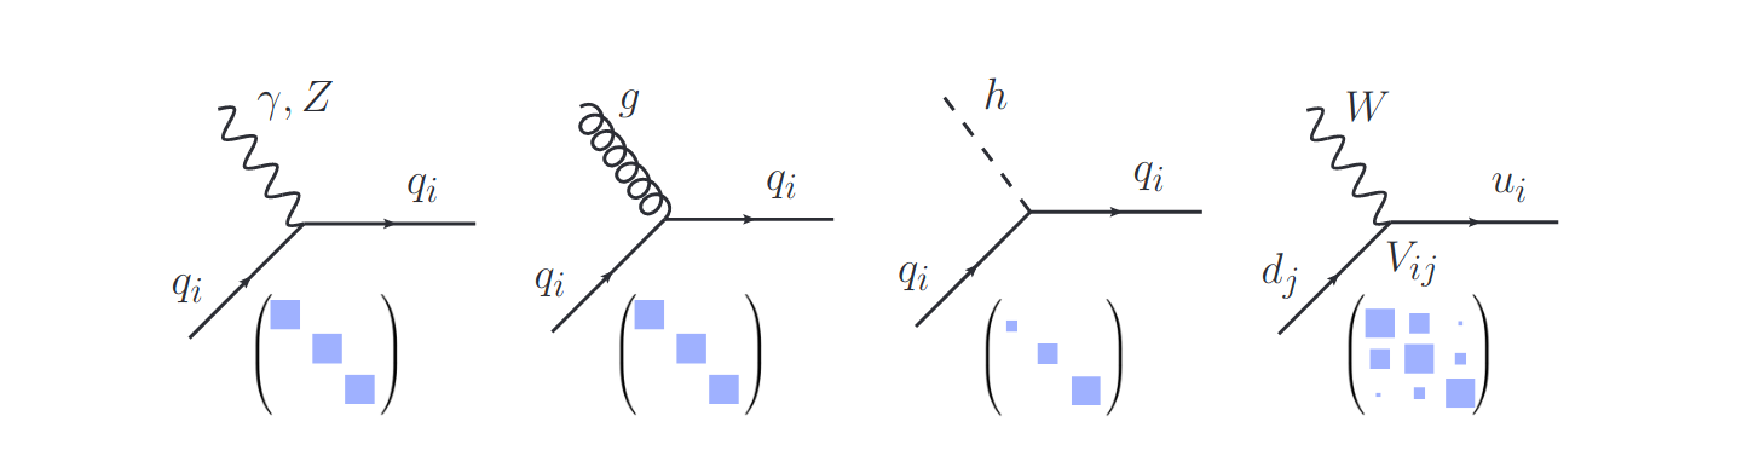
\includegraphics[width=1\textwidth]{TestYukawaCouplings.pdf}
	\caption{Feynman diagrams for flavour conserving couplings of quarks to photon, $Z$ boson, gluon and the Higgs (the first three diagrams), and the flavour changing coupling to the $W$ (the last diagram). The $3\times3$ matrices are visual representations of couplings in the generation space, with couplings to $\gamma$ ,$Z$, $g$ being flavour universal, while the couplings to the Higgs are flavour diagonal but not universal. Finally the couplings involving the $W$ are flavour changing and hierarchical.}
	\label{fig:QuarkCKM}
\end{figure}

In summary, the particle spectrum of the SM is composed by, the gauge bosons, $W^\pm$ and $Z$ bosons, mediators of the weak interactions, the photon $\gamma$, the electromagnetic interaction messenger and the strong force mediators, the gluons, $G$. Additionally, the model is also composed  by the matter particles, the fermions, composed by quarks and leptons. A spin-0 scalar also emerges known as the Higgs boson, $h$. 

Leptons and quarks are organized in three generations each, with 2 pairs by each generation leading to 6 different particles. For quarks we have the up and down for the first generation, charm and strange for the second as well as the top and bottom for the third one. Similarly, there are 6 types of leptons, the 3 charged leptons, electron, muon and tau, and the associated neutrinos. These are represented in different manners, being that the quarks are represented by $(u,d,c,s,t,b)$ while leptons as $(e,\nu_{e},\mu,\nu_{\mu},\tau,\nu_{\tau})$, where $\nu$ denotes the neutrinos. 

While quarks interact via the weak, electromagnetic and strong forces, the charged leptons only feel the electromagnetic and weak forces and the neutrinos are weakly interacting. 
%Grab-1 
After the process of SBB the charges (calculated through Eq.~(\ref{SM_Charge_Generator}) of the SM fields) read as seen in Tab.\,\ref{Table_Post_Break}.
%
\begin{table}[H]
	\caption{Quark and Lepton and charges after the process of SSB.}
	\centering
	\begin{tabular}{ccc}
		\hline & $\mathrm{SU(3)_C}$ & $\mathrm{U(1)_Q}$ \\
		\hline 
		Up type quarks $(u,c,t)$ & \textbf{3} & 2/3 \\
		Down type quarks $(d,s,b)$ & \textbf{3} & -1/3 \\
		Charged leptons $(e,\mu,\tau)$ & \textbf{1} & -1 \\
		Neutrinos  $(\nu_e,\nu_\mu,\nu_\tau)$  & \textbf{1} & 0 \\
		\hline	
	\end{tabular}
	\label{Table_Post_Break}
\end{table}
We can see that the last column in Tab.\,\ref{Table_Post_Break} stands for the electrical charge of each particle.


\section{Charged Flavour Currents vs. Neutral Flavor Currents}

It is noteworthy to highlight an important distinction between flavour changing neutral and charged currents. FCNCs are processes in which the quark flavour changes, but conserves its charge. The Flavour Changing Charged Currents (FCCCs) change both the flavour and the charge of the quark. This creates a important distinction between the two, seeing that FCCCs can involve up and down quarks, in the sense that a up quark can become a down quark, however this does not happen in FCNCs where we can only have a up or down sector quarks changing flavour to other up or down sector quarks. 

Extracting some representative probabilities from \cite{Tanabashi2018} reveals that the two types of processes are strikingly statistically different.  The charged currents lead to the dominant weak decays, while the FCNCs induce decays that are extremely suppressed. Rounding the experimental results, and not showing the errors, a few representative decays are seen in Tables\,\ref{Tab:Represent1} and \ref{Tab:Represent2}.
\setlength{\tabcolsep}{2pt} % Default value: 6pt
\renewcommand{\arraystretch}{1} % Default value: 1
%
\begin{table}[!hbt]
	%\caption{Global caption}
	\begin{minipage}{.5\linewidth}
		\caption{FCCCs examples}
		\label{Tab:Represent1}		
		\centering
		\begin{tabular}{lcl}
			$s \rightarrow u \mu^- \bar{\nu}_\mu $ & : & $\mathcal{BR}$ $\left( K^+ \rightarrow \mu^+ \bar{\nu} \right) = 64 \%$                 \\
			$b \rightarrow c \ell^- \nu_\ell $       & : &  $\mathcal{BR}$ $\left( B^- \rightarrow D^0 \ell \overline{\nu}_\ell \right) = 2.3 \% $ \\
			$c \rightarrow s \mu^\pm \nu_\mu $   & : &  $\mathcal{BR}$ $\left( D^\pm \rightarrow K^0 \mu^\pm \nu_\mu \right) = 9 \%$        
		\end{tabular}
	\end{minipage}%
	\begin{minipage}{.5\linewidth}
		\centering
		\caption{FCNCs examples}
		\label{Tab:Represent2}		
		\begin{tabular}{lcl}
			$s \rightarrow d \mu^+ \mu^- $ & : &  $\mathcal{BR}$ $\left( K_L \rightarrow\mu^+ \mu^- \right) =  7\times10^{-9}$        \\
			$ b \rightarrow d \mu^+ \mu^-$ & : &  $\mathcal{BR}$ $\left( B^- \rightarrow  K^{\** -} \ell^+ \ell^- \right) =  5\times10^{-7}$ \\
			$ c \rightarrow u \ell^+ \ell^-$     & : &  $\mathcal{BR}$ $\left( D^0 \rightarrow \pi \ell^+ \ell^- \right) =  1.8\times10^{-4}$      
		\end{tabular}
	\end{minipage} 
\end{table}

\setlength{\tabcolsep}{6pt} % Default value: 6pt
\renewcommand{\arraystretch}{1} % Default value: 1

The reason for such a striking difference is that in the SM the charged currents, as represented in Fig.\,\ref{fig:QuarkCKM}, occur at tree level, while FCNCs are forbidden at tree level and only arise starting at one loop order. Note the diagonal structure of neutral couplings (involving the $Z$ boson) for both the up and down families in Eq.~(\ref{LagFermFCCCs}). The relative complexity of FCNCs and FCCCs processes can be easily seen in Fig.~\ref{fig:Flavour_D_1}, where a 1-loop generated FCNC is illustrated next to a tree-level FCCC diagram.  
%
\begin{figure}[H]
\centering
\begin{minipage}{.09\textwidth}
    \ 
\end{minipage}
    \begin{minipage}{.40\textwidth}
        \large
        \begin{fmffile}{feyngraph_FCNCs_1}
        \begin{fmfgraph*}(110,60)
        \fmfleft{i2,i1}
        \fmfright{o2,o1}
        \fmf{fermion}{i2,v1,i1}
        \fmf{fermion}{o2,v2,o1}
        \fmf{boson,label=$W$,label.side=right,label.dist=10}{v2,v1}
        \fmflabel{$\ell^-$}{i1}
        \fmflabel{$\bar{\nu}_\ell$}{i2}
        \fmflabel{$\overline{\text{d}}_i$}{o2}
        \fmflabel{$u_j$}{o1}
        \end{fmfgraph*}
        \end{fmffile}
        \vspace{1em}
    \end{minipage}
    \begin{minipage}{.40\textwidth}
    \large
    \begin{fmffile}{feyngraph_FCNCs_2}
        \begin{fmfgraph*}(110,60)
        \fmfstraight
        \fmfleft{i1,i2}
        \fmfright{o1,o2}
        \fmf{fermion,tension=1}{i1,t1}
        \fmf{fermion,tension=1}{t2,i2}
        \fmf{boson,label=$W^+$,label.side=right,label.dist=10,tension=0.5}{t1,t4}
        \fmf{boson,label=$W^-$,label.side=left,label.dist=10,tension=0.5}{t2,t3}
        \fmf{fermion,label=$\nu_\ell$,label.side=left,tension=0.5}{t3,t4}
        \fmf{fermion,label={$\text{u} \comma c $},label.side=left,tension=0.5}{t1,t2}
        \fmf{fermion,tension=1}{t4,o1}
        \fmf{fermion,tension=1}{o2,t3}
        \fmflabel{$\bar{d},\bar{s}$}{i1}
        \fmflabel{$b$}{i2}
        \fmflabel{$\ell^+$}{o1}
        \fmflabel{$\ell^-$}{o2}
        \end{fmfgraph*}
    \end{fmffile}
    \end{minipage}
	\caption{Representative tree level charged current diagram (left) and a loop induced FCNC diagram (right).}
	\label{fig:Flavour_D_1}
\end{figure}
%
Furthermore, if one considers such loop contributions, the FCNCs are virtual processes and come suppressed by the difference of the quarks masses, $m^2_u-m^2_d$. This is the so called Glashow-Iliopoulos-Maiani (GIM) mechanism \cite{glashow1970weak}. Given the differences between the masses of the up and down sectors this has a significant impact.  
%
%%%

\subsubsection{Flavour as a Probe into New Physics}

Now that we have introduced a portion of flavor physics we can briefly touch on why collider experiments have been sold as a pathway to discovering new physics i.e.\,how deviation in rare decays could pin point exactly what is missing in the SM. 
%
Thanks to these large experiments we have many new observables in flavor physics, e.g. the branching ratios not coinciding with the SM prediction \cite{CasteloBranco2014} or observed Lepton Flavor Violation at tree and loop levels \cite{Graverini2019}. 
%
As well as providing limits on processes that are prohibited in the SM but that could happen in BSM contexts, such as lepton flavor violation in Higgs decays for models without Lepton flavour universality. 

However, one of the favored ways to search for NP is through FCNCs. 
%
This is because as mentioned there are no FCNCs at tree-level in the SM i.e.\,the gluon, Z and Higgs are strictly flavour conserving as we see in Fig.\,\ref{fig:QuarkCKM} at tree-level.
%
Thus, given that FCNC processes are heavily suppressed in the SM through the aforementioned GIM mechanism and their loop order, and seeing that FCNCs processes can be easily modified by NP, either through new tree level or loop level, contributions, these can serve as a good tool to search for exotic signatures. 

The recipe then, seems simple, identify processes that are rare in the SM and then search for deviations from the SM predictions and attempt to fit new physics as to explain these deviations. 
%
However, thus far all but a few processes are within $2\sigma$ experimental and theoretical bounds given by the SM.
%
Some of the most radical being the quark level transitions, $b \rightarrow s \mu \mu$ (See Ref. \cite{DAmico2017}) and $b \rightarrow c \tau \nu$ (See Ref. \cite{Hu2019}) channels.
%
These are, so far, showing over $ 4 \sigma$ deviations from their expected value. 

Without going into too much depth onto the NP searches, we can examine the scale at which these processes are "integrated out". 
%
This is the energy scale at which a NP operator would allow these processes to take place only at higher energies. These energies are naturally large and can be described as Eq.\,(\ref{eq:NP}). 
%
\bigbreak
%
\noindent
%
\begin{minipage}{.35\textwidth}
\begin{figure}[H]
	\label{fig:contactNP}
	\centering
	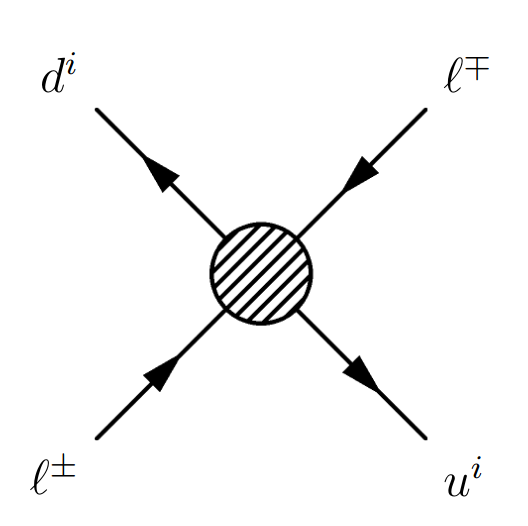
\includegraphics[width=0.6\textwidth]{My_First_Diagram.png}
	\caption{"Contact" interactions with loop interactions containing NP}
\end{figure}
\end{minipage}
\begin{minipage}{.6\textwidth}
	\begin{equation}
	\label{eq:NP}
	\mathcal{L}_{NP} \supset \frac{1}{\Lambda_{NP}} (\overline{Q}_i \gamma^\mu \sigma Q_j ) (\overline{L}_k \gamma_\mu \sigma L_l) ,  
	\end{equation}
\end{minipage}
%
\bigbreak
%
In particular, to explain $b \rightarrow s \mu \mu$ transitions we would need a $\Lambda_{NP} \approx 3 \ \text{TeV}$ while for $b \rightarrow c \tau \nu$ there would be the need of $\Lambda_{NP} \approx 30\ \text{TeV}$.
%
If confirmed, this would be an indicator for the need of NP, that would have to manifest at those energies-scales.

As for the FCNC diagram, the $b \rightarrow s \mu \mu$ channel can be seen in the top-left of Fig.~\ref{fig:Flavour_D_23_Muon}, while $b \rightarrow c \tau \nu$ flavour anomaly diagram can be seen in the top-right. These anomalies are very clean theoretically \cite{Fajfer_2012}. However, for the case of  $b \rightarrow c \tau \nu$ the NP effect in these diagrams is large ($\mathcal{O}(20\%)$) compared to the SM.
%
Consequently the NP interpretations here are often in conflict with experimental constraints. 
%
The theoretical bias here would have been that the new charged currents are either due to a charged Higgs, $H^+$ , or a new vector boson, $W^\prime$, see the bottom portions of Fig.\,\ref{fig:Flavour_D_23_Muon}. However these would have too large of an effect in the $B^-$ lifetime to fully explain the anomaly according to Ref.\,\cite{Alonso_2017} in most simple scenarios.
%
\begin{figure}[H]
\centering
    \begin{minipage}{.49\textwidth}
    \begin{fmffile}{decays_1}
        \begin{fmfgraph*}(120,120)
            \fmfstraight
            \fmfleft{x,g1,g2,x,s,dsleft,x}
            \fmfright{x,n1,n2,x,d,dsright,x}
            \fmfbottom{b}
            \fmflabel{$b$}{s}
            \fmflabel{$s$}{d}
            \fmf{fermion,tension=1}{s,v1}
            \fmf{fermion,tension=1}{v3,d}
            \fmf{photon,label=$W^-$,label.side=left,tension=1,foreground=(0.1,,0.1,,1)}{v1,v3}
            \fmf{fermion,label=$t$,right=0.4,tension=0.2,foreground=(0.1,,0.1,,1)}{v1,v2}
            \fmf{fermion,right=0.4,label.side=right,tension=0.2,foreground=(0.1,,0.1,,1)}{v2,v3}
            \fmf{phantom,tension=0.20}{v2,b}
            \fmf{photon,label=$\gamma \comma Z^0$,label.side=right,tension=0.5,foreground=(0.1,,0.1,,1)}{v2,v4}
            \fmf{fermion,tension=2}{n1,v4,n2}
            \fmf{phantom}{g1,v4,g2}
            \fmfv{label=$\mu^+$,label.angle=0}{n1}
            \fmfv{label=$\mu^-$,label.angle=0}{n2}
        \end{fmfgraph*}
    \end{fmffile}
    \end{minipage} \hspace{1em}
    \begin{minipage}{.30\textwidth}
        \large
        \begin{fmffile}{decays_pre}
        \begin{fmfgraph*}(120,60)
        \fmfleft{i3,i2,i1}
        \fmftop{t}
        \fmfright{o3,o2,o1}
        \fmf{fermion,tension=2.8}{i2,v1,t}
        \fmf{fermion}{o2,v2,o3}
        \fmf{boson,tension=0.1,label=$W^-$,label.side=left,tension=1,foreground=(0.1,,0.1,,1)}{v1,v2}
        \fmflabel{$\tau^-$}{o2}
        \fmflabel{$\bar{\nu}_\tau$}{o3}
        \fmflabel{$b$}{i2}
        \fmflabel{$c$}{t}
        \end{fmfgraph*}
        \end{fmffile}
    \end{minipage}
    \vspace{2em}
    \noindent\makebox[\linewidth]{\rule{\textwidth}{1pt}} 
    \begin{minipage}[t][0.1\textheight]{1\textwidth}
    \end{minipage}
	\vspace{1em}
    \begin{minipage}{.49\textwidth}
            \begin{fmffile}{decays_3}
            \begin{fmfgraph*}(120,60)
                        \fmfset{arrow_len}{10}
                        \fmfstraight
                        \fmfleft{i3,i1}
                        \fmfright{o3,o2,o1}
                        \fmf{fermion}{i1,v1,o1}
                        \fmffreeze
                        \fmf{fermion,tension=1.5}{o3,v3,o2}
                        \fmf{phantom,tension=1.8}{i3,v3}
                        \fmflabel{b}{i1}
                        \fmflabel{c\,(s)}{o1}
                        \fmflabel{$\tau$ ($\mu^-$)}{o2}
                        \fmflabel{$\nu_\tau$ ($\mu^+$)}{o3}
                        \fmf{boson,label=H$^\pm ,, (Z^{\prime},,H^0_{new})$,label.side=left,foreground=(1,,0.1,,0.1)}{v3,v1}
            \end{fmfgraph*}
        \end{fmffile}
    \end{minipage}
    \hspace{1em}
    \begin{minipage}{.30\textwidth}
        \large
        \begin{fmffile}{decays_4}
            \begin{fmfgraph*}(120,60)
                \fmfleft{i2,i1}
                \fmfright{o2,o1}
                \fmf{fermion}{i2,v1,i1}
                \fmf{fermion}{o2,v2,o1}
                \fmf{boson,label=LQ,label.side=right,label.dist=10,foreground=(1,,0.1,,0.1)}{v2,v1}
                \fmflabel{c(s)}{o1}
                \fmflabel{$\nu_\tau(\mu^+)$}{o2}
                \fmflabel{$b$}{i2}
                \fmflabel{$\tau^-(\mu^-)$}{i1}
            \end{fmfgraph*}
        \end{fmffile}
    \end{minipage}
    %
    \begin{minipage}[t][0.05\textheight]{1\textwidth}
    \end{minipage}
    \begin{minipage}{.3\textwidth}
        \begin{fmffile}{Decay_2222222222}
            \begin{fmfgraph*}(140,100)
                    \fmfstraight
                    \fmfleft{b,i1,t}
                    \fmftop{tt1,tt2,tt3,tt4}
                    \fmfright{o1,o2,o3,o4,o5}
                    \fmf{fermion,tension=1,label=$b$}{i1,v1}
                    \fmf{fermion,label=$t$,label.side=left,tension=1}{v1,v3}
                    \fmf{fermion,tension=1}{v3,o5}
                    \fmf{dashes,tension=0.4,foreground=(1,,0.1,,0.1),label=$H^+$,label.side=right}{v1,v2}
                    \fmf{dashes,tension=0.4,foreground=(1,,0.1,,0.1),label=$H^0$,label.side=right}{v2,v3}
                    \fmf{dashes,tension=1.5,label=$H^-$,foreground=(1,,0.1,,0.1)}{v2,v4}
                    \fmf{fermion,tension=1.5}{o1,v4}
                    \fmf{fermion}{v4,o3}
                    \fmflabel{$\nu_\tau$}{o3}
                    \fmflabel{$\tau^-$}{o1}
                    \fmflabel{$c$}{o5}
                    \end{fmfgraph*}
                \end{fmffile}
    \end{minipage}
    \vspace{1em}
	\caption{A set of representative SM diagrams that contribute towards $b \rightarrow s \mu \mu$ transition (left-top) and $b \rightarrow c \tau \nu$ transition (right-top). While in the lower mid section we find possible new NP contributions to $b \rightarrow c \tau \nu$ and $b \rightarrow s \mu \mu$ transition in brackets. In these diagrams, LQ, stands for a hypothetical Leptoquark particle that would interact with both leptons and quarks.  }
	\label{fig:Flavour_D_23_Muon}
\end{figure}
%
Another prediction of the SM is that the rates for the  $b \rightarrow s e^+ e^-$ and  $b \rightarrow s \mu^- \mu^+$ transitions should be equal to each other.
%
The SM prediction of Lepton Flavour Universality (LFU) is deeply ingrained in the structure of the theory, since it is a consequence of the fact that the electroweak gauge group is the same for all three generations. 
%
The prediction of LFU can be tested experimentally, also through flavour physics, by observables such as the ratio, 
%
\begin{equation}
R_{K^{\**}} = \frac{\text{Br}( B \rightarrow K^{\**} \mu^- \mu^+ )}{\text{Br} (  B \rightarrow K^{\**} e^- e^+  )} ,
\end{equation}
% 
Another possible hint of new physics is the fact the experimental value for this ratio is $R_{K^{\**}} \approx 0.7$, violating LFU by $2.2 - 2.6 \sigma$ \cite{Wei_2009}.  % Revealing to yet another discrepancy between the SM and reality. 
However, such a flavour anomaly will need to be studied at future runs of the LHC in order to collect more data, improve statistic and see whether the current anomaly vanishes away or else, if grows to a larger statistical significance. 
\endgroup

\chapter{B-L-SM Model} 
\label{Chap:B-L-SM_Model}
\begin{comment}

In this chapter we introduce the minimal $\U{B-L}$ gauge extension of the SM named, the B-L-SM Model \cite{Mohapatra:1980qe} and perform a numerical analysis as to measure how it can exist in light of modern measurements. This unitary group originates from the promotion of an accidental symmetry present in the SM, the Baryon number (B) minus the Lepton number (L) to a fundamental Abelian symmetry group, incidentally, also giving the model its name. Through this model we are capable of explaining the generation of neutrinos masses via a simple see-saw mechanism. This see-saw is enabled by the addition of three generations of right-handed heavy Majorana neutrinos that through the new field additions are possible free of anomalies. \cite{Yanagida:1979as}. Additionally, by virtue of two new physical states, specifically a new Higgs like boson $\mathrm{H}^\prime$ and a $\mathrm{Z}^\prime$ gauge boson we can also address other phenomenology, such as deviations in EW measurements, namely the $(g-2)_\mu$ anomaly \cite{Tanabashi2018}. The additional bosons acquire mass primarily through the spontaneous breaking of the $\U{B-L}$ symmetry that gives its name to the model. The energy scale of this breaking will also determine the mass scale for these bosons and heavy neutrinos. This (simple) mechanism for the mass generation of the referenced bosons means the model is already very heavily constrained due to long-standing direct searches at the LHC. 

Although a deceptively simple model it can be very appealing, as it benefits of many deep implications. Such as, through this model we can address the metastability of the EW vacuum in the SM through the new scalar. Allowing for Higgs stabilization up to the Plank scale with a new Higgs starting from a few hundred GeVs \cite{Degrassi:2012ry}. Metastability, simply put, is the thought to be observed, deeper minimum than the EW-VEV existing in the Higgs potential. This possibility deeply affects the formation of the early universe, especially during and after inflation making it a important question for cosmologists \cite{Ema_2017}. Note this is yet another phenomena that the SM cannot accommodate, further pointing at it only being accurate at low energy scales. The B-L-SM framework is also of particular interesting in the context of the study of Grand Unified Theories (GUT) as it easily embedded into higher order symmetry groups like the $\mathrm{SO(10)}$ \cite{Chanowitz:1977ye} or $\mathrm{E}_6$ \cite{Achiman:1978vg} Lie groups. Also, from these changes in the potential we can typically the enhanced strength of the EW phase transition potentially converting it into a strong first-order one. This could be detectable in the form of a gravitational wave background \cite{Barger:2008jx}. Such a analysis is of utmost importance given that it could provide a way to detect NP or exclude models without the need for a larger particle collider but instead novel gravitational waves experiments, such experiments are already planned in the form of LIGO or VIGO \cite{Abbott2020}. Furthermore, the existence of heavy neutrinos is also of cosmological significance given their presence could imply the existence of a sterile state that can play the role of Dark Matter \cite{Kaneta:2016vkq}, given that, the relatively small alteration of a, $\mathbb{Z}_2$, symmetry in the neutrino sector can make these fully sterile, as seen in Ref. \cite{Okada:2018ktp}. These neutrinos can, in such case, be used to help explain the baryon asymmetry via the leptogenesis mechanism, this scenario is discussed in depth in the following Refs.~\cite{Fukugita:1986hr}.

The B-L-SM contains a family-universal symmetry in the form of, $\mathrm{U(1)_{B-L}}$, if this symmetry was introduced without changing the SM fermion content this would lead to chiral anomalies i.e a non conservative charged current on some channels involving the $\mathrm{U(1)_{B-L}}$. These are not completely undesired by themselves, as they would allow for the presence of extra sources of $\mathcal{CP}$ violation, but this inclusion at tree-level without a suppression mechanism would lead to far too much $\mathcal{CP}$ violation. 

We structure this chapter in the following way, first, we present the fundamental theoretical background on the model with a strong focus on the basic details of the scalar and the gauge boson mass spectra and mixing. Followed by a modern precise study of the phenomenological status of the B-L-SM model through a layered algorithm that will be discussed preceding the results. With this algorithm we provide a numerical analysis that tests the relevant phenomenological constraints in direct and EW observables. We table off this chapter with a few representative benchmark points. 
\end{comment} 


\section{Introduction}
\label{sec:Introduction}

In this chapter we introduce the minimal $\U{B-L}$ gauge extension of the SM named, the B-L-SM Model  \cite{Basso:2011na} and perform a numerical analysis as to measure how it can exist in light of modern measurements. 

In the previous chapter we introduced many of the SMs flaws. 
%
One of which was the lack of a explanation of tiny neutrino masses confirmed by flavour-oscillation experiments. The minimal way of addressing this problem is by adding heavy Majorana neutrinos in order to realise a seesaw mechanism \cite{Mohapatra:1979ia}.
%
However, the mere introduction of an arbitrary number of heavy neutrino generations can raise new questions, in particular, how such a new scale is generated from a more fundamental theory. 

Among the simplest ultraviolet (UV) complete theories that dynamically addresses this question is the minimal gauge-$\U{B-L}$ extension of the SM, the B-L-SM model. 
%
As its name suggests, the B-L-SM promotes an accidental conservation of the difference between baryon (B) and lepton (L) numbers in the SM to a fundamental local Abelian symmetry group.
%
Furthermore, such a $\U{B-L}$ symmetry can be embedded into larger groups such as e.g.~$\SO{10}{}$ \cite{Chanowitz:1977ye} %,Georgi:1978fu,Georgi:1979dq,Georgi:1979ga}
 or $\E{6}$ \cite{Achiman:1978vg}%,Gursey:1981kf}
, making the B-L-SM model well motivated by Grand Unified Theories (GUTs).
%
The presence of three generations of right-handed neutrinos also ensures a framework free of anomalies with their mass scale developed once the $\U{B-L}$ is broken by the VEV of a complex SM-singlet scalar field, simultaneously giving mass to the corresponding $Z^\prime$ boson.

The cosmological implications of the B-L-SM are also relevant. First, the presence of an extended neutrino sector implies the existence of a sterile state that can play a role of $\ro{keV}$- to $\ro{TeV}$-scale Dark Matter candidate \cite{Kaneta:2016vkq}. 
%
Particularly, it can be stabilized by imposing a $\mathbb{Z}_2$ parity as it was done e.g.~in Refs.~\cite{Okada:2018ktp}. 
%
The $\U{B-L}$ model with sterile neutrino Dark Matter can also explain the observed baryon asymmetry via the leptogenesis mechanism (see Refs.~\cite{Dev:2017xry}, for details).
%
As was mentioned earlier, the B-L-SM features an extended scalar sector with a complex SM-singlet state $\chi$ which, besides enriching the Higgs sector with a new potentially visible state, can cure the well-known metastability of the electroweak (EW) vacuum in the SM \cite{Buttazzo:2013uya}.
%
Indeed, it was shown in Ref.~\cite{Costa:2014qga} that an additional physical scalar with a mass beyond a few hundred $\ro{GeV}$ can stabilize the Higgs vacuum all the way up to the Plank scale. In the framework of B-L-SM, a complete study of the scalar sector was performed in Ref.~\cite{Basso:2010jm} where the vacuum stability conditions valid at any renormalization group scale were derived. Last, but not least, the presence of the complex SM-singlet $\chi$ interacting with a Higgs doublet typically enhances the strength of EW phase transition potentially converting it into a strong first-order one \cite{Barger:2008jx}.

Another open question that finds no solution in the SM is the discrepancy between the measured anomalous magnetic moment of the muon, $a_\mu^{\ro{exp}} \equiv {1}/{2} \left(g-2\right)^{\ro{exp}}_\mu$, and its theoretical prediction, $a_\mu^{\ro{SM}} \equiv {1}/{2} \left(g-2\right)^{\ro{SM}}_\mu$, which reads \cite{Tanabashi:2018oca,Zyla}
\begin{equation}
\label{g-2}
\Delta a_\mu = a_\mu^{\ro{exp}} - a_\mu^{\ro{SM}} = 268(63)(43) \times 10^{-11}
\end{equation}
with numbers in brackets denoting experimental and theoretical errors, respectively. This represents a tension of $3.5$ standard deviations from the combined $1 \sigma$ error and is calling for new physics effects beyond the SM theory. In a recent work \cite{Campanario:2019mjh} it was further claimed that SM higher order perturbative corrections cannot explain $\Delta a_\mu$. 
%
Radiative corrections with new gauge bosons can enhance the theoretical value of the muon anomaly such that \eqref{g-2} is satisfied \cite{Czarnecki:2001pv}. This is indeed the case of the B-L-SM, or its SUSY version \cite{Yang:2018guw}, where a new $Z^\prime$ gauge boson can explain $\Delta a_\mu$. 

In a recent work \cite{Deppisch:2019ldi}, the impact of LHC searches for a light $Z^\prime$ boson, i.e.~with mass in the range of $0.2~\ro{GeV}$ to $200~\ro{GeV}$, was thoroughly investigated. 
%
The current collider bounds are available from the ATLAS  \cite{Aad:2019fac} and CMS \cite{Sirunyan:2018exx} searches for Drell-Yan $Z^\prime$ production decaying into di-leptons, 
i.e.~$pp \to Z^\prime \to ee,\mu \mu$. In the current work, we perform a complementary study where, for heavy (TeV-scale) $Z^\prime$ masses, the combined effect of the electroweak precision and Higgs observables and collider constraints on the $pp \to Z^\prime \to ee,\mu \mu$ channel, is investigated. We analyse whether the existing LHC constraints leave any room for partially explaining the $(g-2)_\mu$ anomaly and which impact it has on the model parameters and other physical observables such as the $\U{B-L}$ gauge coupling $\g{B-L}{}$, the kinetic mixing parameter $\g{YB}{}$ and the extra scalar and $Z^\prime$ boson masses. Furthermore, with the current Muon $(g-2)_\mu$ experiment E989 at Fermilab \cite{Grange:2015fou}, it will be possible to either confirm or eliminate, at least partially, the currently observed discrepancy.

This chapter is organized as follows, in Section~\ref{sec:BLSM}, we give a brief description of the B-L-SM structure focusing on the basic details of scalar and gauge boson mass spectra and mixing. In Section~\ref{sec:parameter-space-studies}, a detailed discussion of the numerical analysis is provided. In particular, we outline the methods and tools used in our numerical scans as well as the most relevant phenomenological constraints leading to a selection of a few representative benchmark points. Besides, the numerical results for correlations of the $Z^\prime$ production cross section times its branching ratio into light leptons versus the model parameters and the muon $(g-2)_\mu$ are presented. 

\section{Formulating the Model}
\label{sec:BLSM}

In this section, we highlight the essential features of the minimal $\U{B-L}$ extension of the SM relevant for our analysis. Essentially, the minimal B-L-SM is a BSM framework containing three new ingredients, a new gauge interaction given the new symmetry group, three generations of right handed neutrinos, and a complex scalar field $\chi$. 
%
The first of these is well motivated in various GUT scenarios.
%
However, if a family-universal symmetry such as $\U{B-L}$ were introduced without changing the SM fermion content, chiral anomalies involving the $\U{B-L}$ external legs would be generated. A new sector of additional three $B-L$ charged Majorana neutrinos is essential for anomaly cancellation. Also, the SM-like Higgs doublet, $H$, does not carry neither baryon nor lepton number, therefore does not participate in the breaking of $\U{B-L}$. It is then necessary to introduce a new scalar singlet, $\chi$, solely charged under $\U{B-L}$, whose VEV breaks the $B-L$ symmetry at a scale $\mean{\chi} > \mean{H}$. It is also this breaking scale that generates masses for heavy neutrinos. The particle content and charges of the minimal $\U{B-L}$ extension of the SM are summarized in Tab.~\ref{tab:BLSM_Charges}.

\begin{table}[H]
	\centering
	\begin{tabular}{|c|c|c|c|c|c|c|c|c|}
		\hline
		& $q_L$  & $u_R$ & $d_R$ & $l_L$  & $e_R$ & $\nu_R$  &  $H$  & $\chi$  \\ \hline
		$\mathrm{SU(3)_C}$& $\mathbf{3}$ & $\mathbf{3}$  & $\mathbf{3}$  & $\mathbf{1}$  & $\mathbf{1}$   & $\mathbf{1}$   & $\mathbf{1}$    & $\mathbf{1}$    \\
		$\mathrm{SU(2)_L}$& $\mathbf{2}$  & $\mathbf{1}$ & $\mathbf{1}$ & $\mathbf{2}$ & $\mathbf{1}$ & $\mathbf{1}$ & $\mathbf{2}$  & $\mathbf{1}$ \\
		$\mathrm{U(1)_Y}$ & ${1}/{6}$ & ${2}/{3}$  & -${1}/{3}$  & -${1}/{2}$ & -1 & 0 & ${1}/{2}$ & 0 \\
		$\mathrm{U(1)_{B-L}}$ & ${1}/{3}$ & ${1}/{3}$ & ${1}/{3}$  & -1  & -1 &-1  & 0 & 2  \\ \hline 
	\end{tabular}
	\caption{Quantum fields and their respective quantum numbers in the minimal B-L-SM extension. The last two lines represent the weak and $B-L$ hypercharges}
	\label{tab:BLSM_Charges}
\end{table} 

\subsection{Scalar sector}

Given the information presented in Tab.~\ref{tab:BLSM_Charges} we can now construct all the Lagrangian terms for this theory. Much of which would be similar to the SM - we will however focus on the novel terms. We begin our study of NP in the B-L-SM by presenting the new scalar potential, which now includes two fields and reads, 
%
\begin{equation}
\label{eq:potential}
V(H,\chi) = \mu_1^2 H^\dagger H + \mu_2^2 \chi^\ast \chi + \lambda_1 (H^\dagger H)^2 + \lambda_2 \left(\chi^\ast \chi\right)^2 + \lambda_3  \chi^\ast \chi H^\dagger H \ , 
\end{equation}
%
where,  $\lambda_i$, the scalar couplings and $\mu_{1,2}^2$ the quadratic terms for $H$ and $\chi$ respectively, with $v$ and $x$ are the vacuum expectation values (\vevs) describing the classical ground state configurations for the same fields. The full components of the scalar fields $H$ and $\chi$ are given by,
%
\begin{equation}
H = \frac{1}{\sqrt{2}} 
\begin{pmatrix}
 \omega_1 + i \omega_2  \\
v + (h + i z)
\end{pmatrix} \quad , ~\quad \chi = \frac{1}{\sqrt{2}} \left( x + \left(h^\prime + i z^\prime\right) \right) , 
\end{equation}
%
There are four Goldstone directions denoted as $\omega_1$, $\omega_2$, $z$ and $z^\prime$ which are absorbed into longitudinal modes of the $W$, $Z$ and $Z^\prime$ gauge bosons once SBB takes place.

This potential in Eq.~(\ref{eq:potential}) must lead to a stable vacuum state, which means that the scalar potential must be bounded from below (BFB), i.e ensure a global minima. Such conditions can be deduced by evaluating its derivatives and finding null conditions, these are commonly called tadpole equations. These conditions are seen in Eq.~(\ref{eq:BFB}) (shown in \cite{Basso:2010jm}).
%
\begin{equation}
4 \lambda_1 \lambda_2  -  \lambda_3^2 > 0 \quad , \quad \lambda_1 , \lambda_2>0 
\label{eq:BFB} \ .
\end{equation}
%
If these conditions are satisfied the electric charge conserving vacuum takes the form of,
\begin{equation}
\mean{H} = \dfrac{1}{\sqrt{2}} 
\begin{pmatrix}
0 \\
v 
\end{pmatrix}	
\qquad
\mean{\chi} = \dfrac{x}{\sqrt{2}}
\label{eq:vacuum}
\end{equation}
%
In these equations we can see that $h$ and $h^\prime$ represent the radial quantum fluctuations around the minimum of the potential.
%
These will constitute the physical degrees of freedom associated with $H$ and $H^\prime$. There are also four Goldstone directions denoted as $\omega_1$, $\omega_2$, $z$ and $z^\prime$ which are absorbed into longitudinal modes of the $W^\pm$, $Z$ and $Z^\prime$ gauge bosons once SSB takes place. 
 
The tadpole equations can be solved in order to each of the VEVs, returning the following Eqs.,
%
\begin{equation}
v^2 = \tfrac{-\lambda_2 \mu_1^2 + \tfrac{\lambda_3}{2}\mu_2^2}{\lambda_1 \lambda_2 - \tfrac{1}{4}\lambda_3^2} > 0
\qquad
\text{and}
\qquad
x^2 = \tfrac{-\lambda_1 \mu_2^2 + \tfrac{\lambda_3}{2}\mu_1^2}{\lambda_1 \lambda_2 - \tfrac{1}{4}\lambda_3^2} > 0 , 
\label{eq:extremum}
\end{equation}
%
which, when simplified with the BFB conditions yield a simpler set of equations,
%
\begin{equation}
\lambda_2 \mu_1^2 < \tfrac{\lambda_3}{2} \mu_2^2 
\qquad
\text{and}
\qquad
\lambda_1 \mu_2^2 < \tfrac{\lambda_3}{2} \mu_1^2 \ . 
\label{eq:sols}
\end{equation}
%
Note that although $\lambda_1$ and $\lambda_2$ must be positive to ensure the correct conical shape of the potential, no such conditions exist for the sign of $\lambda_3$ , $\mu_1$, and $\mu_2$. However observing Eq\,(\ref{eq:sols}) we can infer that only some combinations of signs are impossible, 
%
\begin{table}[!htb]
	\begin{center}
		\begin{tabular}{ccccc}
			& $\mu_2^2 > 0$ & $\mu_2^2 > 0$ & $\mu_2^2 < 0$ & $\mu_2^2 < 0$  	\\
			& $\mu_1^2 > 0$ & $\mu_1^2 < 0$ & $\mu_1^2 > 0$ & $\mu_1^2 < 0$  	\\        
			\hline  
			$\lambda_3 < 0 $     			    							& 	\xmark		& \checkmark	&	\checkmark & \checkmark	\\
			$\lambda_3 > 0$     			    							& \xmark		& \xmark	&	\xmark &  \checkmark \\
			\hline
		\end{tabular} 
		\caption{Possible signs of the potential parameters in Eq\,(\ref{eq:potential}). 
			The \checkmark\,symbol indicates the existence of solutions for tadpole conditions Eq.\,\eqref{eq:sols}, while the \xmark\,indicates unstable configurations.}
		\label{tab:signs}  
	\end{center}
\end{table} 
%
For our numerical analysis we decided to leave the sign of $\lambda_3$ positive, choosing a configuration where both $\mu$ parameters are negative. 
%
This does not directly translate to any real physical consequence.

With these conditions now established we proceed to investigate the physical states of the B-L-SM scalar sector. 
%
At the vacuum, we evaluate the Hessian matrix as,
%´
\begin{equation}
\mathbf{M}^2 =
\begin{pmatrix}
4 \lambda_2 x^2 & \lambda_3 v x \\ 
\lambda_3 v x   & 4 \lambda_1 v^2 
\end{pmatrix}\,.
\label{eq:hess}
\end{equation}
% 
Moving this matrix to its physical mass eigenbase, we obtain the following eigenvalues,
%
\begin{equation}
m_{h_{1,2}}^2 = \lambda_1 v^2 + \lambda_2 x^2 \mp \sqrt{(\lambda_1 v^2 - \lambda_2 x^2)^2 + (\lambda_3 x v)^2}.
\label{eq:eigvals}
\end{equation} 
%
The physical basis vectors $h_1$ and $h_2$ can then be related to the original fields of gauge eigenbasis $h$ and $h^\prime$ through a simple rotation matrix:
%
\begin{equation}
\begin{pmatrix}
h_1 \\
h_2 
\end{pmatrix}
=
\mathbf{O}
\begin{pmatrix}
h \\
h^\prime 
\end{pmatrix},
\label{eq:trans}
\end{equation}
%
where $\mathbf{O}$ can be parameterized by a single mixing angle $\alpha_h$,
%
\begin{equation}
\mathbf{O} = 
\begin{pmatrix}
\cos \alpha_h & -\sin \alpha_h \\
\sin \alpha_h & \cos \alpha_h 
\end{pmatrix}\,.
\label{eq:rotmat}
\end{equation}
%
It is particularly interesting to analyze the scenario where the scalar fields approximately decouple, that is, in the limit, $v/x\ll 1$. In these circumstances, the scalar masses and the mixing angle become rather simple,
\begin{equation}
\sin \alpha_h \approx \dfrac{1}{2}\dfrac{\lambda_3}{\lambda_2} \dfrac{v}{x} \quad , \quad 
m_{h_1}^2 \approx 2 \lambda_1 v^2 \quad , \quad m_{h_2}^2 \approx 2 \lambda_2 x^2
\label{eq:simplify} .
\end{equation}

\subsection{Gauge Sector}

Moving onto the gauge boson and Higgs kinetic terms in the B-L-SM, consider the following section of the Lagrangian,
\begin{equation}
\mathcal{L}_{\mathrm{U(1)'s}} =  \left| D_\mu H \right|^2 + \left| D_\mu \chi \right|^2 -\dfrac{1}{4} F_{\mu \nu} F^{\mu \nu} -\dfrac{1}{4} F^\prime_{\mu \nu} F^{\prime \mu \nu} -\dfrac{1}{2} \kappa F_{\mu \nu} F^{\prime \mu \nu} , 
\label{eq:Lu1}
\end{equation}
where $F^{\mu \nu}$ and $F^{\prime \mu \nu}$ are the standard field strength tensors, respectively for the $\U{Y}$ and  $\U{B-L}$ Abelian groups, 
\begin{equation}
F_{\mu \nu} = \partial_\mu A_\nu - \partial_\nu A_\mu 
\qquad
\text{and}
\qquad
F^\prime_{\mu \nu} = \partial_\mu A^\prime_\nu - \partial_\nu A^\prime_\mu\,,
\label{eq:Fmn}
\end{equation}
written in terms of the gauge fields $A_\mu$ and $A_\mu^\prime$, respectively. Given that this is a model with two Unitary groups, without a parity symmetry ($\mathbb{Z}_2$) to prevent it, we must consider the possible mixing in between them. In this work we parameterized this mixing through a parameter $\kappa$.

With this goal in mind consider the Abelian terms of the covariant derivative in Eq.\,(\ref{eq:Lu1}) is given by,
\begin{equation}
D_\mu \supset i g_1 Y A_\mu + i g_1^\prime Y_{\rm B-L} A_\mu^\prime\,,
\end{equation} 
% 
with $g_1$ and $g_1^\prime$ the $\U{Y}$ and $\U{B-L}$ the gauge couplings with the $Y$ and $B-L$ charges are specified in Tab.~\ref{tab:BLSM_Charges}. It is convenient to rewrite the gauge kinetic terms in the canonical form, i.e.
%
\begin{equation}
F_{\mu \nu} F^{\mu \nu} + F^\prime_{\mu \nu} F^{\prime \mu \nu} + 2 \kappa F_{\mu \nu} F^{\prime \mu \nu} \to B_{\mu \nu} B^{\mu \nu} + B^\prime_{\mu \nu} B^{\prime \mu \nu}\,.
\label{eq:AtoB}
\end{equation}
%
A generic orthogonal transformation in the field space does not eliminate the kinetic mixing term. So, in order to satisfy Eq.~\eqref{eq:AtoB} an extra non-orthogonal transformation should be imposed such that Eq.~\eqref{eq:AtoB} is realized. Taking $\kappa = \sin \alpha$, a suitable redefinition of fields $\{A_\mu,A_\mu^\prime\}$ into $\{B_\mu, B_\mu^\prime\}$ that eliminates $\kappa$-term according to Eq.~\eqref{eq:Lu1} can be cast as
\begin{equation}
\begin{pmatrix}
A_\mu \\
A^\prime_\mu 
\end{pmatrix}
=
\begin{pmatrix}
1 & -\tan \alpha \\
0 & \sec \alpha 
\end{pmatrix}
\begin{pmatrix}
B_\mu \\
B^\prime_\mu 
\end{pmatrix}\,.
\label{eq:trans-kappa}
\end{equation}
Note there is a limit without kinetic mixing where $\alpha = 0$. Note that this transformation is generic and valid for any basis in the field space. The transformation (\ref{eq:trans-kappa}) results in a modification of the covariant derivative that acquires two additional terms encoding the details of the kinetic mixing, i.e.

\begin{equation}
D_\mu \supset \partial_\mu + i \left(g_Y \; Y + g_BY \; Y_{B-L}\right) B_\mu + i \left(g_{B-L} \; Y_{B-L} + g_{YB} \; Y\right) B_\mu^\prime\,,
\label{eq:newCov}
\end{equation}	
where the gauge couplings take the form
\begin{equation}
g_Y = g_1 \quad , \quad 
g_{B-L} = g_1^\prime \sec \alpha   \quad , \quad 
g_{YB} = -g_1 \tan \alpha  \quad , \quad 
g_{BY} = 0 \,,  
\label{eq:new-g-simp}
\end{equation}
%
which is the standard convention in the literature.
%
Note that this definition is merely to simplify the equations and has no physical impact. 
%
We will later see that this kinetic mixing is a desired feature and why stabilizing it with a $\mathbb{Z}_2$ symmetry would be detrimental in terms of depth.
%
The resulting mixing between the neutral gauge fields including $Z^\prime$ can be represented as follows
%
\begin{equation}
\begin{aligned}
\begin{pmatrix}
\gamma_\mu \\
Z_\mu \\
Z^\prime_\mu
\end{pmatrix}
=
\begin{pmatrix}
\cos \theta_W & \sin \theta_W & 0\\
-\sin \theta_W \cos \theta_W^\prime & \cos \theta_W \cos \theta_W^\prime & \sin \theta_W^\prime \\
\sin \theta_W \sin \theta_W^\prime & -\cos \theta_W^\prime \sin \theta_W^\prime & \cos \theta_W^\prime
\end{pmatrix}
\begin{pmatrix}
B_\mu \\
A^3_\mu \\
B^\prime_\mu
\end{pmatrix} , 
\end{aligned}
\label{eq:g-Z-Zp}
\end{equation}
%
where $\theta_W$ is the weak mixing angle and $\theta^\prime_W$ is defined as
\begin{equation}
\sin(2 \theta^\prime_W) = \frac{2 g_{YB} \sqrt{g^2 + g_{Y}^2}}{\sqrt{(g_{YB}^2 + 16 (\frac{x}{v})^2 g_{B-L}^2 - g^2 - g_{Y}^2)^2 + 4 g_{YB}^2 (g^2 + g_{Y}^2)} }\,,
\label{eq:theta-p-full}
\end{equation}
%
in terms of $g$ and $g_{Y}$ being the $\mathrm{SU(2)_{L}}$ and $\mathrm{U_{Y}}$ gauge couplings, respectively. In the physically relevant limit, $v/x \ll 1$, the above expression greatly simplifies leading to
%
\begin{equation}
\sin \theta_W^\prime \approx \dfrac{1}{16
} \dfrac{g_{YB}}{g_{B-L}}\left( \dfrac{v}{x} \right)^2 \sqrt{g^2 + g_{Y}^2} \,,
\label{eq:theta-p}
\end{equation}
%
up to $(v/x)^3$ corrections. In the limit of no kinetic mixing, i.e. $g_{YB} \to 0$, there is no mixture of $Z^\prime$ and SM gauge bosons. 

Note, that the kinetic mixing parameter $\theta_W^\prime$ has rather stringent constraints from $Z$ pole experiments both at the Large Electron-Positron Collider (LEP) and the Stanford Linear Collider (SLC), restricting its value to be smaller than $10^{-3}$ approximately \cite{Bandyopadhyay_2018}, which we set as an upper bound in our numerical analysis. 

Finally we can, through the expansion of the kinetic terms $\left| D_\mu H \right|^2 + \left| D_\mu \chi \right|^2$ around the vacuum, extract the following mass matrix for the vector bosons
\begin{equation}
m_V^2 =
\dfrac{v^2}{4}
\begin{pmatrix}
g^2 \;\;&\;\; 0 \;\;&\;\; 0 \;\;&\;\; 0 \;\;&\;\; 0 \\
0 \;\;&\;\; g^2 \;\;&\;\; 0 \;\;&\;\; 0 \;\;&\;\; 0 \\
0 \;\;&\;\; 0 \;\;&\;\; g^2 \;\;&\;\; -g g_{Y} \;\;&\;\; -g g_{YB} \\
0 \;\;&\;\; 0 \;\;&\;\; -g g_{Y} \;\;&\;\; g_{Y}^2 \;\;&\;\; g_{Y} g_{YB} \\
0 \;\;&\;\; 0 \;\;&\;\; -g g_{YB} \;\;&\;\; g_{Y} g_{YB} \;\;&\;\; g_{YB}^2 + 16 \left(\dfrac{x}{v}\right)^2 g_{B-L}^2
\end{pmatrix} , 
\end{equation}
%
whose, first set of eigenvalues read,
\begin{equation}
m_A = 0 \quad \text{,} \quad m_{W^\pm} = \tfrac{1}{2} v g \ , 
\end{equation}
corresponding to the expected physical photon and $W^\pm$ bosons. While the following set,
\begin{equation}
m_{Z,Z^\prime}=\sqrt{g^2 + g^2_{Y}} \cdot \frac{v}{2}  \sqrt{\frac{1}{2} \left( \frac{g_{YB}^2 + 16 (\frac{x}{v})^2 g^2_{\rm BL} }{g^2 + g^2_{\rm Y}} +1  \right) \mp \frac{g_{YB}}{\sin(2 \theta_W^\prime) \sqrt{g^2 + g^2_{\rm Y}}}}\,,
\label{eq:ZZp-mass}
\end{equation}
correspond to two neutral massive vector bosons, with one of them, not necessarily the lightest, representing the SM-like $Z$ boson. It follows from LEP and SLC constraints on $\theta_W^\prime$, that Eq.~\eqref{eq:theta-p} also implies that either $g_{YB}$ or the ratio ${v}/{x}$ are small. In this limit, Eq.~\eqref{eq:ZZp-mass} simplifies to
\begin{equation}
m_Z \approx \tfrac{1}{2} v \sqrt{g^2 + g_{Y}^2} \qquad \text{and} \qquad m_{Z^\prime} \approx 2 g_{B-L} x\,,
\label{eq:mZ}
\end{equation}
%
where the $m_{Z^\prime}$ depends only on the SM-singlet VEV ,$x$ and on the $\mathrm{U(1)_{B-L}}$ gauge coupling and will be attributed to a heavy $Z^\prime$ state, while the light $Z$-boson mass corresponds to its SM value.

\subsection{The Yukawa Sector}

One of the key features of the B-L-SM model is the presence of non-zero neutrino masses. 
%
In its minimal version, such masses are generated via a type-I seesaw mechanism, thus producing a very light neutrino for each of the three known flavors, and a corresponding heavy neutrino one for each, which we theorize are yet to be observed.
%
In the type-I seesaw mechanism the mixing of neutrinos fields is written with similar shape to, 
\begin{equation}
\left( \begin{array}{c|c}
0 & A \\
\midrule
A & B 
\end{array} \right) . 
\end{equation}
This system would have a set eigenvalues written as, 
\begin{equation}
\lambda_\pm = \frac{ B \pm \sqrt{B^2 + 4 A} }{ 2 } \ . 
\end{equation}
Investigating the nature of these eigenvalues allows us to understand the see-saw process.
%
The mean of these values being always equal to $|B|$, if one value goes up, another goes down, like a see-saw. $B$ is set to be proportional to Majorana mass terms, orders of magnitude higher than the cross-terms $A$. Given this, the smaller eigenvalue, is, 
\begin{equation}
\lambda_- \approx \frac{A^2}{B} . 
\end{equation}
This mechanism serves to explain why the neutrino masses are so small if there exists a much heavier partner in the see-saw. 

The total Yukawa Lagrangian of the model reads,
\begin{equation}
\begin{aligned}
\mathcal{L}_f = 
-Y_u^{ij} \bar{q}_{\rm L i} u_{\rm R j} \widetilde{H} 
-Y_d^{ij} \bar{q}_{\rm L i} d_{\rm R j} H
-Y_e^{ij} \bar{\ell}_{\rm L i} e_{\rm R j} H
- Y_\nu^{ij} \bar{\ell}_{\rm L i} \nu_{\rm R j} \widetilde{H}
-\dfrac{1}{2} Y_\chi^{ij} \overline{\nu}_{\rm R i}^c \nu_{\rm R j} \chi + {\rm H.c.} \ . 
\end{aligned}
\label{eq:Yuk}
\end{equation}
%
Notice the explicit lack of Majorana neutrino mass terms of the form $M \overline{\nu_{R}^c} \nu_{R}$. 
These explicitly violate the $\mathrm{U(1)_{B-L}}$ symmetry and are therefore not present. 
In Eq.~\eqref{eq:Yuk}, $Y_u$, $Y_d$ and $Y_e$ are the $3 \times 3$ Yukawa matrices that reproduce the quark and charged lepton sector exactly the same way as in the SM, while $Y_\nu$ and $Y_\chi$ are the new Yukawa matrices responsible for the generation of right handed neutrino masses and mixing with left handed fields.
%
In particular, one can write,
\begin{equation}
\mathbf{m}_{\nu_l}^{\text{Type-I}} = \dfrac{1}{\sqrt{2}}\dfrac{v^2}{x} \mathbf{Y}_\nu^t \mathbf{Y}^{-1}_\chi \mathbf{Y}_\nu\,,
\end{equation}
%
for light $\nu_l$ neutrino masses, whereas the heavy $\nu_h$ ones are given by
\begin{equation}
\mathbf{m}_{\nu_h}^{\text{Type-I}} \approx \dfrac{1}{\sqrt{2}} \mathbf{Y}_\chi x\,,
\end{equation} 
where we have assumed a flavor diagonal basis.

Note that the smallness of light neutrino masses imply that either the $x$ VEV is very large or (if we fix it to be at the $\mathcal{O}\left({\mathrm{TeV}}\right)$ scale and $\mathbf{Y}_\chi \sim \mathcal{O}\left(1\right)$) the corresponding Yukawa coupling should be tiny, $\mathbf{Y}_\nu < 10^{-6}$. 
%
It is clear that the low scale character of the type-I seesaw mechanism in the minimal B-L-SM is \textit{faked} by small Yukawa couplings to the Higgs boson. A more elegant description was proposed in Ref.~\cite{Khalil:2010iu} where small SM neutrino masses naturally result from an inverse seesaw mechanism.
%
In this work, however, we will not study the neutrino sector and thus, for an improved efficiency of our numerical analysis of $Z^\prime$ observables, it will be sufficient to fix the Yukawa couplings to $\mathbf{Y}_\chi = 10^{-1}$ and $\mathbf{Y}_\nu = 10^{-7}$ values such that the three lightest neutrinos lie in the sub-eV domain.


\section{Numerical Results}
\label{sec:parameter-space-studies}

The numerical data presented in this section was generated via a large chain of nested scripts. These were created as a first generation of a scanning framework for generic phenomenological models. This machinery was  later adapted to the case of the 3HDM discussed in chapter \ref{ch:3HDM}. 

The underlying code is a mixture of Linux bash and Python3 scripts, and utilizes \texttt{SPheno 4.0.3} \cite{Porod:2011nf},  \texttt{SARAH 4.13.0} \cite{Staub:2013tta}, \texttt{HiggsBounds 4.3.1} \cite{Bechtle:2013wla}, \texttt{HiggsSignals 1.4.0} \cite{Bechtle:2013xfa} and \texttt{MadGraph5\_aMC@NLO 2.6.2} \cite{Alwall:2014hca} programs/packages. 

These scripts generate a logarithmic Monte-Carlo-like scan through a desired parameter space. Unless introduced, all non-relevant physical constants and parameters are defined in a way as to keep the observed gauge, lepton and quark structure consistent with real measurements. 
%
The points that fail this initial check must be rejected before even considering experimental constraints. This is done automatically by \texttt{SPheno}, which is a spectrum generator that calculates all necessary observables. \texttt{SPheno} takes all the required information about the model structure from \texttt{SARAH 4.13.0} and creates an executable that automatically generates a spectrum file in the SUSY Les Houches Accord (SLHA) \cite{Skands:2003cj} format. In our routine, each sampled point generates a SLHA file that is processed and stored. 
%
The second layer of tests includes the phenomenological studies we shall perform. This is where we confront the surviving scenarios with experimental data such as precision measurements from the oblique $S,T,U$ parameters and constraining the Higgs sector such that it agrees with both the observed signal seen at the LHC, and exclusions limits from new scalar direct searches. The latter is made automatically through the package \texttt{HiggsBounds 4.3.1} that shall be used to apply a $95\%$ C.L. exclusion limit cut on a new scalar particle, $h_2$, while \texttt{HiggsSignals 1.4.0} is used to calculate and later check, through a $\chi^2$ distribution, the probability for consistency with the observed Higgs boson signal data. To calculate these variables \texttt{HiggsBounds 4.3.1} and \texttt{HiggsSignals 1.4.0} need all scalar masses, total decay widths, Higgs decay branching ratios as well as the SM-normalized effective Higgs couplings to fermions and bosons squared (that are needed for analysis of the Higgs boson production cross sections). For details about this calculation, see Ref.~\cite{Bechtle:2013wla}.

The first layer of our routine preforms simple theoretical checks such as, e.g~if scalar masses are non-tachyonic and if the potential is bounded from bellow. 

The B-L-SM predicts a new visible scalar, which we denote as $h_2$, in addition to a SM-like $125~\ro{GeV}$ Higgs boson, $h_1$. Thus, in a second layer of phenomenological tests in both Figs.~\ref{fig:STU-gBL_Zp_HP} and \ref{fig:STU-lambda-excl}, we implemented also the collider bounds on the Higgs sector. In particular, we use \texttt{HiggsBounds 4.3.1} \cite{Bechtle:2013wla} to apply $95\%$ C.L.~exclusion limits on a new scalar particle, $h_2$, and \texttt{HiggsSignals 1.4.0} \cite{Bechtle:2013xfa} to check for consistency with the observed Higgs boson taking into account all known Higgs signal data. For the latter, we have accepted points whose fit to the data replicates the observed signal at $95\%$ C.L.~while the measured value for its mass, $m_{h_1} = 125.10 \pm 0.14~\ro{GeV}$ \cite{Tanabashi:2018oca}, is reproduced within a $3\sigma$ uncertainty. The required input data for \texttt{HiggsBounds/HiggsSignals} are generated by the \texttt{SPheno} output in the format of a SUSY Les Houches Accord (SLHA) \cite{Skands:2003cj} file. In particular, it provides scalar masses, total decay widths, Higgs decay branching ratios as well as the SM-normalized effective Higgs couplings to fermions and bosons squared (that are needed for analysis of the Higgs boson production cross sections). For details about this calculation, see Ref.~\cite{Bechtle:2013wla}.

As the third layer of phenomenological tests, in this work we have studied the viability of the surviving scenarios from the perspective of direct collider searches for a new $Z^\prime$ gauge boson. We have used \texttt{MadGraph5\_aMC@NLO 2.6.2} \cite{Alwall:2014hca} to compute the $Z^\prime$ Drell-Yan production cross section and subsequent decay into the first- and second-generation leptons, i.e.~$ \sigma\left(pp \to Z^\prime\right) \times B\left(Z^\prime \to \ell \ell\right)$ with $\ell = e,\; \mu$, and then compared our results to the most recent ATLAS exclusion bounds from the LHC runs at the center-of-mass energy $\sqrt{s} = 13~\ro{TeV}$ \cite{Aad:2019fac}. The \texttt{SPheno} SLHA output files were used as parameter cards for \texttt{MadGraph5\_aMC@NLO}, where the information required to calculate $ \sigma\left(pp \to Z^\prime\right) \times B\left(Z^\prime \to \ell \ell\right)$, such as the $Z^\prime$ boson mass, its total width and decay branching ratios into lepton pairs, is provided. In accordance with the experimental analysis, we have imposed a transverse momentum cut of 30 GeV for both final-state leptons while their pseudorapidities were limited to $|\eta| < 2.5$. An analogical analysis by the CMS Collaboration \cite{Sirunyan:2018exx} relies on a more complicated set of kinematic variables. So in the current work, for simplicity, we have only considered the ATLAS bound on $ \sigma\left(pp \to Z^\prime\right) \times B\left(Z^\prime \to \ell \ell\right)$ that is sufficient for our purposes.

An important and rather restrictive constraint that needs to be taken into account results from LEP limits on four-fermion contact interactions \cite{Freitas:2014pua}. In particular, we see from Tab.~3.13 of \cite{Alcaraz:2006mx} that, for the B-L-SM, this translates into the $95\%~\mathrm{C.L.}$ upper bounds on the $\g{L,R}{\ell \ell Z'}$ couplings
\begin{equation}
	\g{L}{\ell \ell Z'} < 0.221238\;\Big( \frac{m_{Z'}}{\rm TeV} \Big) \qquad \g{R}{\ell \ell Z'} < 0.274518\;\Big( \frac{m_{Z'}}{\rm TeV} \Big)\,.
	\label{eq:contact}
\end{equation}
This also poses upper limits on the $\U{B-L}$ and kinetic-mixing gauge couplings $\g{B-L}{}$ and $\g{YB}{}$, respectively, which are related to $\g{L,R}{\ell \ell Z'}$ via Eq.~\eqref{eq:gllZ}.

\subsection{Numerical discussion}

For the B-L-SM scan our routine randomly samples parameter space points according to the ranges in Tab.~\ref{tab:scan}. As can be seen from Eq.~\eqref{eq:simplify}, $\lambda_1$ varies in a rather narrow domain in comparison to $\lambda_{2,3}$ in order to comply with the experimental data on the SM Higgs mass. In particular, provided that \texttt{SPheno} computes the SM Higgs boson mass at two-loop order, the tree-level quantity $v \sqrt{2 \lambda_1}$ must not be too far from $\mathcal{O}\left(125~\ro{GeV}\right)$ for most of the valid points. In fact, we have verified that valid points typically require $\lambda_1 \sim \mathcal{O}\left(0.12 - 0.14\right)$, with a few cases where quantum corrections are somewhat larger.
%
\begin{table}[!htb]
	\begin{center}
		%\begin{ruledtabular}
		\begin{tabular}{ccccc}
			\toprule                     
			$\lambda_{1}$ & $\lambda_{2,3}$ & $g_{\mathrm{B-L}}$ & $g_{\mathrm{YB}}$ & $x~{\mathrm{[TeV]}}$  
			\\       
			\midrule 
			$\left[10^{-2},\; 10^{0.5}
			\right]$ 			    							& $\left[10^{-8},\; 10
			\right]$ 			    							& $\left[10^{-8},\; 10
			\right]$		& $\left[10^{-8},\; 10
			\right]$	&	$\left[0.5,\; 20.5
			\right]$ 	\\
			\bottomrule
		\end{tabular}  
		\caption{Parameter scan ranges used in our analysis. Note that the value of $\lambda_1$ is mostly constrained by the tree-level Higgs boson mass given in Eq.~\eqref{eq:simplify}. 
		}
		\label{tab:scan}
		%\end{ruledtabular}
	\end{center}
\end{table}

\subsubsection{Electroweak Precision Observables}
\label{Sec:B-L-SM-EW}

In the B-L-SM, new physics (NP) contributions to $a_\mu$, denoted as $\Delta a_\mu^{\ro{NP}}$ in what follows, can emerge from the diagrams containing $Z^\prime$ or $h_2$ propagators. The goal of this numerical analysis was to discover weather the muon anomalous magnetic moment can be at least partially explained in the model under consideration

The presence of new bosons in the theory can induce large deviations in EW precision observables or STU analysis. Typically, the most stringent constraints of the scalar sector emerge from these oblique $S,T,U$ parameters. This concept was first introduced by Peskin and T. Takeuchi in Ref\,\cite{Peskin1992}. Current precision measurements provide the allowed regions,
%
\begin{equation}
S = 0.02 \pm 0.10\,, \qquad T = 0.07 \pm 0.12\,, \qquad U = 0.00 \pm 0.09 \ ,
\label{eq:oblique}
\end{equation}
%
where $S$-$T$ are $92\%$ correlated, while $S$-$U$ and $T$-$U$ are $-66\%$ and $-86\%$ anti-correlated, respectively.
%
We compare our results with the EW fit in Eq.~\eqref{eq:oblique} and require consistency with the best fit point within a $95\%$ C.L.~ellipsoid (see Ref.~\cite{Costa:2014qga} for further details about this method). %
%
The contributions coming from NP can be calculated through,
%
\begin{equation}
\Delta \chi \equiv \sum_{ij}  \left(  \Delta \mathcal{O}_{i}^{NP} - \mathcal{O}_{i}^{(0)} \right) [ ( \sigma^2 )^{-1} ]_{ij}  \left(  \mathcal{O}_{j}^{NP} - \mathcal{O}_{j}^{(0)}  \right) < 7.815 \ , 
\end{equation}
%
where $\Delta \mathcal{O}_i^{NP} \equiv \mathcal{O}_i - \mathcal{O}^{0}$ is the deviation to EW radiative corrections due to the predicted NP, $\mathcal{O}^{0}$ is the SMs radiative corrections due to the existence of the observed Higgs boson and finally, the covariance matrix expressed in terms of correlation matrix and can be seen in, 
\begin{equation}
[ \sigma^2 ]^{-1} \equiv \begin{pmatrix}
867.49 & -904.30 & -360.66\\
-904.30 & 1154.65 & 584.55 \\
-360.66 & 584.55 &  455.19
\end{pmatrix} . 
\end{equation}
These values are taken from \cite{Baak_2012}.

In Fig.~\ref{fig:STU-gBL_Zp_HP}, we present the results for the EW oblique corrections in the $ST$ (upper row) and $TU$ (lower row) planes, together with their correlations with respect to the $\U{B-L}$ gauge coupling $g_{\ro{B-L}}$ (left), $Z^\prime$ mass, $m_{Z^\prime}$ (middle), and second Higgs mass, $m_{h_2}$ (right) shown in the color scale.


\begin{figure}[!htb]
\centering
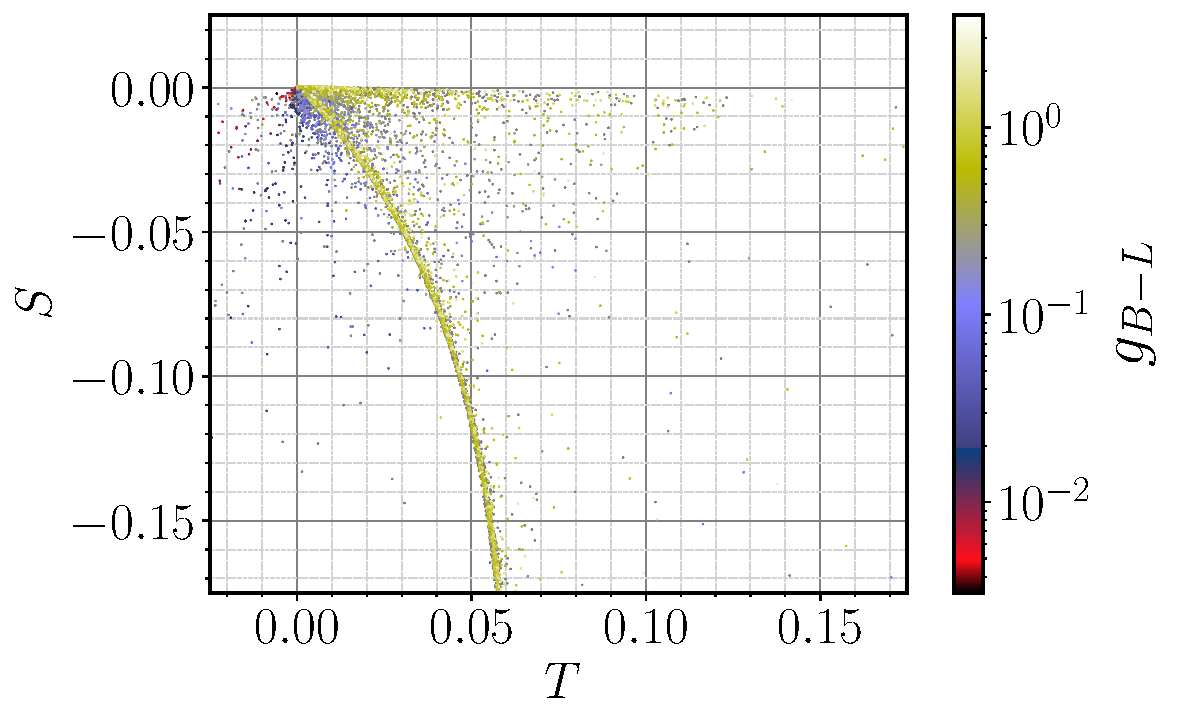
\includegraphics[width=0.32\textwidth]{Images/BLSM_2/TS_gBL.pdf}
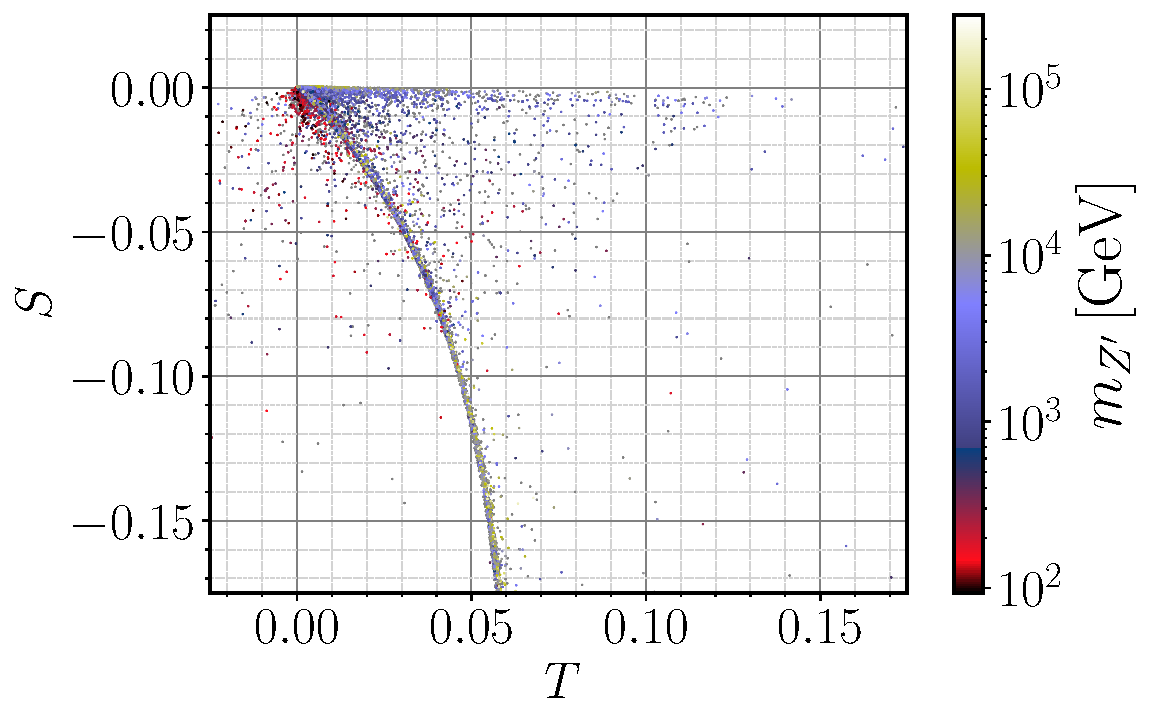
\includegraphics[width=0.32\textwidth]{Images/BLSM_2/TS_Zp.pdf}
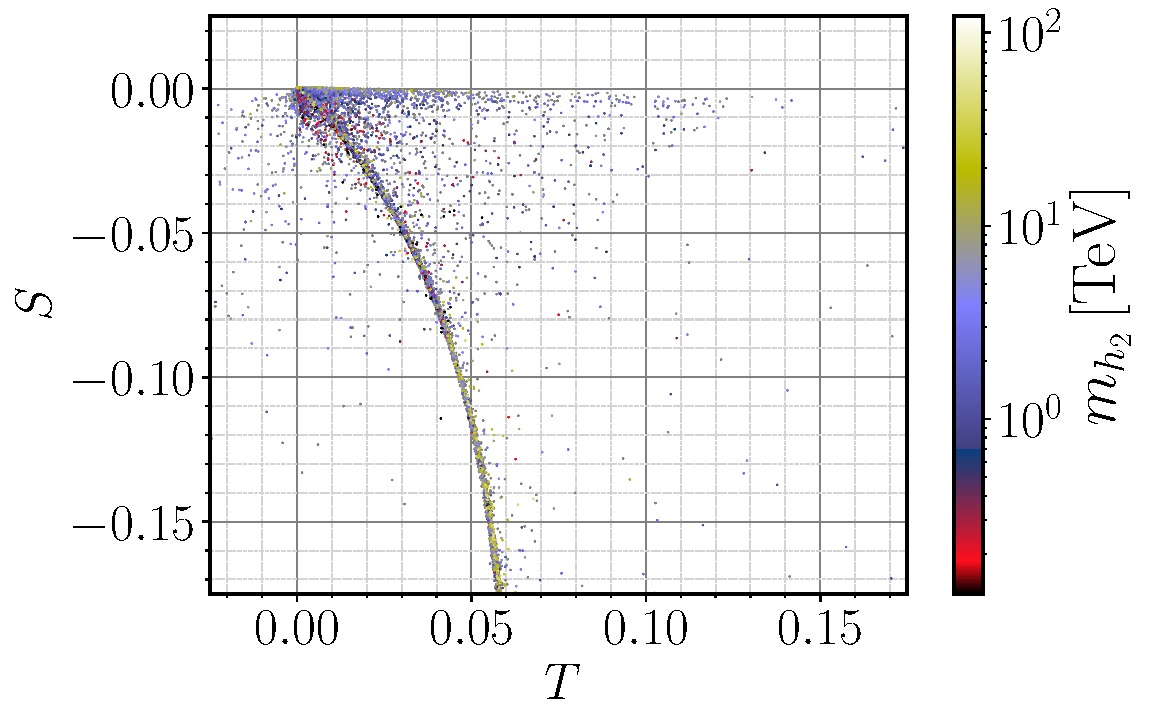
\includegraphics[width=0.32\textwidth]{Images/BLSM_2/TS_HP.pdf}
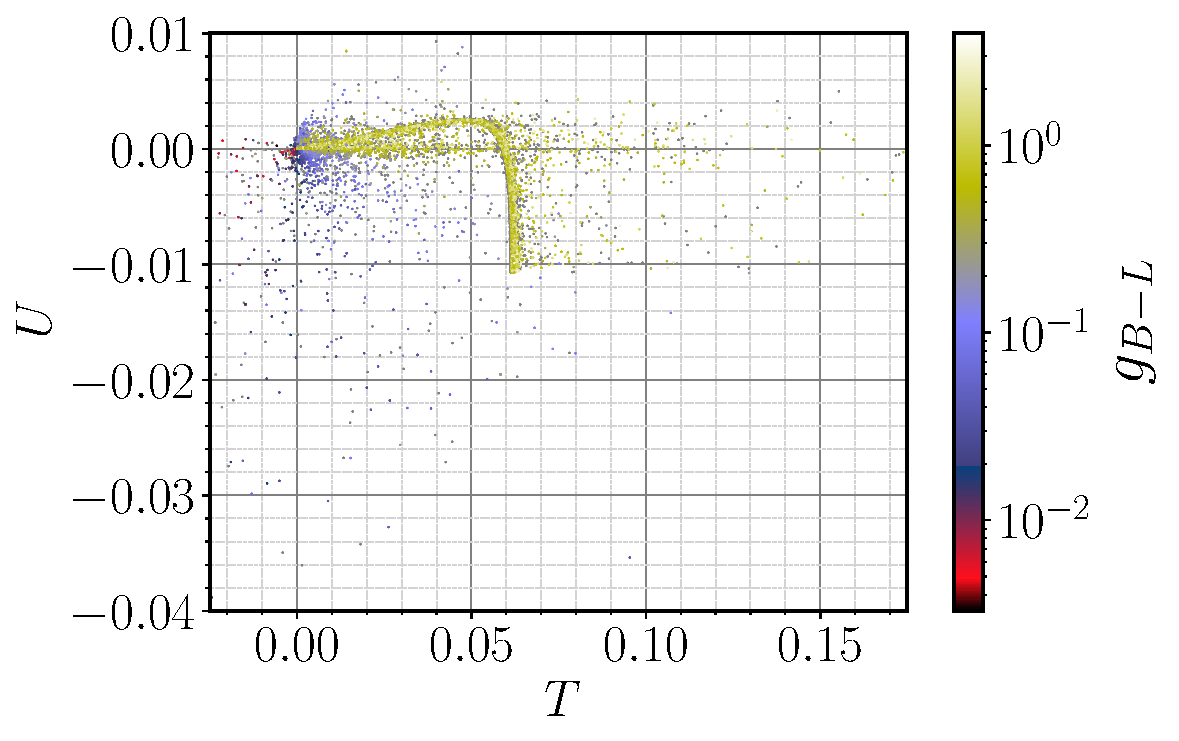
\includegraphics[width=0.32\textwidth]{Images/BLSM_2/TU_gBL.pdf}
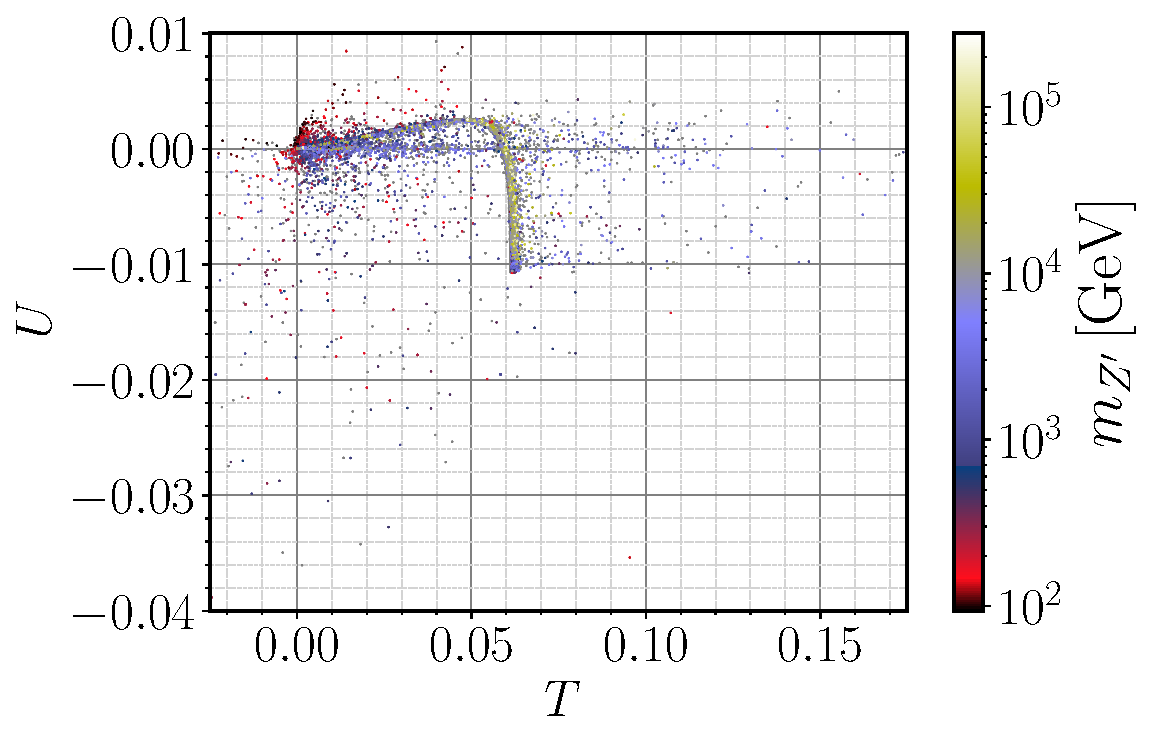
\includegraphics[width=0.32\textwidth]{Images/BLSM_2/TU_Zp.pdf}
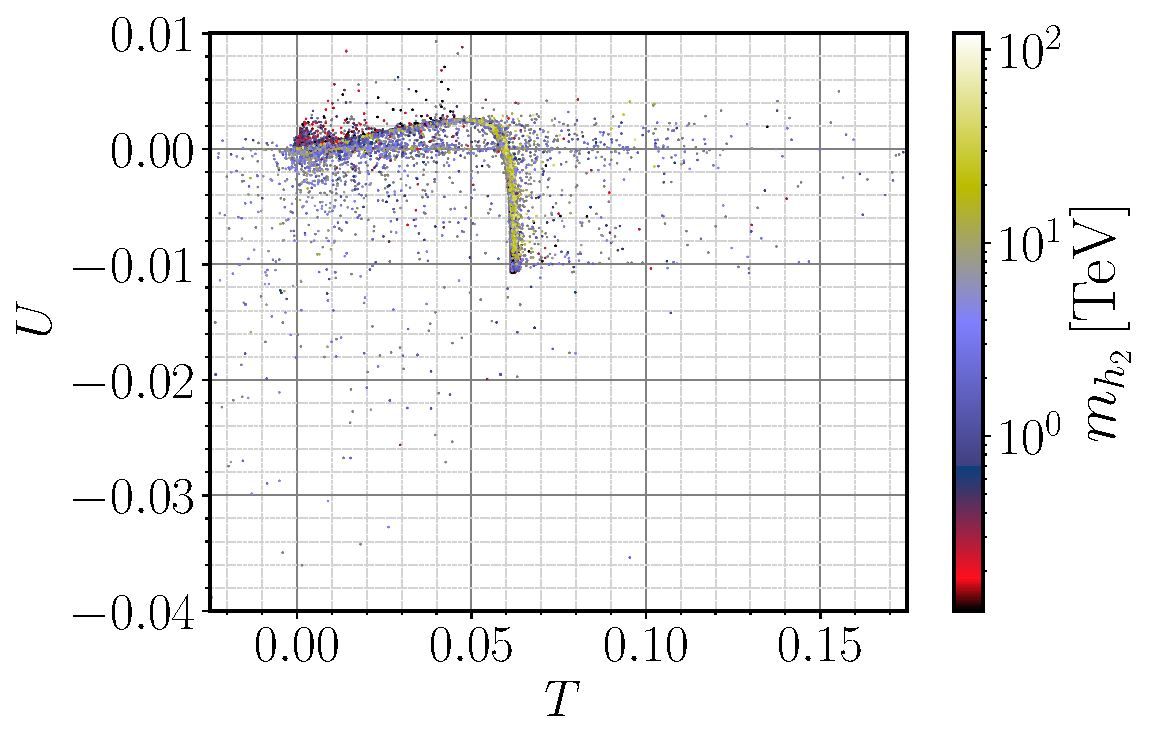
\includegraphics[width=0.32\textwidth]{Images/BLSM_2/TU_HP.pdf}
\caption{Scatter plots for the EW oblique corrections in the $ST$ (upper row) and $TU$ (lower row) planes. In the color scales, their correlations with the $\U{B-L}$ gauge coupling $g_{\ro{B-L}}$, $Z^\prime$ mass, $m_{Z^\prime}$, and second Higgs mass, $m_{h_2}$, are shown in left, 
middle and right panels, respectively. The points shown here are passed the unitarity constraints in \texttt{SPheno 4.0.3} \cite{Porod:2003um,Porod:2011nf} as well as the Higgs phenomenology constraints in \texttt{HiggsBounds 4.3.1} \cite{Bechtle:2013wla} and \texttt{HiggsSignals 1.4.0} \cite{Bechtle:2013xfa}.}
\label{fig:STU-gBL_Zp_HP}
\end{figure}	

 We show in Fig.~\ref{fig:STU-lambda-excl} our results in the $ST$ (upper row) and $TU$ (lower row) planes where coloured points are consistent with EW precision observables at $95\%$ C.L.~whereas grey ones lie outside the corresponding ellipsoid of the best fit point and, thus, are excluded in our analysis. The color scales show correlations with the scalar quartic couplings $\lambda_{1,2,3}$.
%%%%%%%%%%%%%%%%%%%%%%%%%%
\begin{figure}[!htb]
\centering
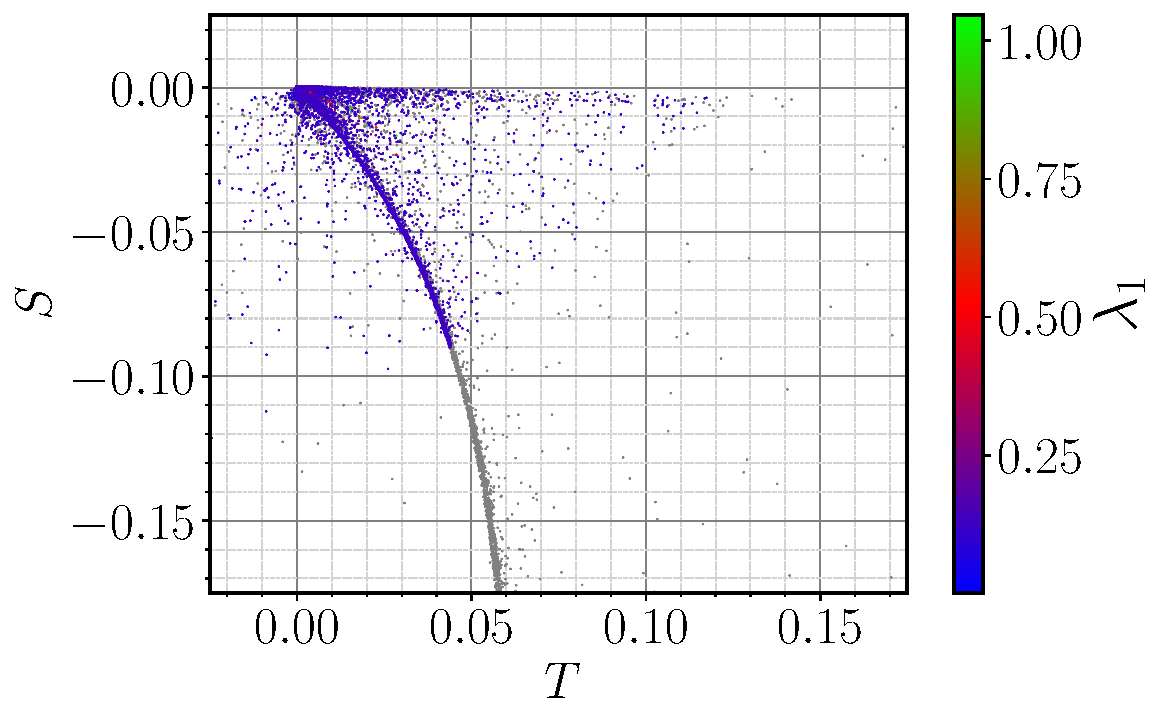
\includegraphics[width=0.32\textwidth]{Images/BLSM_2/TS_L1_EW.pdf}
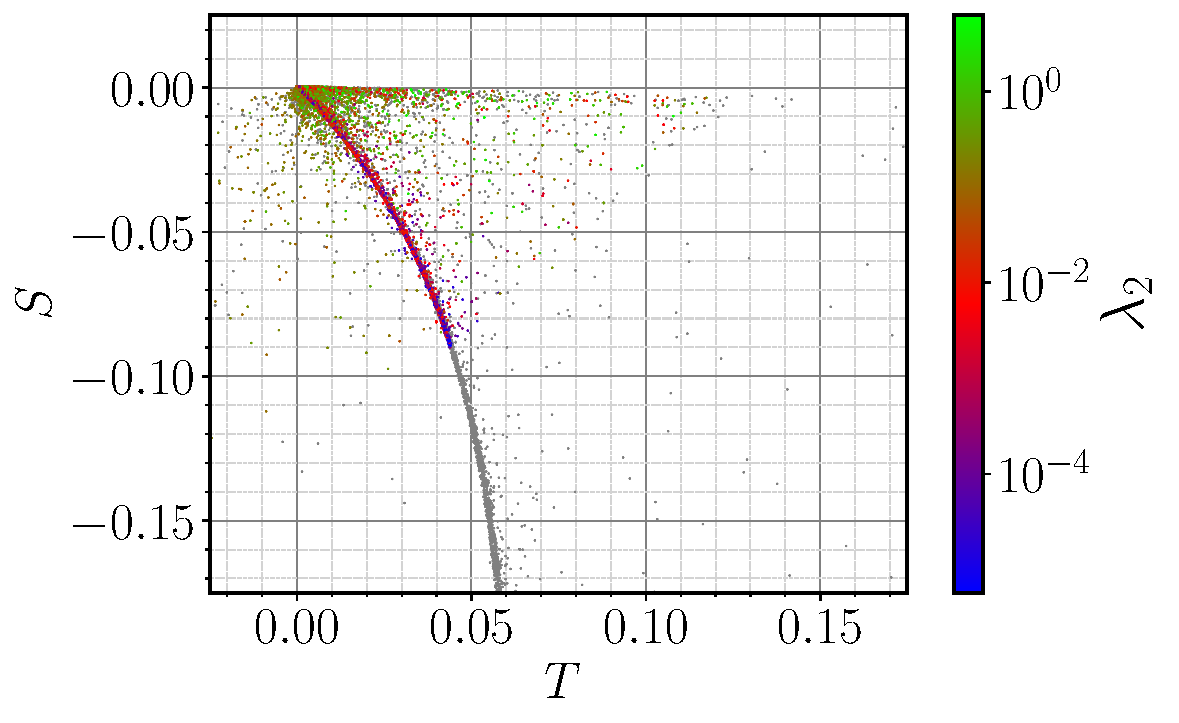
\includegraphics[width=0.32\textwidth]{Images/BLSM_2/TS_L2_EW.pdf}
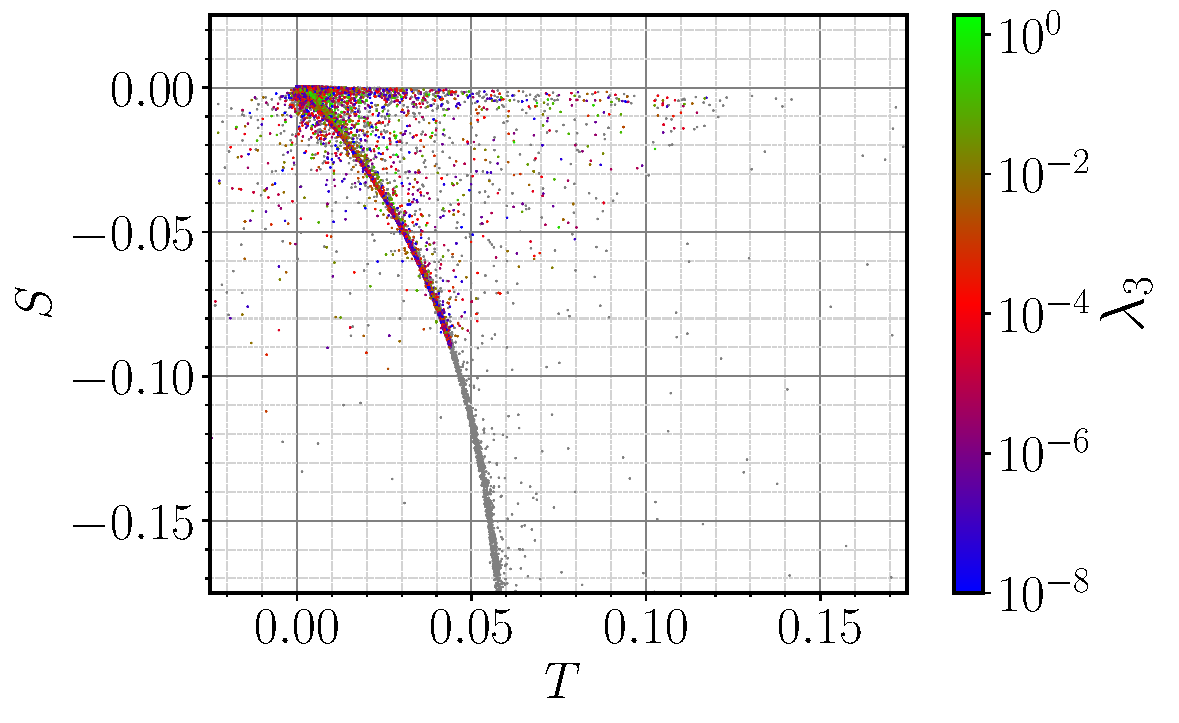
\includegraphics[width=0.32\textwidth]{Images/BLSM_2/TS_L3_EW.pdf}
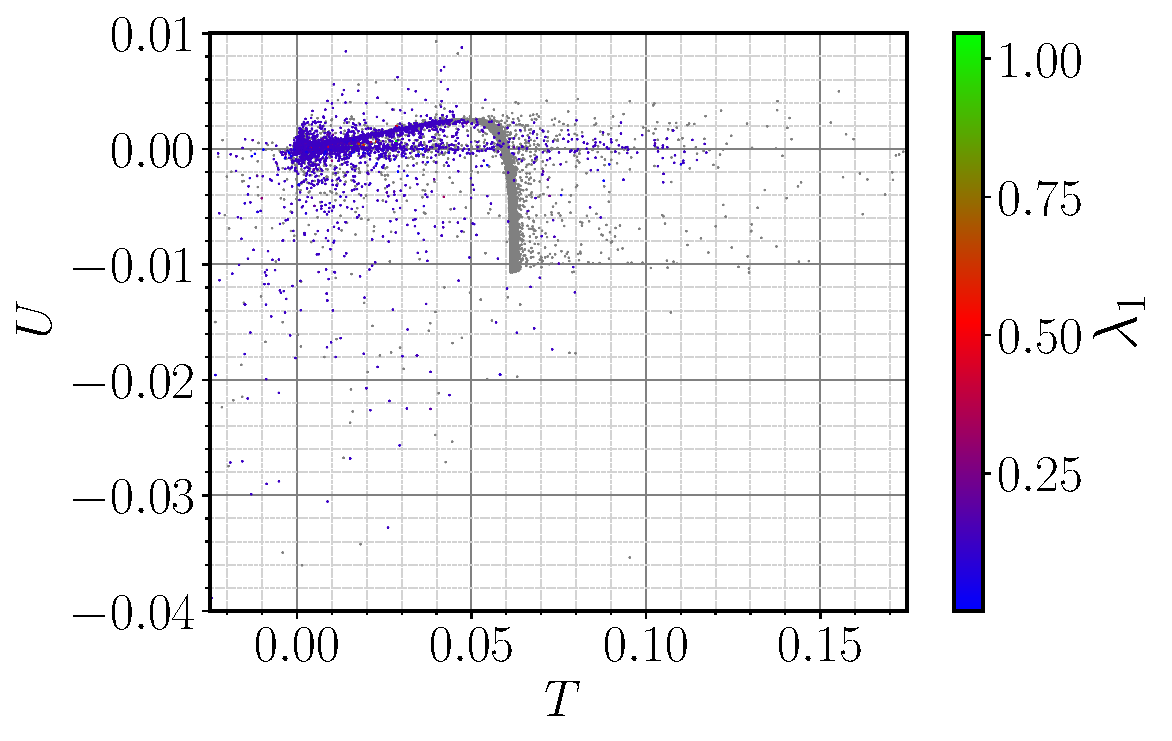
\includegraphics[width=0.32\textwidth]{Images/BLSM_2/TU_L1_EW.pdf}
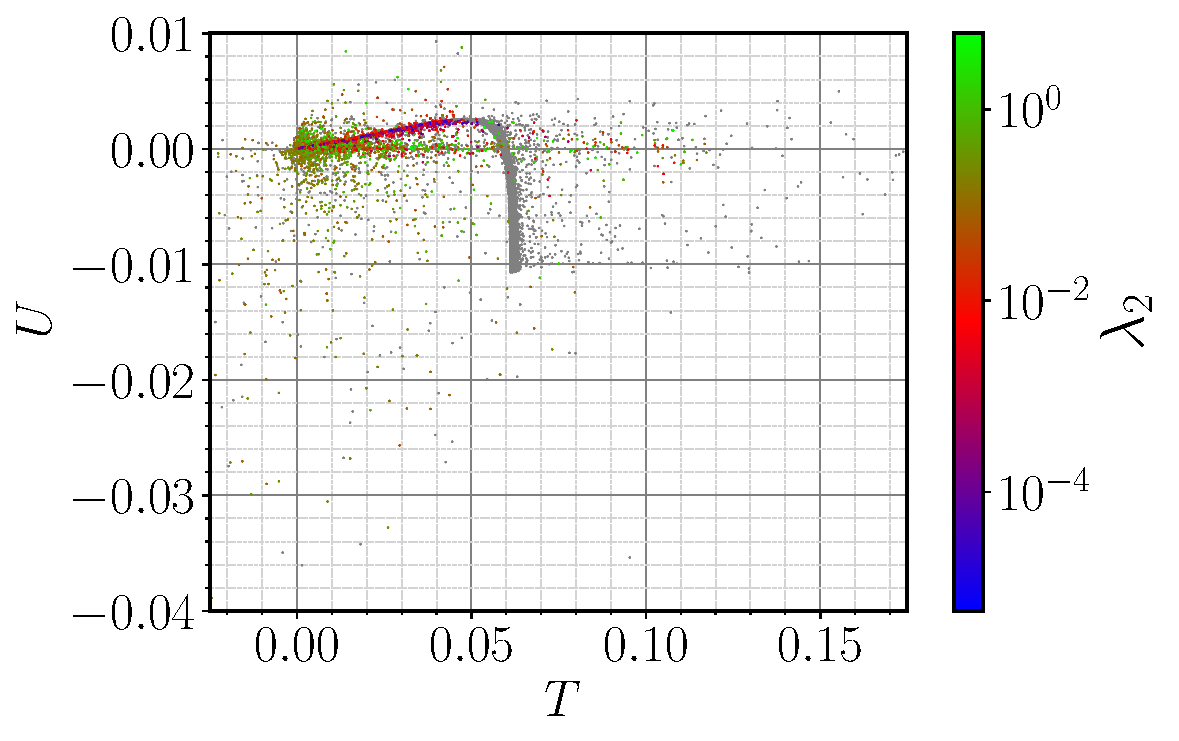
\includegraphics[width=0.32\textwidth]{Images/BLSM_2/TU_L2_EW.pdf}
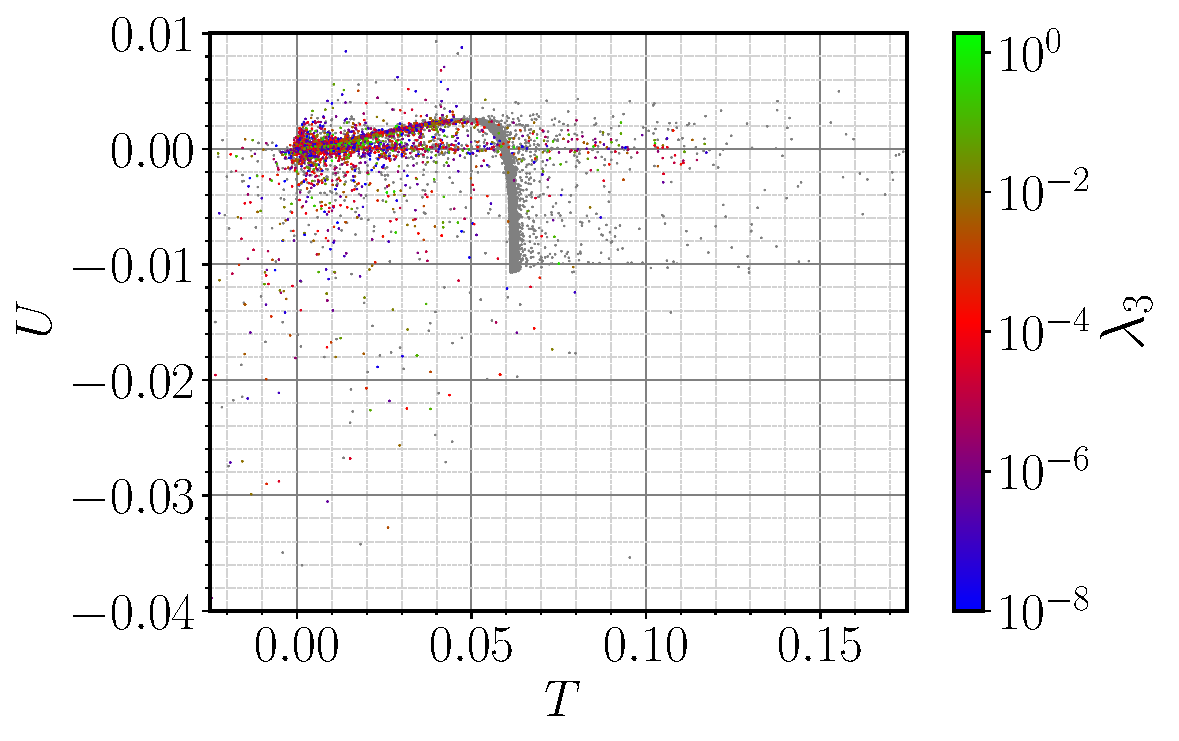
\includegraphics[width=0.32\textwidth]{Images/BLSM_2/TU_L3_EW.pdf}
\caption{Scatter plots for the EW oblique corrections in the $ST$ (upper row) and $TU$ (lower row) planes versus the scalar quartic couplings $\lambda_{1,2,3}$ shown in the color scale.
Accepted points lying within a $95\%$ C.L.~ellipsoid of the best fit point, and hence satisfying the EW precision constraints, are given in color whereas grey points are excluded. Other constraints are the same as in Fig.~\ref{fig:STU-gBL_Zp_HP}.  }
\label{fig:STU-lambda-excl}
\end{figure}	


\subsubsection{$Z^\prime$ Constraints and its effect on the Higgs singlet}

%\subsubsection{Higgs Constraints}

We then confront the surviving scenarios (coloured points in Figs.~\ref{fig:STU-lambda-excl} and \ref{fig:STU-gBL_Zp_HP}) with collider bounds on Higgs searches at the LHC, LEP and the Tevatron through \texttt{HiggsBounds 4.3.1} and \texttt{HiggsSignals 1.4.0}. 
%
Additionally we also ensured that a SM Higgs candidate is assured, $m_{h_1} = 125.10 \pm 0.14~\textrm{GeV}$. 

Now having verified the scalar sector we can access viability of the surviving points from the perspective of direct collider searches for a new $Z^\prime$ gauge boson. We can see the impact of all layered cuts in the following figures reflecting Higgs and Gauge physics cuts. We show in Fig.~\ref{fig:Plots1} the scenarios generated in our parameter space scan that have passed all theoretical and experimental.
%
%%%%%%%%%%%%%%%%%%%%%%%%%%
\begin{figure}[!htb]
	\centering
	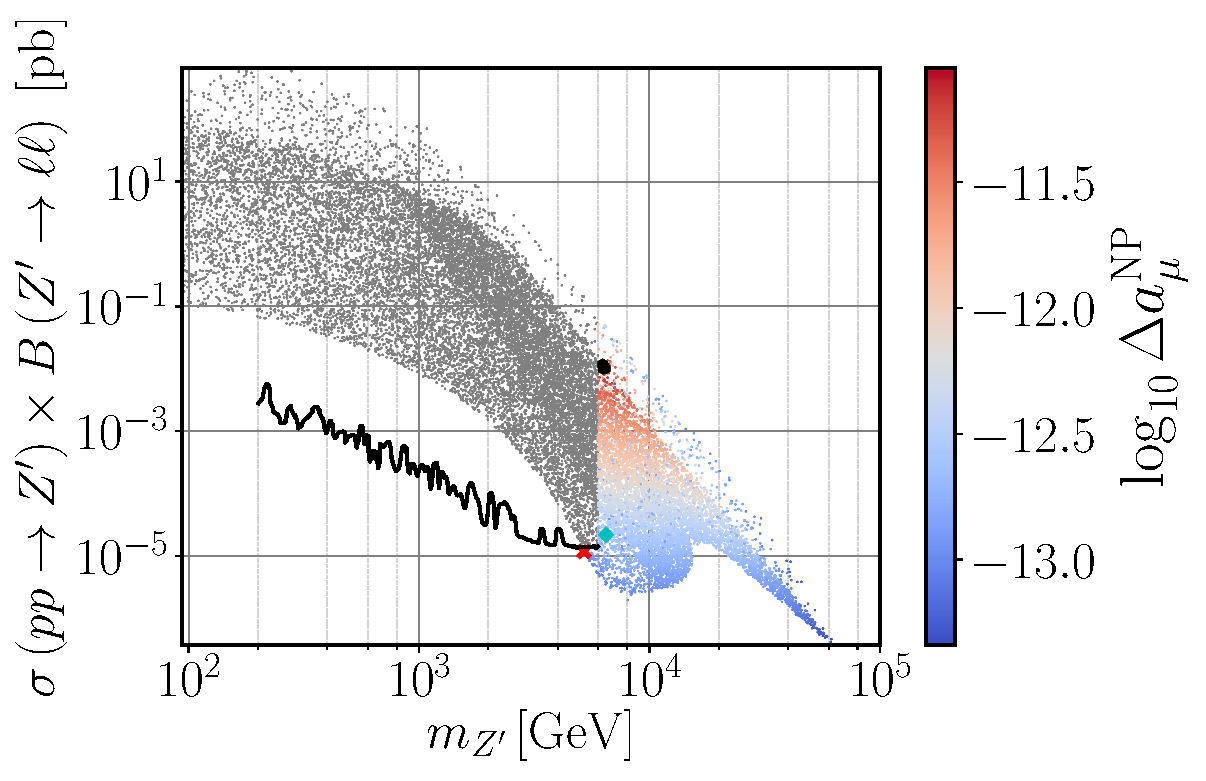
\includegraphics[scale=0.37]{Images/BLSM_2/mZp_Xsec_Amu.pdf}
	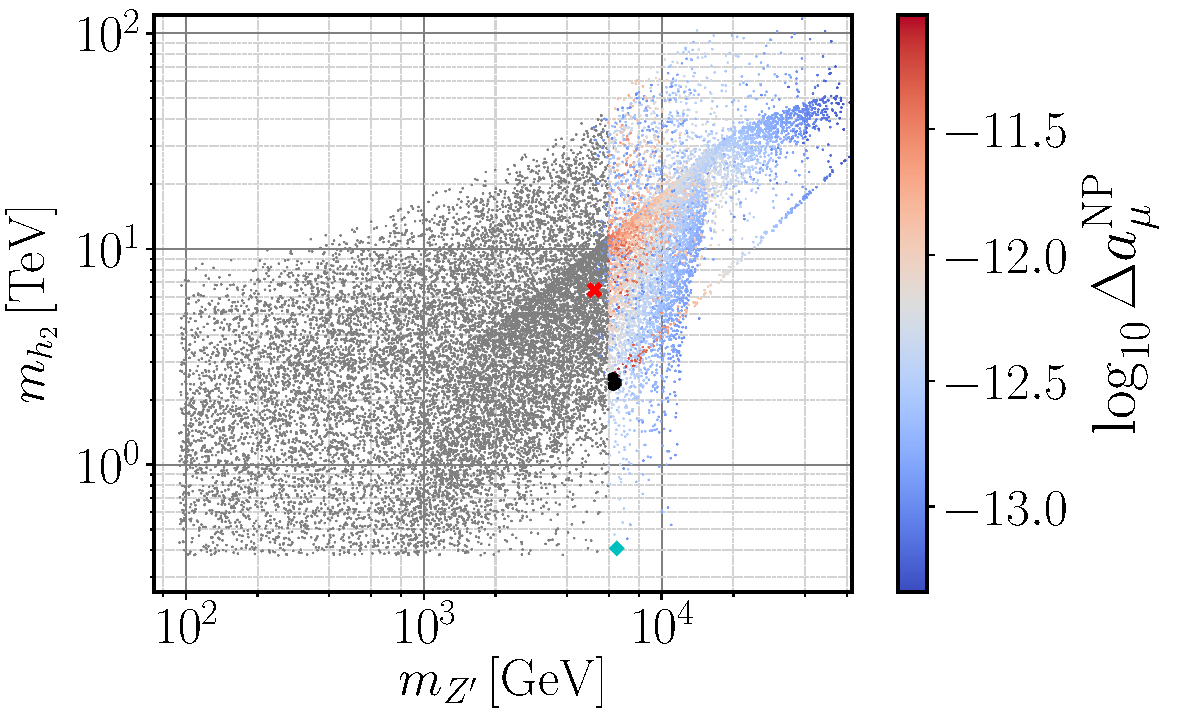
\includegraphics[scale=0.37]{Images/BLSM_2/mZp_Mhp_Amu.pdf}
	\caption{Scatter plots showing the $Z^\prime$ Drell-Yan production cross section times the decay branching ratio into a pair of electrons and muons (left panel) and the new scalar mass $m_{h_2}$ (right panel) as functions of $m_{Z^\prime}$ and the new physics (NP) contributions 
	to the muon $\Delta a_\mu$ anomaly. The solid line represents the current ATLAS expected limit on the production cross section times branching ratio into a pair of leptons at $95\%$ C.L.~ taken from Ref.~\cite{Aad:2019fac}.  Coloured points have survived all theoretical and experimental 
	constraints while grey points are excluded by direct $Z^\prime$ searches at the LHC. The six highlighted points in both panels denote the benchmark scenarios described in Tab.~\ref{tab:bench}. These are represented by the red cross for the lightest $Z^\prime$ scenario (first row), cyan diamond for the lightest $h_2$ scenario (second row) and the black dots (last four rows).}
	\label{fig:Plots1}
\end{figure}	
%%%%%%%%%%%%%%%%%%%%%%%%%%

Here, on the left panel of Fig.~\ref{fig:Plots1}, we show the $Z^\prime$ production cross section times its branching ratio to the first - and second-generation leptons, $\sigma B \equiv \sigma \left( pp \to Z^\prime \right) \times B \left( Z^\prime \to \ell \ell \right) $ with $\ell = e,\mu$, as a function of the new vector boson mass and the new physics contribution to the muon anomalous magnetic moment $\Delta a^{\textrm{NP}}_\mu$ (color scale). 
%
On the right panel, we show the new scalar mass, $m_{h_2}$, as a function of the $Z^\prime$ Mass. 
%
All points above the red dashed line are excluded at $95\%$ C.L.~by the upper expected limit on $Z^\prime$ direct searches at the LHC by the ATLAS experiment and are represented in gray shades. 
%
Darker shades denote would-be-scenarios with larger values of $\Delta a^{\ro{NP}}_\mu$ while the smaller contributions to this observable are represented with the lighter shades. The red cross in our figures signals the lightest $Z^\prime$ found in our scan which we regard as a possible early-discovery (or early-exclusion) benchmark point in the forthcoming LHC runs. Such a benchmark point is shown in the first line of Tab.~\ref{tab:bench}. On the right panel, we notice that the new scalar bosons can become as light as $400~\ro{GeV}$, with $Z^\prime$ masses being above $5.2~\ro{TeV}$. Such a moderately large minimal value for the new Higgs boson mass results from the fact that both the $h_2$ and the $Z'$ bosons share a common VEV in their mass forms as seen in Eqs.~\eqref{eq:simplify} and \eqref{eq:mZ}. Then, while direct searches at the LHC for a B-L-SM $Z'$ boson keep pushing its mass to larger values, the new Higgs boson mass also increases linearly with $m_{Z'}$ according to
\begin{equation}
	m_{h_2} \approx \sqrt{\frac{\lambda_2}{2}} \frac{m_{Z'}}{g_{\mathrm{B-L}}}\,.
\end{equation} 
Furthermore, neither $\lambda_2$ can be arbitrarily small (see Fig.~\ref{fig:STU-lambda-excl} central panels), not $g_{\mathrm{B-L}}$ can be arbitrarily large (see Fig.~\ref{fig:STU-gBL_Zp_HP} left panels) in order to compensate an increase in $m_{Z'}$. We highlight with a cyan diamond the benchmark point with the lightest $h_2$ boson within this range. This point is shown in the second line of Tab.~\ref{tab:bench}.
\setlength{\tabcolsep}{2pt} % Default value: 6pt
\renewcommand{\arraystretch}{1} % Default value: 1
%
\begin{table}[htb!]
\begin{center}
		\begin{tabular}{cccccccccc}
			$m_{Z^\prime}$ & $m_{h_2}$ &  $x$& $ \log_{10} \Delta a_\mu^{\ro{NP}}$ & $\sigma B$ & $\theta_W^\prime$ & $\log_{10}\alpha_h$ & $\g{B-L}{}$ & $\g{YB}{}$ & 
			$ \g{L}{\ell \ell Z^\prime} = \g{R}{\ell \ell Z^\prime}$ % & $\delta$ 
			\vspace{1mm}
			\\
			\hline \vspace{-1mm} \\ 
			%%%%%%%%%%
$5.199$    & $6.41$     & $15.4$    & $-13.01$       & $1.16 \times 10^{-5}$   & $\approx 0$                    & $-5.18$     & $0.17$   & $2.0\times 10^{-5}$    & $0.08$  %  &   $2.35\sigma$  
\vspace{1mm}  \\ 
$6.478$    & $0.41$     & $9.77$    & $-12.57$       & $2.15 \times 10^{-5}$   & $3.22\times 10^{-7}$      & $-5.85$     & $0.34$   & $1.7\times 10^{-3}$    & $0.17$  %  &   $2.35\sigma$ 
\vspace{1mm}   \\ 
$6.371$    & $2.34$     & $1.08$   & $-11.05$        & $0.01$                           & $1.05\times 10^{-6}$      & $-7.31$     & $1.97$   & $2.1\times 10^{-3}$    & $0.98$   %  &  $2.34\sigma$ 
\vspace{1mm}    \\ 
$6.260$    & $2.31$     & $1.15$   & $-11.07$        & $0.01$                           & $5.87\times 10^{-5}$      & $-2.79$     & $1.87$   & $0.125$                        & $0.94$  %  &  $2.34\sigma$  
\vspace{1mm}   \\ 
$6.477$    & $2.40$      & $1.14$   & $-11.08$       & $0.01$                           & $2.75\times 10^{-5}$      & $-4.29$     & $1.93$   & $0.06$                          & $0.97$  %  &  $2.34\sigma$ 
\vspace{1mm}    \\ 
$6.252$    & $2.53$     & $1.28$   & $-11.08$        & $0.01$                           & $\approx 0$                    & $-8.65$     & $1.86$   & $1.6\times 10^{-5}$     & $0.93$   %  &  $2.34\sigma$ 
\vspace{1mm}   \\ 
\end{tabular}
		\caption{A selection of five benchmark points represented in Figs.~\ref{fig:Plots1} and \ref{fig:Plots4} to \ref{fig:Plots2}. The $m_{Z^\prime}$, $m_{h_2}$ and $x$ parameters are given in TeV. The second line represents a point with lightest possible $h_2$ while the first one shows the lightest allowed $Z^\prime$ boson found in our scan. The last four lines show four points that yield 
a minimal tension $3.28$ standard deviations, with the combined theoretical and experimental error of the muon $(g-2)_\mu$ anomaly.}
		\label{tab:bench}
\end{center}
\end{table}
\setlength{\tabcolsep}{6pt} % Default value: 6pt
\renewcommand{\arraystretch}{1} % Default value: 1
%

\subsubsection{Implications of direct $Z^\prime$ searches at the LHC for the $\left(g-2\right)_\mu$ anomaly}

Looking again to Fig.~\ref{fig:Plots1} (left panel), we see that there is a dark-red region where $\Delta a_\mu^{\ro{NP}}$ can be enhanced up to a maximum of $\Delta a_\mu^{\mathrm{NP}} = 8.9 \times 10^{-12}$ for a range of $m_{Z^\prime}$ boson masses approximately between $6.3~\ro{TeV}$ and $6.5~\ro{TeV}$, representing a very small improvement in comparison to the SM prediction. Such a mass region is particularly interesting as it can be probed by the forthcoming LHC runs. If a $Z^\prime$ boson discovery remains elusive, it can exclude a possibility of alleviating the tension between the measured and the SM prediction for the muon $\left(g-2\right)_\mu$ anomaly in the context of the B-L-SM. However, note that with new measurements at the E989 experiment at Fermilab, if a partial reduction in the current discrepancy is observed, the B-L-SM prediction may become an important result and a motivation for future $Z'$ searches at the LHC. Note, such maximal $\Delta a^{\ro{NP}}_\mu$ values represent a rather small region of scattered red points where the new scalar boson mass takes values of a few TeV. Furthermore, in some scenarios represented by the second and third lines in Tab.~\ref{tab:bench}, the $\theta_W^\prime$ and $\alpha_h$ angles are not vanishingly small which may hint certain possibilities for observing both a new scalar and new vector boson in this region.
%%%%%%%%%%%%%%%%%%%%%%%%%
\begin{figure}[!htb]
	\centering
	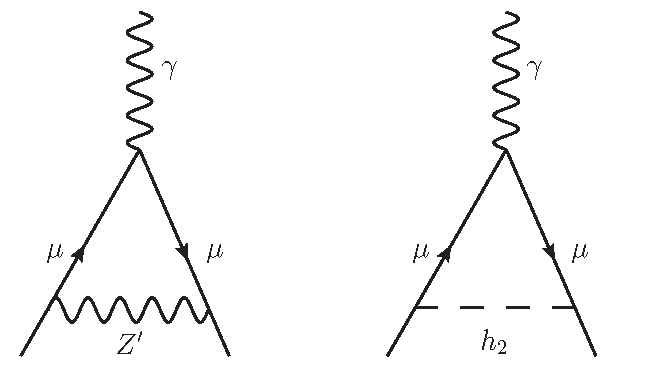
\includegraphics[scale=0.75]{Images/BLSM_2/g-2.pdf}
	\caption{One-loop diagrams contributing to $\Delta a_\mu^{\ro{NP}}$ in the B-L-SM.}
	\label{fig:g-2}
\end{figure}	
%%%%%%%%%%%%%%%%%%%%%%%%%

New physics contributions $\Delta a_\mu^{\ro{NP}}$ to the muon anomalous magnetic moment are given at one-loop order by the Feynman diagrams depicted in Fig.~\ref{fig:g-2}.
%
Since the couplings of a new scalar $h_2$ to the SM fermions are suppressed by a factor of $\sin \alpha_h$, which we find to be always smaller than $0.002$ as can be seen in the bottom panel of Fig.~\ref{fig:Plots4}, the right diagram in Fig.~\ref{fig:g-2}, which scales as $\Delta a_\mu^{h_2} \propto \tfrac{m_\mu^2}{m_{h_2}^2}\left(y_\mu \sin \alpha_h\right)^2$ with $y_\mu = Y_e^{22}$, provides sub-leading contributions to $\Delta a_\mu$.
%
Furthermore, as we show in the top-left panel of Fig.~\ref{fig:Plots4} the new scalar boson mass, which we have found to satisfy $m_{h_2} \gtrsim 400~\ro{GeV}$, is not light enough to compensate the smallness of the scalar mixing angle. Conversely, and recalling that all fermions in the B-L-SM transform non-trivially under $\U{B-L}$, the new $Z^\prime$ boson can have sizeable couplings to fermions via gauge interactions proportional to $\g{B-L}{}$ and $\g{YB}{}$, essentially constrained by four fermion contact interactions. 


Therefore, the left diagram in Fig.~\ref{fig:g-2} provides the leading contribution to the $\left(g-2\right)_\mu$ in the model under consideration.
%%%%%%%%%%%%%%%%%%%%%%%%%%
\begin{figure}[!htb]
	\centering
	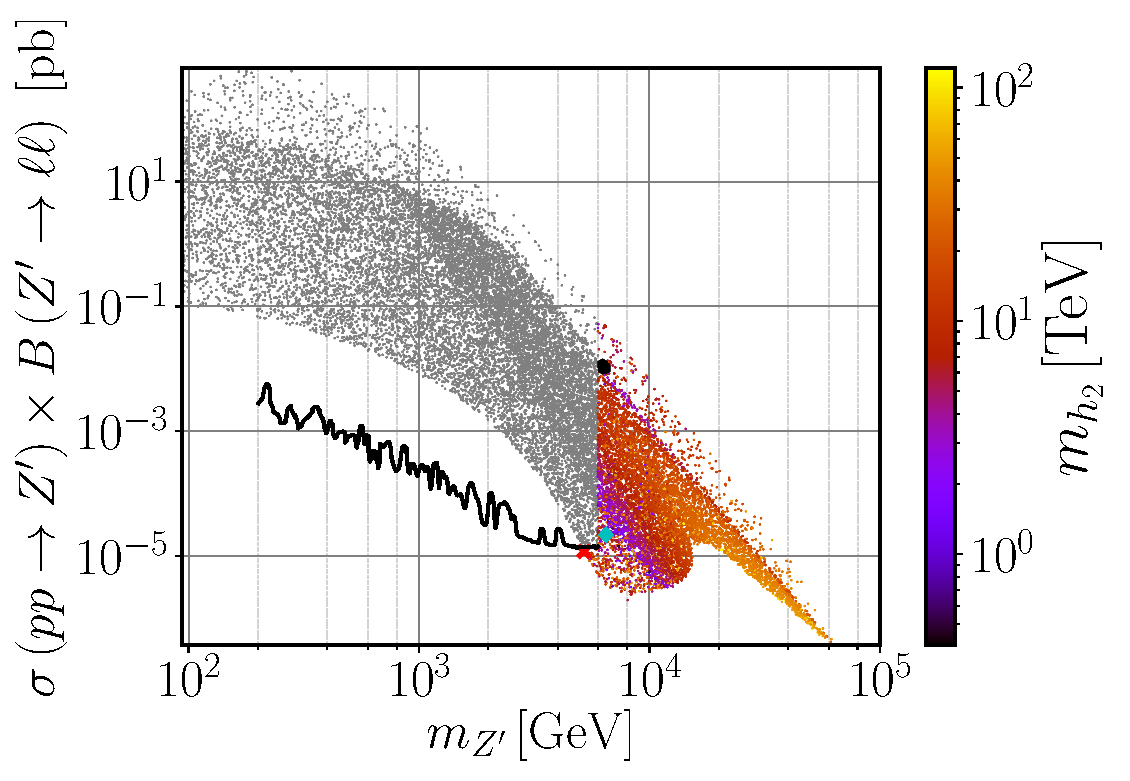
\includegraphics[scale=0.37]{Images/BLSM_2/mZp_Xsec_mh2.pdf}
	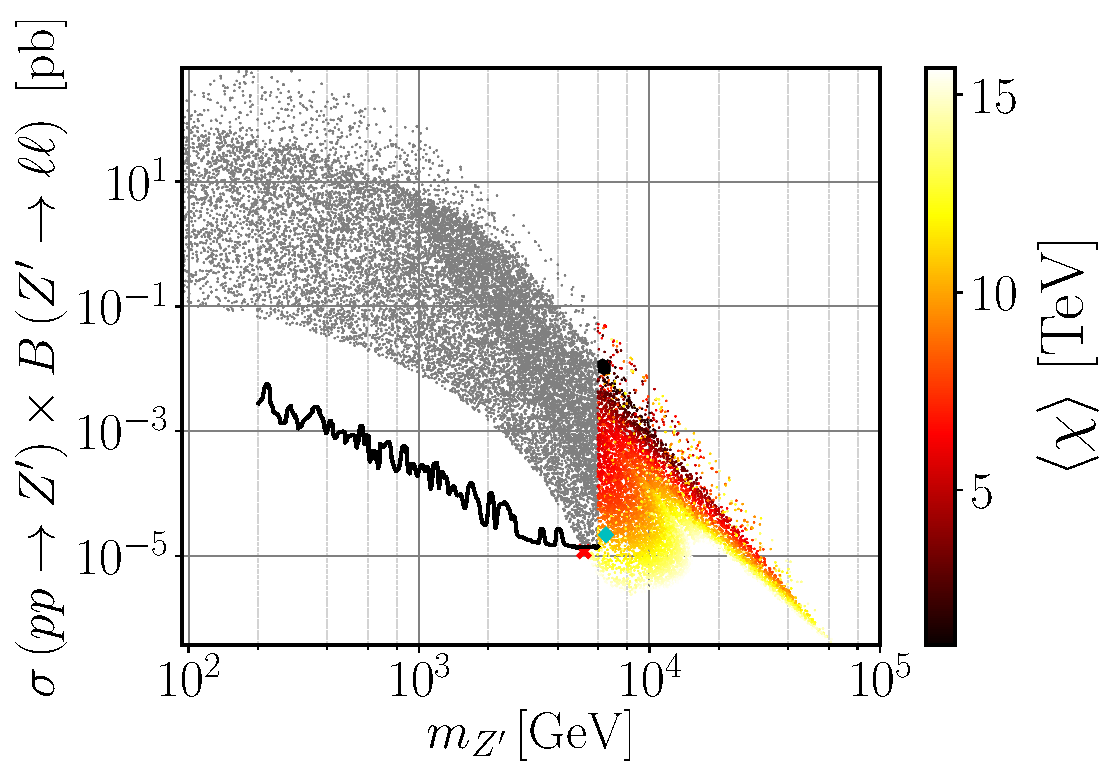
\includegraphics[scale=0.37]{Images/BLSM_2/mZp_Xsec_VEV.pdf}
	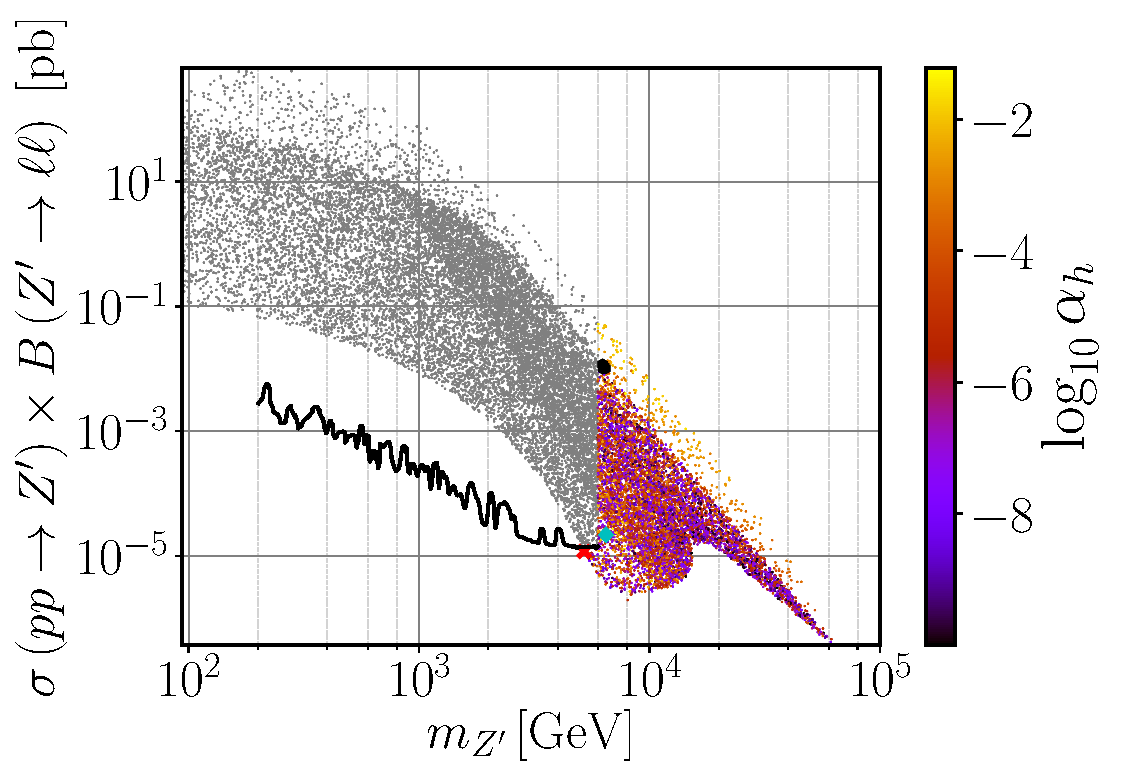
\includegraphics[scale=0.37]{Images/BLSM_2/mZp_Xsec_alpha.pdf}	
	\caption{Scatter plots showing the $Z^\prime$ Drell-Yan production cross section times the decay branching ratio into a pair of electrons and muons in terms of the $m_{Z^\prime}$ boson mass. The colour gradation represents the new scalar mass (top-left), the $\U{B-L}$-breaking VEV (top-right) and the scalar mixing angle (bottom). The notation is the same as in Fig.~\ref{fig:Plots1} (left). }
	\label{fig:Plots4}
\end{figure}	
%%%%%%%%%%%%%%%%%%%%%%%%%%
In particular, $\Delta a_\mu^{Z^\prime}$ can be written as
\begin{equation}
\Delta a_\mu^{Z^\prime} = \tfrac{1}{4 \pi^2} \tfrac{m_\mu^2}{m_{Z^\prime}^2} \left[\g{L}{\mu \mu Z^\prime} \g{R}{\mu \mu Z^\prime} g_{\ro{FFV}}\left(\frac{m_\mu^2}{m_{Z'}^2}\right) + \left({\g{L}{\mu \mu Z^\prime}}^2 + {\g{R}{\mu \mu Z^\prime}}^2\right) f_{\ro{FFV}}\left(\frac{m_\mu^2}{m_{Z'}^2}\right) \right]
\label{eq:ZpContribution}
\end{equation}
where the left- and right-chiral projections of the charged lepton couplings to the $Z^\prime$ boson, $\g{L}{\ell \ell Z^\prime}$ and $\g{R}{\ell \ell Z^\prime}$, respectively, can be approximated as follows
\begin{equation}
\begin{aligned}
    \g{L}{\ell \ell Z^\prime} &\simeq \frac12\g{B-L}{} 
    +\frac14 \g{YB}{}
    + \frac{1}{32} \left(\frac{v}{x}\right)^2 \frac{\g{YB}{}}{\g{B-L}{2}} \left(\g{Y}{2} - g^2 \right)\,,
    \\
    \g{R}{\ell \ell Z^\prime} &\simeq \frac12\g{B-L}{}
    + \frac12\g{YB}{} 
    + \frac{1}{16} \left(\frac{v}{x}\right)^2 \frac{\g{YB}{}}{\g{B-L}{2}}\g{Y}{2}\,,
\end{aligned}\label{eq:gllZ}
\end{equation}
%

to the second order in $v/x$-expansion. The regions of the parameter space that we are exploring feature a heavy $Z'$ boson such that $m_\mu^2 \ll m_{Z'}^2$. 
In such a limit the loop functions $g_{\ro{FFV}}\left(\tfrac{m_\mu^2}{m_{Z'}^2}\right)$ and $f_{\ro{FFV}}\left(\tfrac{m_\mu^2}{m_{Z'}^2}\right)$tend to the values $g_{\ro{FFV}}\left(0\right) \to 4$ and $f_{\ro{FFV}}\left(0\right) \to -\tfrac{4}{3}$ where Eq.~\eqref{eq:ZpContribution} can be approximated to
\begin{equation}
\Delta a_\mu^{Z^\prime} \approx \tfrac{1}{3 \pi^2} \tfrac{m_\mu^2}{m_{Z^\prime}^2} \left[3 \g{L}{\mu \mu Z^\prime} \g{R}{\mu \mu Z^\prime} - \left({\g{L}{\mu \mu Z^\prime}}^2 + {\g{R}{\mu \mu Z^\prime}}^2\right) \right]\,.
\label{eq:ZpContribution-2}
\end{equation}
If $v/x \ll 1$, corresponding to the lighter shades of the color scale in the top-right panel of Fig.~\ref{fig:Plots4}, we can further approximate\footnote{ Even the yellow region in Fig.~\ref{fig:Plots4} has $v<x$ thus, expanding around small $v/x$ also provides a reliable approximation.}
\begin{equation}
\g{L}{\ell \ell Z^\prime} \simeq \frac12\left(\g{B-L}{} + \dfrac{1}{2} \g{YB}{} \right)\,,
\qquad
\g{R}{\ell \ell Z^\prime} \simeq \frac12\left(\g{B-L}{} + \g{YB}{}\right)\,. 
\label{eq:gLgR-simp}
\end{equation}
With this, the $Z'$ contribution to the muon anomalous magnetic moment can be recast as
\begin{equation}
\Delta a_\mu^{Z^\prime} \simeq \dfrac{1}{48 \pi^2} \dfrac{m_\mu^2}{m_{Z^\prime}^2} \left[6 g_{\ro{B-L}}^{} g_{_{\ro{YB}}}^{} + 4 g_{\ro{B-L}}^{2} + g_{_{\ro{YB}}}^{2} \right] \,,
\label{eq:amu-simple}
\end{equation}
and for $\g{YB}{} \ll \g{B-L}{}$, which represents the majority of the points in our scan,
\begin{equation}
\Delta a_\mu^{Z^\prime} \simeq \dfrac{1}{12 \pi^2} \dfrac{m_\mu^2}{m_{Z^\prime}^2} \g{B-L}{2}\,.
\label{eq:amu-simple2}
\end{equation}
Note that, limits from four fermion contact interactions do not allow $\g{B-L}{}$ to be sufficiently large to contribute to a sizeable $\Delta a_\mu^{\rm NP}$ via  Eqs.~\eqref{eq:amu-simple} or \eqref{eq:amu-simple2}. In particular, we found that $\g{B-L}{}$ is always smaller than $1.97$ as depicted in the bottom panel of Fig.~\ref{fig:Plots3}. On another hand, limits on the $\theta_W^\prime$ mixing angle and from four-fermion contact interactions do not forbid an order one $\g{YB}{}$ coupling in the sparser upper edge of the top-left panel of Fig.~\ref{fig:Plots3}. It is indeed such a sizeable $\g{YB}{}$ that only slightly enhances the muon $(g-2)_\mu$ anomaly as can be seen in the red region of both plots in Fig.~\ref{fig:Plots1}. We have found four benchmark points represented by the black dots in Figs.~\ref{fig:Plots1} and \ref{fig:Plots4} to \ref{fig:Plots2}, where the tension between the current combined $1 \sigma$ error of the muon anomalous magnetic moment and the B-L-SM prediction is alleviated only by at most $0.01$ standard deviations in comparison to the SM, a totally negligible effect. These points are shown in the third to the sixth lines of Tab.~\ref{tab:bench}.
%%%%%%%%%%%%%%%%%%%%%%%%%%
\begin{figure}[!htb]
	\centering
	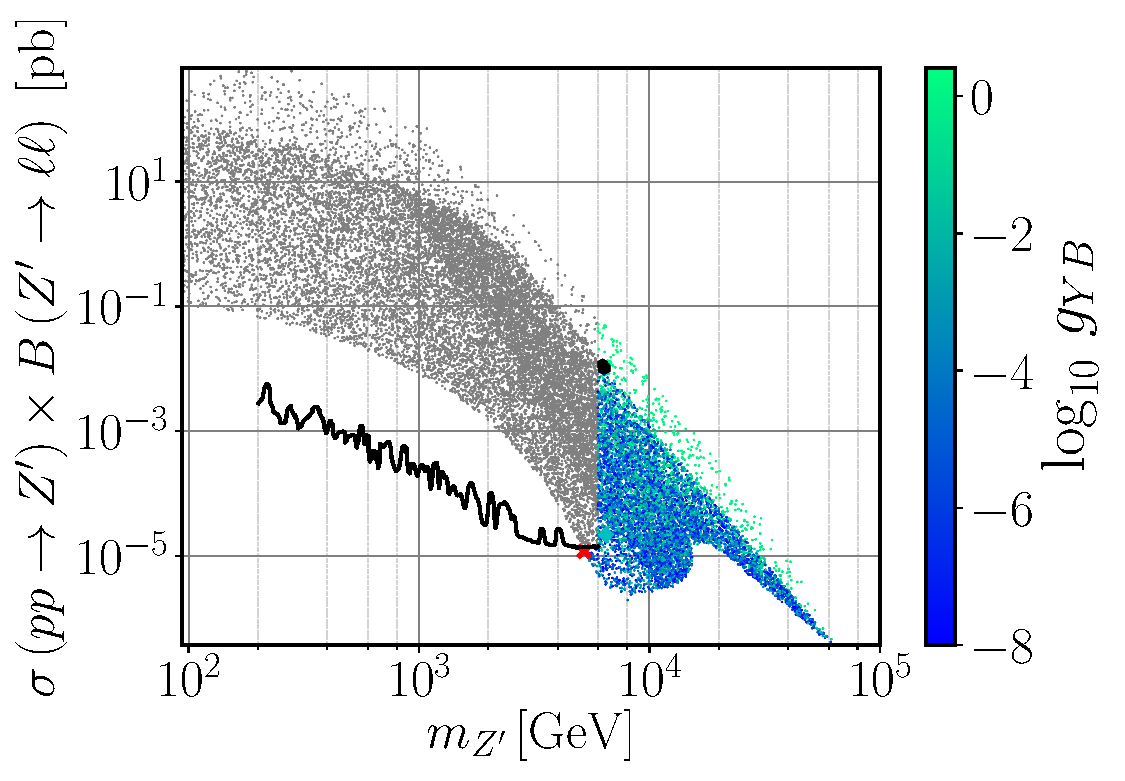
\includegraphics[scale=0.37]{Images/BLSM_2/mZp_Xsec_gYB.pdf}
	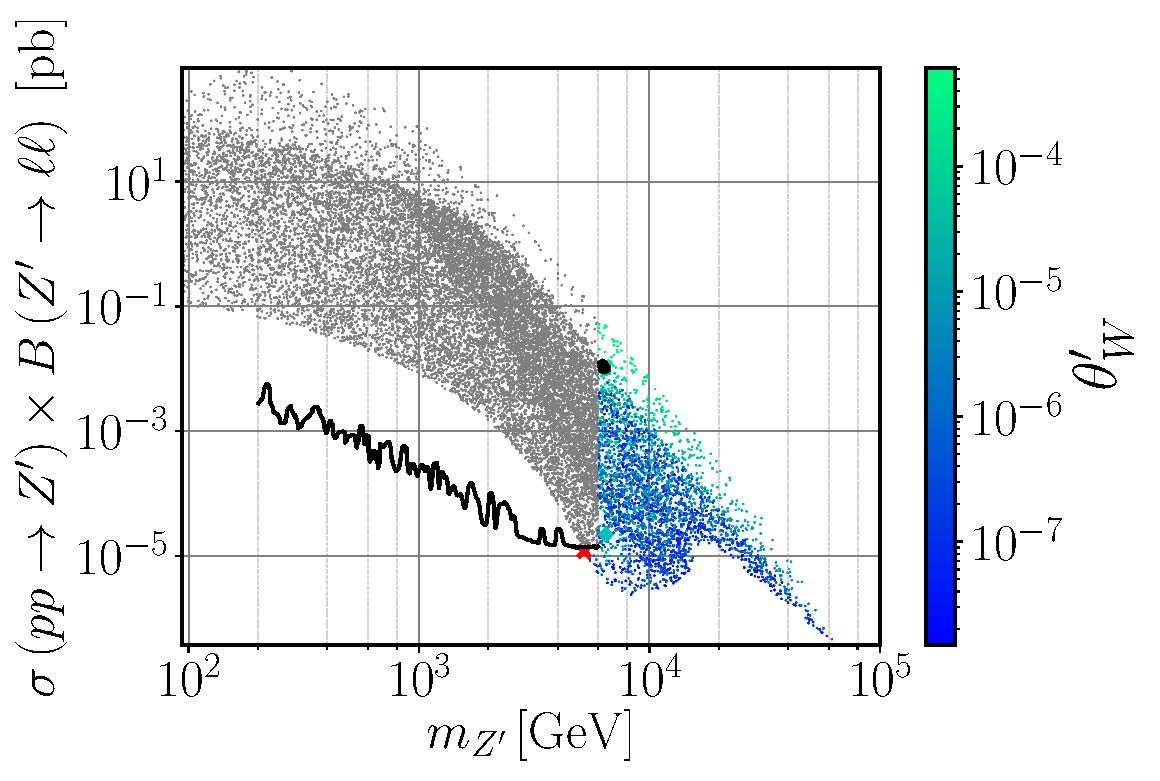
\includegraphics[scale=0.37]{Images/BLSM_2/mZp_Xsec_twp.pdf}
	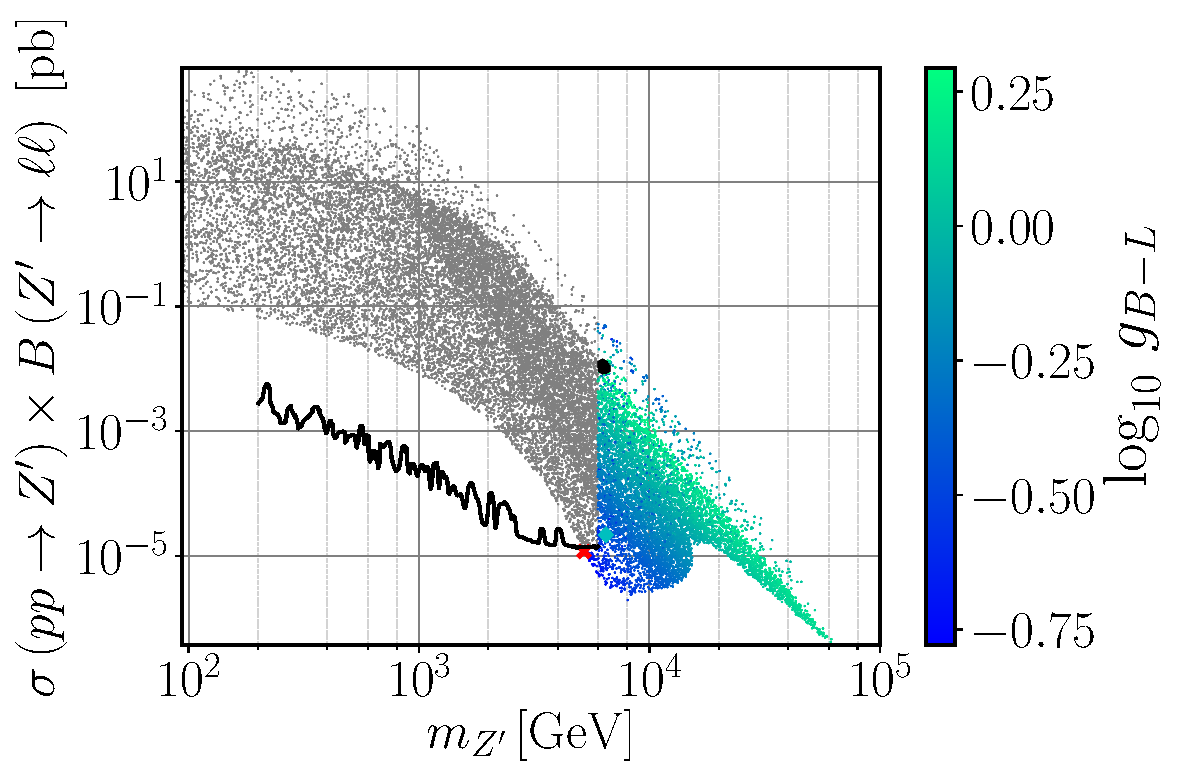
\includegraphics[scale=0.37]{Images/BLSM_2/mZp_Xsec_gBL.pdf}	
	\caption{The same as in Fig.~\ref{fig:Plots4} but with the colour scale representing the gauge-mixing parameters $\mathrm{g}_{\mathrm{YB}}$ (top-left) and $\theta_W^\prime$ (top-right), and the $\U{B-L}$ gauge coupling, $\mathrm{g}_{\mathrm{B-L}}$ (bottom).}
	\label{fig:Plots3}
\end{figure}	
%%%%%%%%%%%%%%%%%%%%%%%%%%

A close inspection of Fig.~\ref{fig:Plots1} (left panel) and Fig.~\ref{fig:Plots4} (top-right panel) reveals an almost one-to-one correspondence between the colour shades. This suggests that $\Delta a_\mu^{Z^\prime}$ must somehow be related to the \vev~$x$. To understand this behaviour, let us also look to Fig.~\ref{fig:Plots3} (top-left panel) where we see that the coupling $\g{YB}{}$ is typically very small apart from the green band on the upper edge where it becomes of order one. For the relevant parameter space regions, Eq.~\eqref{eq:mZ} is indeed a good approximation as was argued above. It is then possible to eliminate $\g{B-L}{}$ from Eq.~\eqref{eq:amu-simple2} and rewrite it as
\begin{equation}
    \Delta a_\mu^{Z^\prime} \simeq \dfrac{y_\mu^2}{96 \pi^2} \left(\dfrac{v}{x}\right)^2 \qquad \text{for} \qquad \g{YB}{} \ll \g{B-L}{} \,,
    \label{eq:amu-vev}
\end{equation}
which explains the observed correlation between both Fig.~\ref{fig:Plots1} (left panel) and Fig.~\ref{fig:Plots4} (top-right panel).
Note that this simple and illuminating relation becomes valid as a consequence of the heavy $Z^\prime$ mass regime, in combination with the smallness of the $\theta_W^\prime$ mixing angle required by LEP constraints. Indeed, while we have not imposed any strong restriction on the input parameters of our scan (see Tab.~\ref{tab:scan}), Eq.~\eqref{eq:theta-p} necessarily implies that both $\g{YB}{}$ and $v/x$ cannot be simultaneously sizeable in agreement with what is seen in Fig.~\ref{fig:Plots3} (top-left panel) and Fig.~\ref{fig:Plots4} (top-right panel). The values of $\theta_W^\prime$ obtained in our scan are shown in the top-right panel of Fig.~\ref{fig:Plots3}.
%%%%%%%%%%%%%%%%%%%%%%%%%%
\begin{figure}[!htb]
	\centering
	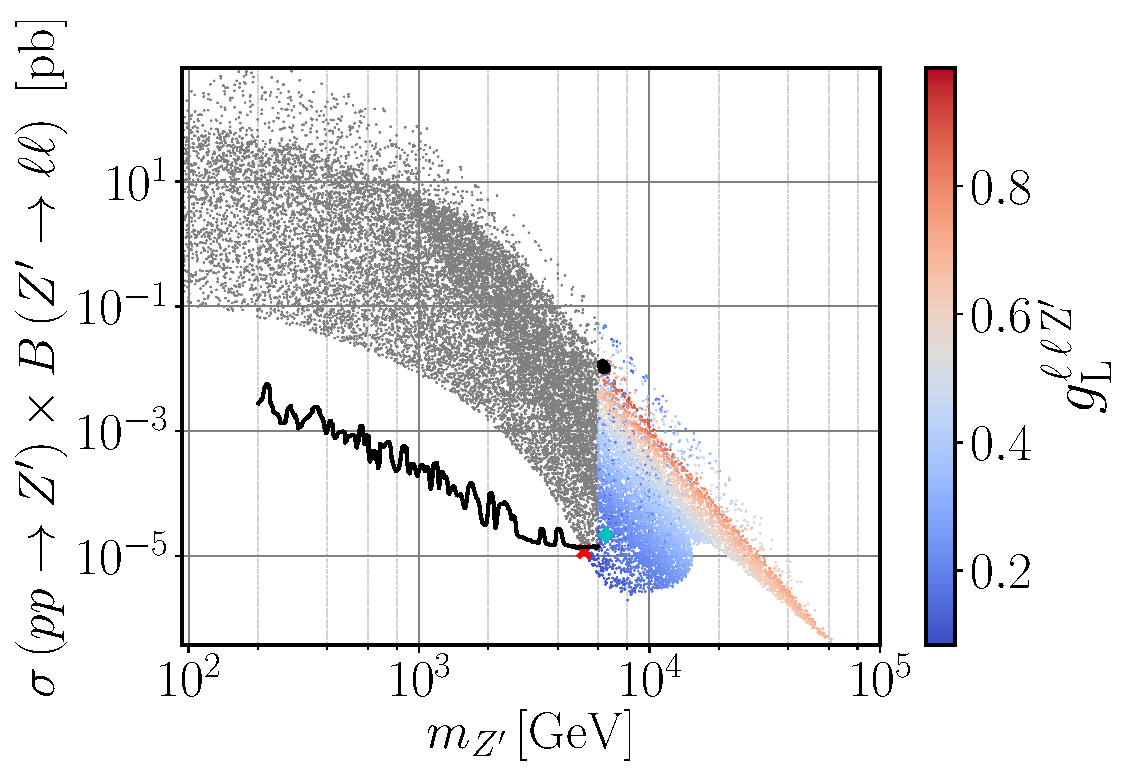
\includegraphics[scale=0.37]{Images/BLSM_2/mZp_Xsec_gLmumuZ.pdf}
	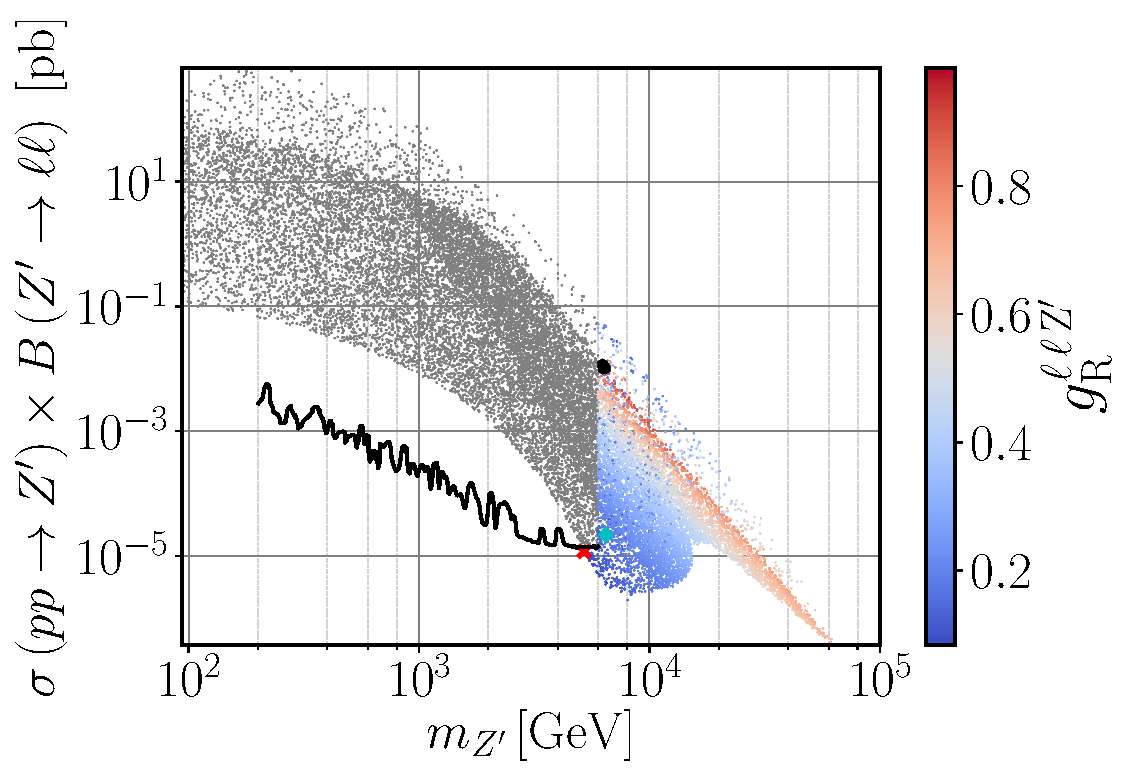
\includegraphics[scale=0.37]{Images/BLSM_2/mZp_Xsec_gRmumuZ.pdf}
	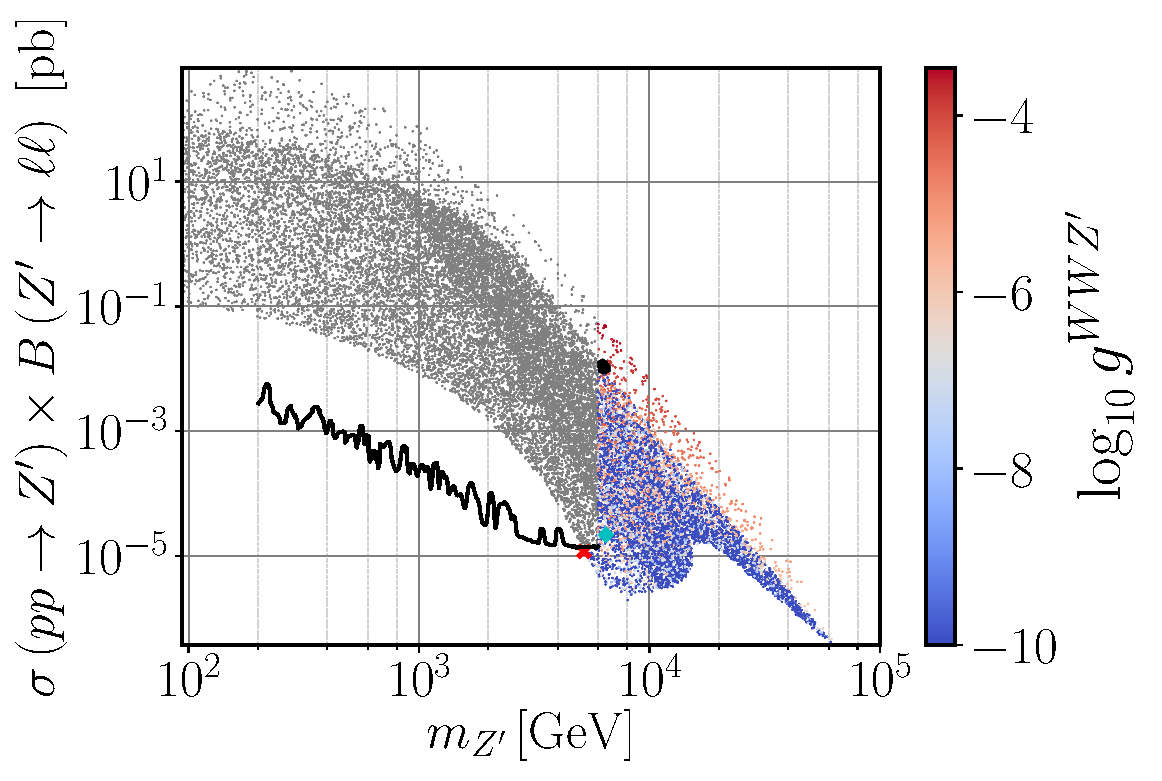
\includegraphics[scale=0.37]{Images/BLSM_2/mZp_Xsec_gWWZp.pdf}
    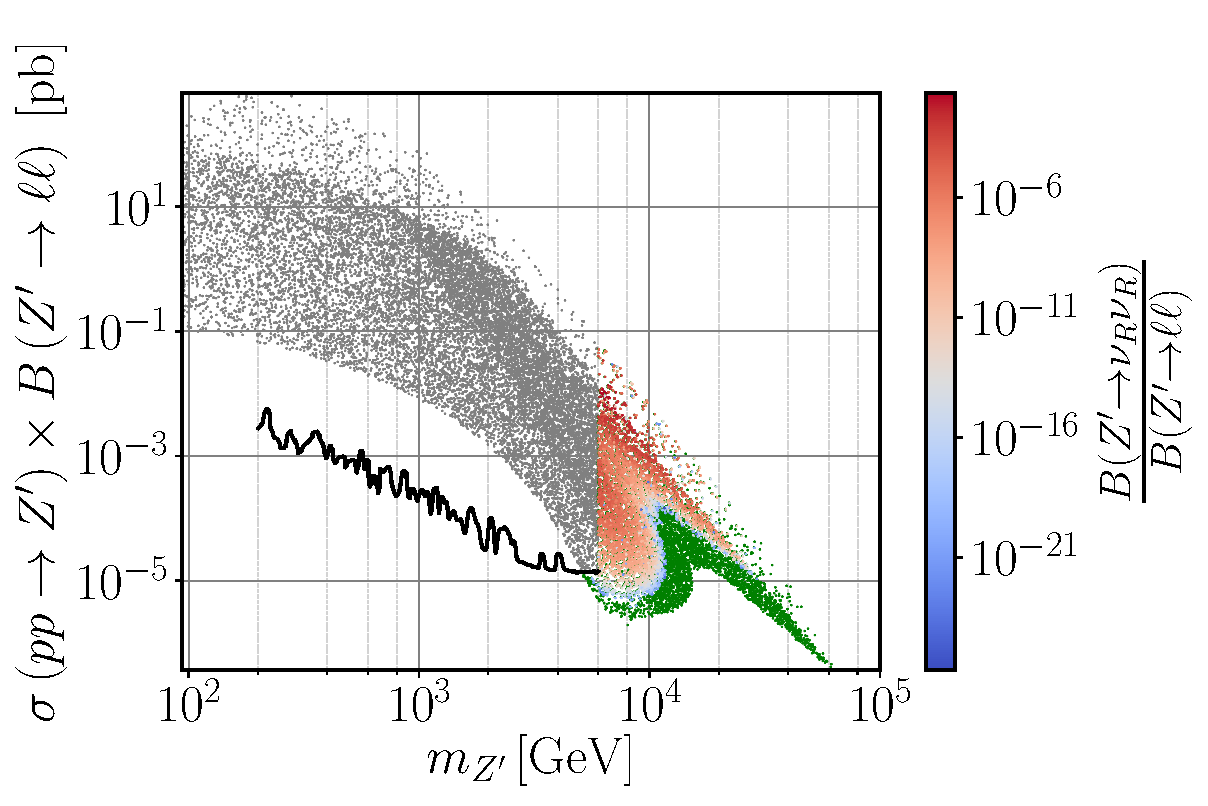
\includegraphics[scale=0.37]{Images/BLSM_2/Mzp_Xsec_zp_Neutr.pdf}
	\caption{The same as in Fig.~\ref{fig:Plots4} but with the colour scale representing the coupling of leptons to the $Z^\prime$ (top panels), 
	the coupling of $W$ bosons to $Z^\prime$ (bottom left) and the ratio of $Z^\prime$ branching 
	fraction to right-handed neutrinos $\nu_R$ over its branching fraction to charged leptons (bottom right). 
	In the bottom-right panel, green points correspond to allowed scenarios with fixed $B(Z^\prime \to \nu_R \nu_R)=0$. }
	\label{fig:Plots2}
\end{figure}	
%%%%%%%%%%%%%%%%%%%%%%%%%%

For completeness, we show in Fig.~\ref{fig:Plots2} the physical couplings of $Z^\prime$ to muons (top panels) and to $W^\pm$ bosons (bottom-left panel).
Note that, for the considered scenarios, the latter can be written as
\begin{equation}
    g^{WWZ^\prime} \simeq \dfrac{1}{16} \dfrac{\g{YB}{}}{\g{B-L}{}} \left(\dfrac{v}{x}\right)^2\,.
    \label{eq:gWWZp}
\end{equation}
While both $\g{B-L}{}$ and the ratio $v/x$ provide a smooth continuous contribution in the $\sigma B - m_{Z^\prime}$ projection of the parameter space, the observed blurry region in $g^{WWZ^\prime}$ is correlated with the one in the top-left panel of Fig.~\ref{fig:Plots3} as expected from Eq.~\eqref{eq:gWWZp}. On the other hand, the couplings to leptons $g_{\rm L,R}^{\ell \ell Z^\prime}$ exhibit a strong correlation with 
$\g{B-L}{}$ in Fig.~\ref{fig:Plots3} except for the sparser region on the upper edge of the $\sigma B - m_{Z^\prime}$ plane where the correlation becomes proportional to $\g{YB}{}$, in agreement with our discussion above and with Eqs.~\eqref{eq:gLgR-simp}. In the bottom-right panel of Fig.~\ref{fig:Plots2}, we have also shown the relative value of the $Z^\prime$ branching ratio into a pair of right-handed neutrinos, $B(Z^\prime \to \nu_R \nu_R)$, versus the corresponding branching fraction into charged leptons. We have found that the $Z^\prime$ decay into right-handed neutrinos is strongly suppressed for all the points that pass the theoretical and experimental constraints and thus cannot provide a significant impact on the exclusion bounds.

\subsubsection{Barr-Zee type contributions}
\label{sec:BarrZee}

To conclude our analysis, one should note that the two-loop Barr-Zee type diagrams \cite{Barr:1990vd} are always sub-dominant in our case. To see this, let us consider the four diagrams shown in Fig.~\ref{fig:Barr-Zee}.
%%%%%%%%%%%%%%%%%%%%%%%%%
\begin{figure}[!htb]
	\centering
	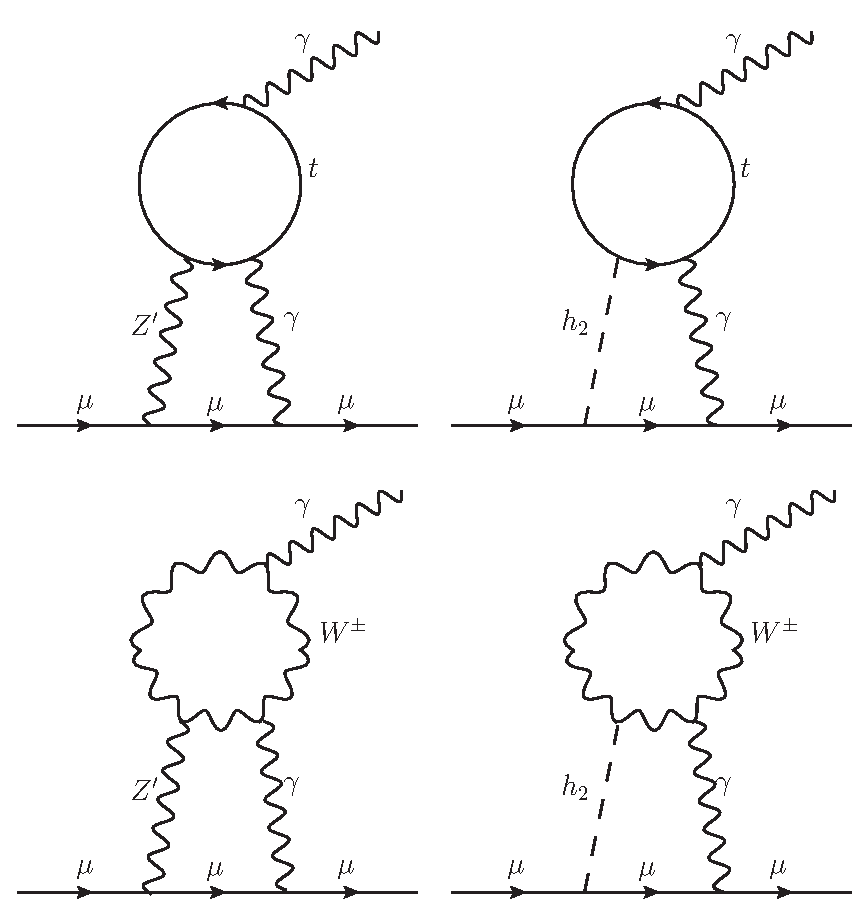
\includegraphics[scale=0.6]{Images/BLSM_2/Barr-Zee.pdf}
	\caption{Barr-Zee type two-loop diagrams contributing to $\Delta a_\mu$.}
	\label{fig:Barr-Zee}
\end{figure}	
%%%%%%%%%%%%%%%%%%%%%%%%%
The same reason that suppresses the one-loop $h_2$ contribution in Fig.~\ref{fig:g-2} is also responsible for the suppression of both the top-right and bottom-right diagrams in Fig.~\ref{fig:Barr-Zee} (for details see e.g.~Ref.~\cite{Ilisie:2015tra}). Recall that the coupling of $h_2$ to the SM particles is proportional to the scalar mixing angle $\alpha_h$, which is always small (or very small) as we can see in Fig.~\ref{fig:Plots4}. An analogous effect is present in the diagram involving a $W$-loop, where a vertex proportional to $g^{WWZ^\prime}$ suppresses such a contribution. The only diagram that might play a sizeable role is the top-left one where the couplings of $Z^\prime$ to both muons and top quarks are not negligible.

Let us then estimate the size of the first diagram in Fig.~\ref{fig:Barr-Zee}. This type of diagrams were already calculated in Ref.~\cite{Feng:2009gn} but for the case of a SM $Z$-boson. Since the same topology holds for the considered case of B-L-SM too, 
if we trade $Z$ by the new $Z^\prime$ boson, the contribution to the muon $(g-2)_\mu$ anomaly can be rewritten as
\begin{equation}
    \Delta a_\mu^{\gamma Z^\prime} = -\dfrac{g^2 \g{B-L}{2} m_\mu^2 \tan^2{\theta_W^\prime}}{1536 \pi^4} \left(g_{\ro{L}}^{ttZ^\prime} - g_{\ro{R}}^{ttZ^\prime}\right) {\ro{T}}_7\left( m_{Z^\prime}^2, m_t^2, m_t^2 \right)\,,
    \label{eq:agZ}
\end{equation}
where $g_{\ro{L,R}}^{ttZ^\prime}$, calculated in \texttt{SARAH}, are the left- and right-chirality projections of the $Z^\prime$ coupling to top-quarks, given by
\begin{equation}
\begin{aligned}
    g_{\ro{L}}^{ttZ^\prime} &= 
    - \dfrac{{\g{YB}{}}}{12} \cos{\theta_W^\prime}
    -\dfrac{\g{B-L}{}}{6} \cos{\theta_W^\prime} + \dfrac{g}{4} \cos{\theta_W} \sin{\theta_W^\prime} - \dfrac{\g{Y}{}}{12} \sin{\theta_W} \sin{\theta_W^\prime}\,,
    \\
    g_{\ro{R}}^{ttZ^\prime} &= 
    - \dfrac{\g{YB}{}}{3} \cos{\theta_W^\prime}
    -\dfrac{\g{B-L}{}}{6} \cos{\theta_W^\prime} - \dfrac{ \g{Y}{}}{3} \sin{\theta_W} \sin{\theta_W^\prime}\,.
\end{aligned}
\end{equation}
The loop integral $\ro{T}_7 \left(m_{Z^\prime}^2, m_t^2, m_t^2\right)$ was determined in Ref.~\cite{Feng:2009gn} and, in the limit $m_{Z^\prime} \gg m_t$, it gets simplified to,
\begin{equation}
    \ro{T}_7 \left(m_{Z^\prime}^2, m_t^2, m_t^2\right) \simeq \frac{2}{m_{Z^\prime}^2} \,,
    \label{eq:T7}
\end{equation}
up to a small truncation error. For the parameter space region under consideration the difference $g_{\ro{L}}^{ttZ^\prime} - g_{\ro{R}}^{ttZ^\prime}$ can be cast in a simplified form as follows 
\begin{equation}
    \left(g_{\ro{L}}^{ttZ^\prime} - g_{\ro{R}}^{ttZ^\prime}\right) \simeq \dfrac{1}{32} \g{YB}{} \left[ 8 + \dfrac{\left(g^2 + \g{Y}{2}\right)}{\g{B-L}{2}} \left(\dfrac{v}{x}\right)^2 \right] \approx \dfrac{1}{4} \g{YB}{} \,.
    \label{eq:gLminusgR}
\end{equation}
Using this result and the approximate value of the loop factor, we can calculate the ratio between 
the Barr-Zee type and one-loop contributions to the muon $(g-2)_{\mu}$,
\begin{equation}
    \dfrac{\Delta a_\mu^{\gamma Z^\prime}}{\Delta a_\mu^{Z^\prime}} \simeq -\dfrac{1}{4096 \pi^2}\dfrac{g^2 \left(g^2 + \g{Y}{2}\right) \g{YB}{3}}{\left[6 \g{B-L}{} \g{YB}{}  + 4\g{B-L}{2} + \g{YB}{2} \right] } \left(\dfrac{v}{x}\right)^4 \ll 1 \,,
\end{equation}
which shows that $\Delta a_\mu^{\gamma Z^\prime}$ does indeed play a subdominant role in our analysis and can be safely neglected.

\chapter{3HDM Model}
\label{ch:3HDM}

As already mentioned, in this chapter we specialize our analysis tools and methodology to the case of a less minimal model. In particular, we study a three Higgs Doublet Model (3HDM), supplemented with a BGL-like (Branco-Grimus-Lavoura) structure, characterized by a $\mathrm{U}(1) \times \mathbb{Z}_2$ global flavor symmetry, such as presented in Refs.~\cite{Ludvig_Thesis,Ian_Thesis}. Such a symmetry was engineered to suppress Higgs mediated flavour violating interactions. Note that, as mentioned in the introduction, without this symmetry these processes, which typically occur at tree-level in multi-Higgs Models, would contradict observations. Furthermore, in our model it will completely forbid quark FCNCs in the up-sector. 

The structure of this chapter will consist in first, introducing the BGL-like 3HDM and then  performing a numerical analysis in a similar fashion as for that the B-L-SM. However, the new simulations use an updated version of the previously discussed code featuring the addition of a public flavour physics calculation tool entitled \texttt{flavio} \cite{straub2018flavio}. 

A key change from the B-L-SM case is, however, that the respective masses will all be calculated at tree-level instead of at 2-loop level. This is done for multiple reasons, most of which reflect computational and formal difficulties, time constraints, and, above all, that it is not relevant for our current purposes. Note that radiative processes are still calculated just using tree-level masses, e.g. the values of the STU oblique parameters are still calculated by SPheno at one loop-order but for a tree-level set of masses.   

Let us mention that BGL models are typically known in the context of 2HDMs (such as in ,\cite{Branco_1996}). The idea is to impose symmetries that naturally keep FCNCs under control through the CKM matrix. Several phenomenology studies where previously done in 2HDMs (see \cite{Botella_2016}), however this type of studies are still somewhat novel for 3HDMs. Furthermore, besides a different phenomenology, it is agreed that 3HDM contain some advantages. To name a few, they can provide more than one stable source of spontaneous $\mathcal{CP}$-breaking and charge breaking minima are found to be stable while at the same time coexisting with the charge preserving ones (for more information see, \cite{Barroso_2006}). 

\begin{comment}

\section{The Case of the BGL-2HDM and its Relation to our Work}

Any 3HDM can be thought of as part of a larger family of multiple Higgs Doublet Models, or NHDMs, the first iteration of which was the Two Higgs Doublet Model (2HDM) proposed by T.D. Lee \cite{Lee1973}. At the time, Lee was motivated by the search for a spontaneous breaking of the $\mathcal{CP}$ symmetry which was included in his model.  However the 2HDM quickly became a very popular model because of its inclusion of dark matter candidates, as well as providing a large particle spectrum, able to be discovered in collider, which also led to the inclusion charged and additional neutral scalars who enable FCNC deviations. In spite of the fact that, now, these tree-level FCNCs are in direct opposition to experimental results, as discussed in section \ref{Chap_1_Sec_3}. Given these limits and the models popularity, we can consult the literature, as in Ref. \cite{Branco:1999fs}, and see that the existence of FCNCs forces the extra scalars in the minimal 2HDM case to have masses above 1 TeV as to suppress FCNCs. These heavy scalars are far from ideal, since there is no indication such heavy scalars exist nor do they provide us with interesting physics. 

Several mechanisms have been proposed to act as a suppression of these tree-level FCNCs, to then allow for richer physics and lighter scalars. First, in Ref. \cite{ferreira2019strong}, it is proposed a framework in which we have the balancing of $\mathcal{CP}$-odd and $\mathcal{CP}$-even contribution to FCNCs, however, this requires some fine-tuning, making it very unappealing based on a ``naturalist" argument. Another possibility is to assume alignment between different Yukawa matrices such that no FCNCs are present, see \cite{Jung_2011}. Finally we could also use the approach presented in the BGL version of the 2HDM \cite{Branco_1996}, here the authors impose a flavor-violating symmetry naturally keeping the FCNCs under control through the CKM matrix. The phenomenology of the model has been studied quite thoroughly in previous works, see Ref. \cite{Botella_2016}, and it remains a possible scenario for BSM physics.

As the name indicates, NHDMs, are types of models where, in parallel with the standard SM Higgs doublet some additional replicas of that same  (or slightly modified) doublet are introduced. In the NHDM these form a sort of family in the scalar sector in analogy to the fermion sector. Being that the 3HDM is the most similar. This idea is far from original and was first discussed by Weinberg in Ref. \cite{Weinberg1976}.

Phenomenologically speaking these 2HDMs and 3HDMs models are quite different however, and we can argue that there are several advantages to the 3HDM. Such as, unlike in the 2HDM case, the 3HDM can provide more than one stable source of spontaneous CP symmetry breaking \cite{Branco_2012}. Furthermore, charge breaking minima were found to be stable while at the same time coexisting with charge-preserving ones (for more information see, \cite{Barroso_2006}). Note also, for the 2HDM a full list of all possible incorporation of symmetries consistent with $\mathrm{SU(2)}\times\mathrm{U(1)}$ has been achieved \cite{Ivanov_2008}, while for the 3HDM no work has thus far been completed, see, \cite{Ivanov_2015}. Although in this work, we do not include imaginary potential terms that would lead to additional $\mathcal{CP}$-violation. 

Instead, we explore a 3HDM with a global flavor symmetry to replicate the BGL treatment. Similar studies have been done in 3HDMs that include different flavor symmetries, such as Ref.\,\cite{Camargo_Molina_2018}. Given the 3HDMs  background it is no surprise that we will focus particularly in the measuring Quark Flavor Violation (QFV) observables. In our analysis these will consist of meson decays or oscillations that include the changing of quark flavor within the meson. These QFV observables will be compared to measured amplitudes in collider experiments as to offer a novel exclusion to our model. Note, the additional flavor symmetry constrains the terms that can appear in the Yukawa sector of the Lagrangian resulting in very specific structures (or textures) of the Yukawa couplings. These shapes generate a suppression mechanism through the CKM matrix off-diagonal terms restricting the values of FCNCs in our model.%

\end{comment} 

\section{The formulation of a BGL-like 3HDM} 
Let us start by reviewing the theoretical details necessary for our numerical analysis. These have initially been discussed in \cite{Ian_Thesis} and will be updated in this thesis and in \cite{Future}. Again, for this model, we still retain most of the same fields as in the SM, chapter~\ref{Chap:SM}, with the addition of two extra Higgs doublets. These fields are seen in, 
%
\begin{equation}
\label{eq:3HDM_Fields}
\begin{gathered}
Q_{L_i} =  \begin{pmatrix}
u_{L_i}  \\
d_{L_i}
\end{pmatrix} \quad , \quad \Psi_{L_i} =  \begin{pmatrix}
\nu_{L_i}  \\
e_{L_i}
\end{pmatrix}  ,  \\ 
p_R \quad , \quad n_R \quad , \quad e_{R_i} \quad i=\{1,2,3\}  ,  \\  
\phi_k = \begin{pmatrix}
  W_k^+ \\ 
\frac{1}{\sqrt{2}}\left( v_k + h_k + i Z_k \right) 
\end{pmatrix}  \quad , \quad k=\{ 1,2,3\}  . 
\end{gathered} 
\end{equation}
%
where $Q_{L_i}$ , $\phi_k$ and $\Psi_{L_i}$ are $\mathrm{SU(2)_L}$ doublets fields, while, $p$ and $n$ (analogous to $u_{R_i}$, $d_{R_i}$ in the SM ), and $e_{R_i}$ are $\mathrm{SU(2)_L}$ singlets where the i and k generation stand for their respective generation indexes. Note that $p$ and $n$ stand for positive and negative quarks, respectively. The new quantum numbers under $\mathrm{U(1)}\times\mathbb{Z}_2$ can be seen in the transformations that these fields undergo, 
%
\begin{equation}
\label{eq:3HDM_Transformations}
\begin{split} 
\mathrm{U(1)} : & \\
& Q_{L_3} \rightarrow    e^{i \alpha} Q_{L_3}  \\  
& p_{R_3} \rightarrow    e^{2 i \alpha} p_{R_3}  \\
& \phi_1  \rightarrow    e^{i \alpha} \phi_1  \\   
& \Psi_{L_1} \rightarrow e^{i \alpha} \Psi_{L_1} \\
& \phi_3 \rightarrow     e^{i \alpha} \phi_3  \\ 
\end{split} \quad \quad \quad  
\begin{split}
\mathbb{Z}_2 : & \\
& Q_{L_3} \rightarrow -Q_{L_3} \\
& p_{R_3} \rightarrow -p_{R_3} \\ 
& \phi_1  \rightarrow -\phi_1 \\ 
& \Psi_{L_1} \rightarrow - \Psi_{L_1} \\ 
& \phi_3 \rightarrow -\phi_3
\end{split}  
\end{equation} 
%
All remaining fields not shown in Eq.~(\ref{eq:3HDM_Transformations}) remain unchanged under transformations of the $\mathrm{U(1)}\times\mathbb{Z}_2$ global symmetry i.e.\,are not charged under these symmetries.  
%
Note there is no right handed neutrino fields in this model making it so that no neutrino mass terms appear unlike in the case of the B-L-SM previously studied.

\subsection{The Scalar Sector}

Let us then start by introducing the scalar sector where the new spin-0 $\mathrm{SU(2)}$ doublets, $\phi_k$, $k=\{1,2,3\}$ reside.
%
Note the scalar potential is $\mathcal{CP}$-invariant, this means, 
%
\begin{equation}
\phi_1 = \phi_1^{\**} \quad , \quad \phi_2 = \phi_2^{\**} \quad , \quad 
\phi_3 = \phi_3^{\**} . 
\end{equation}
and that all other parameters in the potential in Eq.~(\ref{eq:3HDM_Scalar_Pot}), such as $(\lambda_i,i=\{1,...,10\})$ and soft-breaking terms ($\mu_{i}$ $i=\{1,2,3\}$, $\mu_{21}$,$\mu_{13}$ and $\mu_{23}$) are real.  
%
The generic scalar potential is extensively written as, 
\begin{equation}
\label{eq:3HDM_Scalar_Pot}
\begin{split}
V(\phi_i) = & 
- \mu_1^2 \left( \phi^{\dagger}_1 \phi_1 \right) 
- \mu_2^2 \left( \phi^{\dagger}_2 \phi_2 \right)  
- \mu_3^2 \left( \phi^{\dagger}_3 \phi_3 \right) \\ 
& \left[ - \mu_{21}^2 \left( \phi^{\dagger}_2 \phi_1  \right) 
- \mu_{23}^2 \left( \phi^{\dagger}_2 \phi_3  \right)  
- \mu_{13}^2 \left( \phi^{\dagger}_1 \phi_3  \right) + \text{H.c.} \right]  \\
& + \lambda_1 \left( \phi^{\dagger}_1 \phi_1 \right)^2 
+ \lambda_2 \left( \phi^{\dagger}_2 \phi_2 \right)^2  
+ \lambda_3 \left( \phi^{\dagger}_3 \phi_3 \right)^2 \\  
& + \lambda_4 \left( \phi^{\dagger}_1 \phi_1 \right)  \left( \phi^{\dagger}_2 \phi_2 \right) 
+ \lambda_5 \left( \phi^{\dagger}_1 \phi_1 \right)  \left( \phi^{\dagger}_3 \phi_3 \right)  
+ \lambda_6 \left( \phi^{\dagger}_2 \phi_2 \right)  \left( \phi^{\dagger}_3 \phi_3 \right)  \\ 
& + \lambda_7 \left( \phi^{\dagger}_1 \phi_2 \right)  \left( \phi^{\dagger}_1 \phi_2 \right)  
+ \lambda_8 \left( \phi^{\dagger}_1 \phi_3 \right)  \left( \phi^{\dagger}_3 \phi_1 \right)   
+ \lambda_9 \left( \phi^{\dagger}_2 \phi_3 \right)  \left( \phi^{\dagger}_3 \phi_2 \right)  \\
& + \lambda_{10} \Bigg\{ \left( \phi^{\dagger}_1 \phi_3 \right)^2 + \text{H.c.} \Bigg\} . 
\end{split} 
\end{equation}
%
The most generic version of the soft breaking of the imposed flavour symmetry is given by the second line, where the terms $\mu_{23}^2$, $\mu_{13}^2$ and $\mu_{21}^2$ are seen. 
%
The parameters are necessarily added as to impede the formation of a massless axion. Note that the only term that respect the $\mathbb{Z}_2$ symmetry is $\mu_{13}$ while the others explicitly break it. Also the $\mathrm{U(1)}$ symmetry is broken explicitly by all these terms. 

After the process of SBB, all Higgs doublets, $\phi_k$, develop a VEV  similar to that of the SM Higgs, written as, 
%
\begin{equation}
\phi_k = 
\begin{pmatrix}
W_k^\pm + i \, W_k^\mp \\ 
\frac{1}{\sqrt{2}}\left( v_k + h_k + i Z_k \right)
\end{pmatrix}  \rightarrow \langle \phi_k \rangle = \begin{pmatrix}
0 \\ 
\frac{v_k}{\sqrt{2}}
\end{pmatrix} \quad , \quad k=\{ 1,2,3\} .  
\label{eq:3HDM_Higgs_Field_VEV} 
\end{equation} 
%
Here we see the charged components of the field, $W_k^\pm$, the $\mathcal{CP}$-odd degree of freedom, $Z_k$, and finally the $\mathcal{CP}$-even fields, $h_k$. The scalar potential is minimized by the so called tadpole equations, these read as, 
%
\begin{equation}
\label{eq:3HDM_tadpoles}
\begin{gathered}
\frac{\partial V}{\partial \phi_1} =  \frac{1}{2} v_1 \left(-2 \mu _1^2+\left(\lambda _4+\lambda _7\right) v_1^2+\left(\lambda _5+\lambda _8+2 \lambda _{10}\right) v_7^2\right)+\lambda _1 v_1^3-\mu _{13}^2 v_3-\mu _{21}^2 v_2 = 0 \\ 
\frac{\partial V}{\partial \phi_2} =  \frac{1}{2} v_2^2 \left(-2 \mu _2^2+\left(\lambda _6+\lambda _9\right) v_3^2+\left(\lambda _4+\lambda _7\right) v_1\right)+\lambda _2 v_2^3-\mu _{21}^2 v_1-\mu _{23}^2 v_3  = 0 \\
\frac{\partial V}{\partial \phi_3} =  \frac{1}{2} \left(2 \lambda _3 v_3^3+\left(\lambda _6+\lambda _9\right) v_2^2 v_3+\left(\lambda _5+\lambda _8+2 \lambda _{10}\right) v_1^2 v_3-2 \mu _3^2 v_3-2 \mu _{13}^2 v_1-2 \mu _{23}^2 v_2\right)  = 0 \, . \\
\end{gathered} 
\end{equation}

\subsubsection{The Higgs Basis}

It is convenient for the remainder of our study to now introduce the basis changing matrix to what we will call the Higgs Basis. In our analysis of the 3HDM we did not perform the conventional direct diagonalisation of the scalar, Gauge and Yukawa bi-linear terms expressed in the scalar potential (Eq.\,(\ref{eq:3HDM_Scalar_Pot})) expanded around the vacuum state. Instead we use an intermediate basis as to significantly simplify the analysis of the scalar, pseudoscalar, charged scalar and quark physical terms 

The transformation from the gauge to the Higgs basis reads, 
\begin{equation}
\mathcal{O} = 
\begin{pmatrix}
\dfrac{v}{v_1} & \dfrac{v}{v_2}  & \dfrac{v}{v_3} \\[1.2em]
\dfrac{v_3}{v_{13}} & 0 & \dfrac{-v_1}{v_{13}} \\[1.2em]
\dfrac{v_2 v_1}{v v_{13}}  & \dfrac{v_{13}}{v} & \dfrac{v_2 v_3}{v v_{13}}  
\end{pmatrix} , 
\end{equation}
%
where $v_{13}=\sqrt{v_1^2 + v_3^2}$ and $v=\sqrt{v_1^2 + v_2^2 + v_3^2 }$, the total magnitude. This basis transformation explicitly relates the fields in the following manner, 
%
\begin{equation}
\begin{pmatrix}
\phi_1 \\
\phi_2 \\
\phi_3 \\
\end{pmatrix} = 
\mathcal{O} \begin{pmatrix}
h \\
H_1^\prime \\
H_2^\prime \\
\end{pmatrix} 
%
\quad , \quad 
%
\begin{pmatrix}
Z_1 \\
Z_2 \\
Z_3 \\
\end{pmatrix} = 
\mathcal{O} \begin{pmatrix}
z \\
A_1^\prime  \\
A_2^\prime  \\
\end{pmatrix} 
%
\quad , \quad 
%
\begin{pmatrix}
W_1^\pm  \\
W_2^\pm  \\
W_3^\pm  \\
\end{pmatrix} = 
\mathcal{O} \begin{pmatrix}
\omega^\pm \\
H_1^{\pm \prime}  \\
H_2^{\pm \prime}  \\
\end{pmatrix} . 
\end{equation}
%
These VEVs can also be parameterized through their mixing. 
\begin{equation}
v_1 = v \cos(\psi_1) \cos(\psi_2) \quad , \quad v_2 = v \sin(\psi_1) \cos(\psi_2) \quad , \quad v_3 = v \sin(\psi_2) , 
\end{equation}
%
where the two mixing angles are $\psi_1$ and $\psi_2$. 
%
Through this we can re-write the orthogonal mixing matrix, 
%
\begin{equation}
\label{eq:3HDM_Orthg}
\mathcal{O} = 
\begin{pmatrix}
\cos(\psi_1) \cos(\psi_2) & \sin(\psi_2) & \cos(\psi_2) \sin(\psi_1)   \\ 
\cos(\psi_1) & 0 & - \sin(\psi_1)  \\ 
- \sin(\psi_1) \sin(\psi_2) & \cos(\psi_2) &  \cos(\psi_1) \sin(\psi_2)
\end{pmatrix} . 
\end{equation}

For now let us take a small pause and perform the diagonalization of the Higgs eigenstates in a later time.  

\subsection{The Gauge Sector}

%Before beginning our study of the inversion process of the scalar sector it is prudent to first consider and discuss the remaining portions of the 3HDM Lagrangian. 
%
We begin by presenting the Gauge sector. 
%
Note, after the Higgs Doublets shift to their VEVs and we write the Lagrangian terms with their physical fields, the gauge interactions read as,  
%
\begin{equation}
\mathcal{L}_{\text{gauge}} \supset \frac{1}{4} \left( v_1^2 + v_2^2  + v_3^2 \right) g^2 W^+_\mu W^{-\,\mu} + \frac{1}{8} \left(  v_1^2 + v_2^2  + v_3^2  \right) \left( g^{\prime \, 2} + g^2 \right) Z_\mu Z^\mu  .
\end{equation}
%
We can clearly see that to reproduce the correct gauge boson masses we must ensure that,
%
\begin{equation}
\label{eq:VEV_Condition}
\sum_{k=1}^3 v_k^2 \approx 246^2 \ \text{(GeV)}^2  . 
\end{equation}
%
This condition constraints the range of values that the Higgs doublet VEVs can take. 

Recall that the couplings to the Higgs boson to vector bosons and heavier fermions have also been precisely measured meaning that the only way to comply with current experimental constraints is to have a state that behaves very similarly with the observed Higgs boson with the measured mass of 125.09 GeV.  This is why we impose the previously mentioned Higgs alignment limit.  This is explicitly demonstrated in Ref.~\cite{das2015implications}.  

This alignment then consists in a particular configuration of the 3HDM parameter space such that one of the Higgs states in the gauge basis completely overlaps with the physical one i.e.\,completely aligned with the $\mathcal{CP}$-even physical Higgs boson ($h$). 
%
In our case the alignment limit is particularly convenient in order to reproduce the same SM-like Leptonic Yukawa sector, as in the SM, provided that they couple exclusively to this SM-like Higgs.
%
This means that our 3HDM is lepton flavour universal just like the SM. Note that a strict alignment is not manifestly required by the data and in fact there are ways we could deviate as much as $\mathcal{O}(10\%)$ (see Ref.\,\cite{Aad_2020}) from the SM predicted gauge coupling value through a small mixing. 
%
However our purpose in the current analysis is to show that our BGL-like symmetry can indeed control tree-level FCNCs. Any deviation from alignment would not strongly affect our main message but would have an scan efficiency cost. Such extension is left for future work. 


\subsection{The Yukawa sector}

Now having dealt with the gauge sector and introduced the concept of Higgs alignment we can continue to study the Yukawa sector. The 3HDM Yukawa interactions read as,
%
\begin{equation} 
\label{eq:3HDM_Yuk} 
\begin{split} 
\mathcal{L}_Y = - & \sum_{k=1}^3 \left[ \overline{Q}_{L_a} \left( \Gamma_k \right)_{ab} \phi_k n_{R_b} + \overline{Q}_{L_a} \left( \Delta_k \right)_{ab} \tilde{\phi}_k p_{R_b} + \text{H.c}.  \right] \\ + & \left( \Psi_{L_a} \left( Y^e_1 \right)_{ab} \phi_1 e_{R_b} + \text{H.c} \right) .
\end{split} 
\end{equation} 
%
Here, $\Gamma_k$ and $\Delta_k$ are the down and up Yukawa matrices in the 3HDM model respectively, one for each, $k$, Higgs doublet. 
%
Consider that the shape of this Yukawa sector is very similar to the SM Yukawa sector but for more Higgs doublets. Furthermore, notice how the leptons couple only to the first generation Higgs Doublet, as previously stated. 
%
This translates into the lepton Yukawa matrix being diagonal as in the SM, and preserving lepton flavour universality, 
%
\begin{equation}
Y_e = \frac{\sqrt{2}}{v_1} M_{\text{diag.}}\left( m_e , m_\mu , m_\tau \right) .
\end{equation} 
%
Let us then examine the effects the imposed symmetry, $\mathrm{U}(1)\times\mathbb{Z}_2$, has on the Yukawa matrices, showing us their textures.  
%
\begin{equation}
\begin{aligned}
\label{Lovely_Equations}
&\Gamma_1  = \begin{pmatrix}
0 & 0 & 0\\
0 & 0 & 0\\
\times & \times & 0
\end{pmatrix}, \quad 
&&\Gamma_2  = \begin{pmatrix}
\times & \times & 0\\
\times & \times & 0\\
0 & 0 & 0
\end{pmatrix}, \quad
\Gamma_3  = \begin{pmatrix}
0 & 0 & 0\\
0 & 0 & 0\\
0 & 0 & \times
\end{pmatrix}, \\[1em]
&\Delta_1  = \begin{pmatrix}
0 & 0 & 0\\
0 & 0 & 0\\
0 & 0 & 0
\end{pmatrix}, \quad 
&&\Delta_2 = \begin{pmatrix}
\times & \times & 0\\
\times & \times & 0\\
0 & 0 & 0
\end{pmatrix} , \quad 
\Delta_3 = \begin{pmatrix}
0 & 0 & 0\\
0 & 0 & 0\\
0 & 0 & \times
\end{pmatrix}  \, . 
\end{aligned} 
\end{equation}
%
Here the $\times$ represent a complex non-zero value in the respective matrix. 
%
We can immediately see the treatment of the first generation of quarks differ between down and up types.  And that within the up and down type matrices there is no overlap of matrix elements.  
% 
The quark masses in the flavour (or gauge) eigenbasis have the following form,
\begin{equation}
\label{eq:3HDM_Quark_gauge_mass}
\begin{split}
M_n = \frac{v_1}{\sqrt{2}} \Gamma_1 +  \frac{v_2}{\sqrt{2}} \Gamma_2 +  \frac{v_3}{\sqrt{2}} \Gamma_3  \quad , \\ 
M_p = \frac{v_1}{\sqrt{2}} \Delta_1 +  \frac{v_2}{\sqrt{2}} \Delta_2 +  \frac{v_3}{\sqrt{2}} \Delta_3   \quad .
\end{split}
\end{equation}
%
Here we begin to notice the origin of the tree-level FCNCs in 3HDMs given the Yukawa textures. We observe the following mass terms in the gauge basis, 
%
\begin{equation}
M_n = \begin{pmatrix}
\times & \times & 0 \\
\times & \times & 0 \\
0 & 0 & \times 
\end{pmatrix} 
\quad , \quad 
M_p=\begin{pmatrix}
\times & \times & 0 \\
\times & \times & 0 \\
\times & \times & \times 
\end{pmatrix} .
\end{equation}
%
In order to study this sector we must be able to transform the $n$ and $p$ into their physical quark fields $d$ and $u$ respectively. 
%
This, like in the SM, is achieved by a set of bi-unitarity transformations, $V_{L,R}$ and $U_{L,R}$, where the CKM matrix will be $V_{\text{CKM}} = V_L^\dagger U_L$. These matrices are defined as, 
%
\begin{equation}
%\begin{split}
m_u^{\text{diag}} = V_L^n M_n V_R^n \equiv V_L^n \begin{pmatrix}
\times & \times & 0 \\
\times & \times & 0 \\
0 & 0 & \times 
\end{pmatrix}  V_R^n  \quad , \quad 
m_d^{\text{diag}} = U_L^p  M_p U_R^p \equiv U_L^p \begin{pmatrix}
\times & \times & 0 \\
\times & \times & 0 \\
\times & \times & \times \\ \end{pmatrix} U_R^p . 
%\end{split} 
\end{equation}
The relations between these gauge eigenstates ($n$ and $p$) and mass basis states ($u$ and $d$) are, 
\begin{equation}
\label{3HDM_states}
p_L = V_L u_n \quad , \quad p_R = V_R u_R \quad , \quad n_L = U_L d_L \quad , \quad n_R = U_R d_R \, .
\end{equation}
This then imposes certain shapes on the unitary transformations. 
\begin{equation}
V^{n}_{L} = \begin{pmatrix}
\times & \times & 0 \\ 
\times & \times & 0 \\
0 & 0 & 1 \\ 
\end{pmatrix} \quad , \quad   V^{n}_{R} = \begin{pmatrix}
\times & \times & 0 \\ 
\times & \times & 0 \\
0 & 0 & e^{i\alpha}  \\ 
\end{pmatrix}  \quad , \quad 
U^{p}_{L,R} = 
\begin{pmatrix}
\times & \times & \times \\ 
\times & \times & \times \\
\times & \times & \times \\
\end{pmatrix} .
\end{equation}
Several conventions are possible but we choose to  introduce a complex phase in $V^n_{L,R}$ so that these matrices can be parametrized with two angles. While the parametrization of $U^p_{L,R}$ will require 3. We know these to be the physical degrees of freedom that will be included in the CKM matrix. The CKM matrix elements can then be expressed as, 
\begin{equation}
\begin{gathered}
V_{CKM} = V_L^n U_L^{p\, \dagger}  \ , \\ 
\\
\begin{pmatrix}
V_{ud} & V_{us} & V_{ub} \\
V_{cd} & V_{cs} & V_{cb} \\ 
V_{td} & V_{ts} & V_{tb} 
\end{pmatrix}  = \begin{pmatrix}
V_{L,11}^n & V_{L,12}^n & 0 \\ 
V_{L,21}^n & V_{L,22}^n & 0 \\ 
0 & 0 & e^{i \alpha} 
\end{pmatrix} \begin{pmatrix}
U_{L,11}^p & U_{L,12}^p & U_{L,13}^p \\
U_{L,21}^p & U_{L,22}^p & U_{L,23}^p \\
U_{L,31}^p & U_{L,32}^p & U_{L,33}^p \\
\end{pmatrix} ^\dagger \ .
\end{gathered} 
\end{equation}
%
These equations allow for a system of coupled linear equations that can be solved with respect to the Yukawa textures given a set of physical inputs such as quark masses and CKM mixing. 
%
With this convention we can see that, up to a phase $\alpha$, the last row $V^p_L$ is completely determined by the CKM matrix.
%
Therefore, by defining the simple projection operator, $P$, 
%
\begin{equation}
P = 
\begin{pmatrix}
0 & 0 & 0 \\ 
0 & 0 & 0 \\ 
0 & 0 & 1 
\end{pmatrix}. 
\end{equation}
We are capable of extracting this last row. With this parameterization we are able to use quark masses and the CKM mixing as inputs of our scan instead of fitting them. Such a procedure significantly boosts the efficiency of our scan. 

\section{The BGL-like suppression of FCNCs in the 3HDM model}

Given what we know now we can look at the case of FCNCs present in the model and the role of the BGL-like mechanism. 
%
We expect that $\phi_1$ generates no tree-level FCNCs given its full overlap with the SM Higgs boson. 
%
However, heavier non-SM states feature tree-level FCNCs. This can severely constrain our model unless the couplings of BSM-scalars to the SM are small enough to compensate such a tree-level effect. This is the motivation behind the BGL treatment as discussed. 

To illustrate how this mechanism works, we show the FCNC contributions of the $\mathcal{CP}$-even states, $H_1^\prime$ and $H_2^\prime$.
%
Let us then look at the rotated Yukawa interactions. 
%
\begin{equation}
\mathcal{L}^{H_1^\prime \, , \, H_2^\prime}_Y = 
\frac{H_1^\prime}{v} \overline{n}_L N_{d\,1} n_R + 
\frac{H_2^\prime}{v} \overline{n}_L N_{d\,2} n_R + 
\text{H.c.} \ . 
\end{equation} 
% 
where the matrix terms $N_{d\,1}$ and $N_{d\,2}$ can be shown to lead us to, Eq.\,(\ref{Eq:3HDM_:)}) through the use of Eq.~(\ref{3HDM_states}).   
\begin{equation}
\label{Eq:3HDM_:)}
\begin{split}
N_{d\,1} = & \frac{v}{\sqrt{2} v_{13}} V_L^{n \, \dagger} \left( \Gamma_1 v_3 - \Gamma_3 v_1 \right) V_R^{n} \ , \\ 
N_{d\,2} = & V_L^{n \dagger} \left[ \frac{v_2}{v_{13}} \frac{1}{\sqrt{2}} \left( \gamma_1 v_1 + \gamma_3 v_3 \right) - \frac{v_{13}}{v_2} \frac{1}{\sqrt{2}} \Gamma_2 v_2  \right] V_R^n \ . 
\end{split} 
\end{equation}
We can now simplify Eq.~(\ref{Eq:3HDM_:)}) using the textures of the Yukawas matrices in Eq.~(\ref{Lovely_Equations}). Keeping the third row of $U_L$ the same as the \text{CKM} matrix, we can write the down sector Yukawa matrices as: 
%in the down sector sector Yukawa matrices write, 
\begin{equation}
\Gamma_3 = (\Gamma_3)_{33} P \quad , \quad \frac{1}{\sqrt{2}}  \left( \Gamma_1 v_3 - \Gamma_3 v_1 \right) =  P M_d \ .  
\end{equation}
Hence, 
\begin{equation}
\begin{split}
(N_{d\,1})_{ij} = & \frac{v v_3}{v_1 v_{13}} (V_{\text{CKM}}^\**)_{3i} V_{\text{CKM}}^{3j} (M_d)_{jj} - \frac{1}{\sqrt{2}} \frac{v v_{13}}{v_1} ( \Gamma_3 )_{33} (V_{CKM}^{\**})_{3i} (V_R^n)_{3j},  \\ 
(N_{d\,2})_{ij} = & \frac{v_{13}}{v_2} ( M_d )_{jj} \delta_{ij} + \left( \frac{v_{13}}{v_2} + \frac{v_2}{v_{13}} \right) (V^{\**}_{\text{CKM}})_{3i} V_{\text{CKM}}^{3j} (M_d)_{jj}. 
\label{Eq:3HDM_self_;)}
\end{split} 
\end{equation}
%
We can see in Eq.\,(\ref{Eq:3HDM_self_;)}), that all non diagonal terms of $N_{d\,2}$, ($j \neq i$) where FCNC are mediated, contain two CKM matrix terms, while for $N_{d\,1}$ we have one CKM matrix elements. Even given these terms we must suppress the size of the elements in $\Gamma_3$, and in order to further control FCNC interactions. 

A similar procedure in the up quark sector would reveal that there are no scalar mediated FCNCs at tree level. 

%
This is due to the special structure of the up type Yukawa matrices, which can be simultaneously diagonalized thus forbidding tree-level FCNCs. 
%
This is a consequence of the flavour symmetry. 

\section{The inversion procedure for scalars}

Over the course of this chapter we have alluded to the Higgs alignment limit such that one of the physical scalars completely overlaps with a SM-like Higgs. To ensure this in our data we must apply an inversion procedure and require the alignment limit as an input. With an inversion procedure, it should be possible to express all Lagrangian parameters with respect to physical observables, such as mixing angles, physical couplings and masses.

We can begin the inversion procedure by revisiting the tadpole equations. Recall that we must ensure the derivatives of the potential, seen in Eqs.\,(\ref{eq:3HDM_tadpoles}), vanish for some value of the spin-0 fields $\phi_i$. This enables us to express the $\mu_1$, $\mu_2$ and $\mu_3$ as follows, 
%
\begin{equation}
\label{eq:3HDM_Param_1}
\begin{split}
%
\mu _1^2& =\frac{1}{2} \left(2 \lambda _1 v_1^2+\left(\lambda _4+\lambda _7\right) v_2^2+\left(\lambda _5+\lambda _8+2 \lambda _{10}\right) v_3^2-\frac{2 \left(\mu _{13}^2 v_3+\mu _{21}^2
	v_2\right)}{v_1}\right) , \\ 
%
\mu _2^2 & =\frac{1}{2} \left(\left(\lambda _4+\lambda _7\right) v_1^2+2 \lambda _2 v_2^2+\left(\lambda _6+\lambda _9\right) v_3^2-\frac{2 \left(\mu _{21}^2 v_1+\mu _{23}^2 v_3\right)}{v_2}\right)  , \\ 
% 
\mu _3^2 & =\frac{2 \lambda _3 v_3^3+\left(\lambda _6+\lambda _9\right) v_2^2 v_3+\left(\lambda _5+\lambda _8+2 \lambda _{10}\right) v_1^2 v_3-2 \mu _{13}^2 v_1-2 \mu _{23}^2 v_2}{2 v_3} . 
\end{split}  
\end{equation}

We can now turn our attention to the physical scalar spectrum of the model. 
%
This potential is explicitly $\mathcal{CP}$ invariant given that all parameters are real. Therefore we treat the $\mathcal{CP}$-even and $\mathcal{CP}$-odd sectors separately. Let us start with the latter. 


\subsubsection{Pseudoscalar Eigenstates}

The $\mathcal{CP}$-odd part of the scalar potential (related to the $Z_k$ degrees of freedom) contains quadratic terms that, after the process of SBB, can be written in a matrix form as,   
%
\begin{equation}
V_{\text{shifted}} \supset \left( \begin{array}{ccc} Z_1 & Z_2 & Z_3 \end{array} \right) \frac{M_P^2}{2} \left( \begin{array}{c} Z^1 \\ Z^2 \\ Z^3 \end{array} \right)  , 
\end{equation} 
%
where $M_P^2$ is the $3\times3$ pseudoscalar mass matrix in a non diagonal form, i.e. in the gauge basis. 
%
It can however be expressed in a block diagonal matrix through the rotation matrix we introduced in Eq.\,(\ref{eq:3HDM_Orthg}). Therefore, in the Higgs basis, our mass matrix can be written as, 
%
\begin{equation}
B^2_P = \mathcal{O} M_P^2 \mathcal{O}^T = \left( \begin{array}{ccc}
0 & 0 & 0 \\ 
0 & \left( B^2_P \right)_{22} &  \left( B^2_P \right)_{23} \\
0 & \left( B^2_P \right)_{32} &  \left( B^2_P \right)_{33}
\end{array} \right) \ .
\end{equation}
%
The line and column of zeroes in this matrix tells us that it has a zero eigenvalue. 
%
The corresponding eigenstate, as previously alluded too, will provide a Goldstone boson. 
%
This is clearly the Goldstone that will become the longitudinal polarization of the $Z$ boson.  

The elements of the $B^2_P$ matrix are given by,
\begin{equation}
\label{eq:3HDMP_pseudo_intermedium}
\begin{split}
\left( B^2_P \right)_{22} = & \frac{-2 \lambda _{10} v_2^3 v_3^2 v_1+\mu _{21}^2 v_1^4+\mu _{23}^2 v_3 v_1^3+2 \mu _{21}^2 v_2^2 v_1^2+v_2^3 \left(\mu _{13}^2 v_3+\mu _{21}^2 v_2\right)}{v_1 v_2 \left(v_1^2+v_2^2\right)}  , \\
\\ 
\left( B^2_P \right)_{32} = & \-\frac{v \left(v_1 \left(\mu _{23}^2+2 \lambda _{10} v_2 v_3\right)-\mu _{13}^2 v_2\right)}{v_1^2+v_2^2}  , \\
\\
\left( B^2_P \right)_{33} = & \frac{v^2 \left(2 \lambda _{10} v_3 v_1^2-\mu _{13}^2 v_1-\mu _{23}^2 v_2\right)}{\left(v_1^2+v_2^2\right) v_3} .
\end{split} 
\end{equation}
%
From the above equations we notice that, apart from the three VEVs, only four parameters, $\lambda_{10}$, $\mu_{23}$, $\mu_{13}$ and $\mu_{21}$, enter in the pseudoscalar mass eigensystem. 
%
From this intermediate basis we can clearly see that in the Higgs basis the pseudoscalar masses mix in such a way that this mixing could easily be parameterized by an angle, $\gamma_1$, as,
%
\begin{equation}
\mathcal{O}_{\gamma_1} = \begin{pmatrix}
1 & 0 & 0 \\
0 & \cos(\gamma_1) & -\sin(\gamma_1) \\ 
0 & \sin(\gamma_1) & \cos(\gamma_1) \\
\end{pmatrix} ,
\end{equation}
Therefore the mass eigenstates of the pseudoscalars in the mass basis can be related to the gauge basis by the equation,
\begin{equation}
\label{Rot_1_3HDM}
\mathcal{O}_{\gamma_1} \left( B_P \right)^2 \mathcal{O}_{\gamma_1}^T   = \begin{pmatrix}
0 & 0 & 0 \\ 
0 & m_{A_1} & 0 \\ 
0 & 0 & m_{A_2}
\end{pmatrix} ,
\end{equation}
Expanding the system seen in Eq.\,(\ref{Rot_1_3HDM}), we can derive equations for the mass eigenvalues in terms of the original Lagrangian parameters, 
\begin{equation}
\label{eq:3HDM_Pseudo_relation}
\begin{gathered}
m_{A_1}^2 \cos ^2\left(\gamma _1\right)+m_{A_2}^2 \sin ^2\left(\gamma _1\right)) = \left( B^2_P \right)_{22}, \\
m_{A_1}^2 \sin \left(\gamma _1\right) \cos \left(\gamma _1\right)+m_{A_2}^2 \sin \left(\gamma _1\right) \cos \left(\gamma _1\right) = \left( B^2_P \right)_{32}, \\ 
m_{A_1}^2 \sin ^2\left(\gamma _1\right)+m_{A_2}^2 \cos ^2\left(\gamma _1\right) = \left( B^2_P \right)_{33}. 
\end{gathered}
\end{equation}
From these two sets of equations (Eq\,(\ref{eq:3HDM_Pseudo_relation}) and Eq.\,(\ref{eq:3HDMP_pseudo_intermedium})) we can obtain a solution for the Lagrangian parameters, $\lambda_{10}$, $\mu_{21}$ and $\mu_{23}$ in terms of the physical masses, $m_{A_1}$, $m_{A_2}$, the pseudoscalar mixing angle, $\gamma_1$, and the VEVs as,  
\begin{equation}
\begin{split}
\lambda_{10} = & \frac{1}{2 v^2 v_1 v_3} \Bigg[ m_{A_1}^2 \sin \left(\gamma _1\right) \left(v v_2 \cos \left(\gamma _1\right)- v_1 v_3 \sin \left(\gamma _1\right)\right) \\ & -m_{A_2}^2 \cos \left(\gamma _1\right) \left(v v_2 \sin \left(\gamma _1\right)+v_1 v_3 \cos \left(\gamma _1\right)\right)+\mu_{13}^2 v^2 \Bigg] 
\end{split} 
\end{equation}
\begin{equation}
\begin{split}
\mu_{23}^2 = & \frac{1}{v^2} \Bigg[ m_{A_1}^2 \sin \left(\gamma _1\right) \left(v v_1 \cos \left(\gamma _1\right)+v_2 v_3 \sin \left(\gamma _1\right)\right) \\ & +m_{A_2}^2 \cos \left(\gamma _1\right) \left(v_2 v_3 \cos \left(\gamma _1\right)-v v_1 \sin \left(\gamma _1\right)\right) \Bigg] 
\end{split} 
\end{equation}
\begin{equation}
\begin{split} 
\mu_{21}^2 = & \frac{1}{v^2 \left(v_1^2+v_2^2\right)} \Bigg [ m_{A_1}^2 \left(v v_2 \cos \left(\gamma _1\right)-v_1 v_3 \sin \left(\gamma _1\right)\right) \left(v v_1 \cos \left(\gamma _1\right)+v_2 v_3 \sin \left(\gamma _1\right)\right) \\ & - m_{A_2}^2 \left(v_2 v_3 \cos \left(\gamma _1\right)-v v_1 \sin \left(\gamma _1\right)\right) \left(v v_2 \sin \left(\gamma _1\right)+v_1 v_3 \cos \left(\gamma _1\right)\right) \Bigg] 
\end{split} 
\end{equation}
%
Through the inversion of these equations we can obtain a parametrization of, $\lambda_{10}$ and $\mu_{23}$, through the mixing angles $\psi_{1,2}$, VEV magnitude, $v$, and the new pseudoscalar mixing angles $\gamma_{1,2}$, as:
%
This process must be repeated for all the scalar states of the 3HDM as to properly conduct the inversion procedure. 

\subsubsection{Charged Scalar Eigenstates}

For the charged sector let us  follow an identical methodology and start by writing the mass terms in the gauge eigenbasis as,
%
\begin{equation}
V \supset \left( \begin{array}{ccc} 
W_1 & W_2 & W_3 
\end{array} \right) 
\frac{M_C^2}{2} \left( \begin{array}{c}
W_1 \\ 
W_2 \\
W_3
\end{array} \right) \ .
\end{equation}
Through the same rotation to the Higgs basis we retrieve a similar structure to that of the mass matrix of the pseudoscalar fields as,  
%
\begin{equation}
\label{eq:3HDM_Charged_M1}
B^2_C = \mathcal{O} M_C^2 \mathcal{O}^T = \left( \begin{array}{ccc}
0 & 0 & 0 \\ 
0 & \left( B^2_C \right)_{22} &  \left( B^2_C \right)_{23} \\
0 & \left( B^2_C \right)_{32} &  \left( B^2_C \right)_{33}
\end{array} \right) \ .
\end{equation}
%
Again, we observe that a line and column of zeros ensures that we have a Goldstone boson. Like in the previous example this will be eaten by the $W^\pm$ Gauge Bosons. 
%
The matrix elements of Eq.~(\ref{eq:3HDM_Charged_M1}) are written as,
%
\begin{equation}
\begin{split}
\left( B^2_C \right)_{22} = & -\frac{1}{2 v_1 v_2 \left(v_1^2+v_2^2\right)} \Bigg[ v_1^3 \left(2 \lambda _7 v_2^3+\lambda _9 v_3^2 v_2-2 \mu _{23}^2 v_3\right)+\lambda _7 v_2 v_1^5+\lambda _7 v_2^5 v_1 \\ & +\left(\lambda _8+2 \lambda _{10}\right) v_2^3 v_3^2 v_1-2 \mu _{21}^2 v_1^4-4 \mu _{21}^2 v_2^2 v_1^2-2 v_2^3 \left(\mu _{13}^2 v_3+\mu _{21}^2 v_2\right) \Bigg] ,  
%
\\
%
\left( B^2_C \right)_{32}  = &  -\frac{v \left(\left(\lambda _8-\lambda _9+2 \lambda _{10}\right) v_1 v_2 v_3-2 \mu _{13}^2 v_2+2 \mu _{23}^2 v_1\right)}{2 \left(v_1^2+v_2^2\right)} \ ,
%
\\
%
\left( B^2_C \right)_{33}  = & \frac{v^2 \left(v_2 \left(\lambda _9 v_2 v_3-2 \mu _{23}^2\right)+\left(\lambda _8+2 \lambda _{10}\right) v_3 v_1^2-2 \mu _{13}^2 v_1\right)}{2 \left(v_1^2+v_2^2\right) v_3} \ . 
%
\end{split} 
\end{equation}
Again we note that given the two final massive eigenstates we can introduce another mixing angle, $\gamma_2$, 
%
\begin{equation}
\mathcal{O}_{\gamma_2} = \begin{pmatrix}
1 & 0 & 0 \\
0 & \cos(\gamma_2) & -\sin(\gamma_2) \\ 
0 & \sin(\gamma_2) & \cos(\gamma_2) \\
\end{pmatrix} \ ,
\end{equation}
Rotating $B_C^2$ to the mass eigenbasis, returns, 
\begin{equation}
\mathcal{O}_{\gamma_2} \left( B_C \right)^2 \mathcal{O}_{\gamma_2}^T   = \begin{pmatrix}
0 & 0 & 0 \\ 
0 & M_{H_1^\pm} & 0 \\ 
0 & 0 & M_{H_2^\pm}  
\end{pmatrix} \ .
\end{equation}
%
Where the mass eigenstates of the charged scalars are defined as $H^\pm_1$ and $H^\pm_2$. 
%
%Simple expansion of 
The equation above leads us to the same relations as in the pseudocalar sector but now for the charged, complex, Higgs states. 
\begin{equation}
\begin{split}
m_{H^\pm_1} \cos^2(\gamma_2) + m_{H^\pm_2}  \sin^2(\gamma_2) = \left( B_C^2 \right)_{22}  \ ,   \\
\cos(\gamma_2)\sin(\gamma_2)( m_{H^\pm_2}^2 - m_{H^\pm_1}^2  )  = \left( B_C^2 \right)_{23} \ , \\ 
m_{H^\pm_1} \sin^2(\gamma_2) + m_{H^\pm_2}  \cos^2(\gamma_2) = \left( B_C^2 \right)_{33} \ . 
\end{split} 
\end{equation}
Notice how the charged eigenstates are dependent only on 3 Lagrangian parameters. For brevity we do not show the mass terms explicitly but since we have three equations we can parameterize another three parameters of the Lagrangian, $\lambda_{7-9}$ in terms of physical masses, VEVs and a mixing angle, as, 
\begin{equation}
\begin{split} 
\lambda_7 = & \frac{1}{v^2 v_1v_2 \left(v_1^2+v_1^2\right)} \Bigg[ 2 m_{A_1}^2 \left(v v_1 \cos \left(\gamma_1\right)+ v_2 v_3 \sin \left(\gamma_1\right)\right) \left(vv_2 \cos \left(\gamma_1\right)-v_1v_3 \sin \left(\gamma_1\right)\right) \\ & -m_{A_2}^2 \left(v_1v_3 \cos \left(\gamma_1\right)-vv_1 \sin \left(\gamma_1\right)\right) \left(vv_2 \sin \left(\gamma_1\right)+v_1v_3 \cos \left(\gamma_1\right)\right) \\ & -m_{H_1^\pm}^2 \left(vv_2 \cos \left(\gamma_2\right)-v_1v_3 \sin \left(\gamma_2\right)\right) \left(vv_1 \cos \left(\gamma_2\right)+v_1v_3 \sin \left(\gamma_2\right)\right) \\& +m_{H_2^\pm}^2 \left(vv_2 \sin \left(\gamma_2\right)+v_1v_3 \cos \left(\gamma_2\right)\right) \left(v_1v_3 \cos \left(\gamma_2\right)-vv_1 \sin \left(\gamma_2\right)\right) \Bigg] 
\end{split} 
\end{equation}

\begin{equation}
\begin{split} 
\lambda_8 = & \frac{1}{v^2v_1v_3} \Bigg[ m_{A_1}^2 \sin \left(\gamma_1\right) \left(v_1 v_3 \sin \left(\gamma_1\right)-vv_2 \cos \left(\gamma_1\right)\right)  + m_{A_2}^2 \cos \left(\gamma_1\right) \Big(vv_2 \sin \left(\gamma_1\right) \\ & +v_1v_3 \cos \left(\gamma_1\right)\Big)  + m_{H_1^\pm}^2 \left(vv_2 \sin \left(2 \gamma_2\right)-2v_1v_3 \sin ^2\left(\gamma_2\right)\right) -\\ & 2 \cos \left(\gamma_2\right) m_{H_2^\pm}^2 \left(vv_2 \sin \left(\gamma_2\right) +v_1v_3 \cos \left(\gamma_2\right)\right)+\mu_{13}^2 v^2 \Bigg] 
\end{split} 
\end{equation}

\begin{equation}
\begin{split} 
\lambda_9 = & \frac{1}{v^2v_2v_3} \Bigg[ 2 m_{A_1}^2 \sin \left(\gamma_1\right) \left(v v_1 \cos \left(\gamma_1\right)+ v_2 v_3 \sin \left(\gamma_1\right)\right)  +m_{A_2}^2 \cos \left(\gamma_1\right) \Bigg(v_2 v_3 \cos \left(\gamma_1\right) \\ & -v v_1 \sin \left(\gamma_1\right)\Bigg)  -\sin \left(\gamma_2\right) m_{H_1^\pm}^2 \Big(vv_1 \cos \left(\gamma_2\right) \\ & +v_2 v_3 \sin \left(\gamma_2\right)\Big)+\cos \left(\gamma_2\right) m_{H_2^\pm}^2 \left(v v_1 \sin \left(\gamma_2\right)  -v_2 v_3 \cos \left(\gamma_2\right)\right) \Bigg] 
\end{split} 
\end{equation}

\subsubsection{Scalar Eigenstates}

Finally we can perform the same procedure one final time for the $\mathcal{CP}$-even neutral scalars. 
%
Again we begin by rotating the quadratic terms, however, this time it requires a more complicated mixing. In the gauge basis we have,  
\begin{equation}
V \supset \left( \begin{array}{ccc} 
h_1 & h_2 & h_3 
\end{array} \right) 
\frac{M_S^2}{2} \left( \begin{array}{c}
h_1 \\ 
h_2 \\
h_3
\end{array} \right) \ ,  
\end{equation}
The elements of this matrix are written as,
%
\begin{equation}
M_S^2 = 
\scalebox{0.95}{$
	\begin{pmatrix}
	\frac{2 \lambda_1 v_1^3 +\mu_{21}^2 v_2 + \mu_{13}^2 v_3}{v_1} & v_1  v_2 (\lambda_4+\lambda_7)-\mu_{21}^2 & v_1
	v_3 (2 \lambda_{10} + \lambda_5 + \lambda_8) - \mu_{13}^2 \\
	v_1 v_2 ( \lambda_4 +\lambda_7) - \mu_{21}^2 & \frac{\mu_{21}^2 v_1+2 \lambda_2 v_2^3 +\mu_{23}^2 v_3}{v_2} & v_2
	v_3 (\lambda_6+\lambda_9)-\mu_{23}^2 \\
	v_1 v_3 (2 \lambda_{10}+\lambda_5+\lambda_8)-\mu_{13}^2 & v_2 v_3 (\lambda_6+\lambda_9)-\mu_{23}^2 & \frac{\mu_{13}^2 v_1+\mu_{23}^2 v_2 +2 \lambda_3 v_3^3}{v_3} \\
	\end{pmatrix}$}.
\end{equation}
%
We must perform a orthogonal rotation such that we obtain the scalar mass equations, which are written as, 
%
\begin{equation}
\left( 
\begin{array}{ccc}
h & 0 & 0  \\
0 & H_1 & 0 \\
0 & 0 & H_2 
\end{array} 
\right) = \mathcal{O}_\alpha \mathcal{O} \left(M_S^2\right) \mathcal{O}_\alpha^T \mathcal{O}^T \ .
\end{equation} 
However given the non-trivial mixing between these states, it is convenient to define 3 mixing angles $\alpha_{1,2,3}$. and the rotation matrix $\mathcal{O}_\alpha$, as, 
\begin{equation}
\mathcal{O}_\alpha = R_1 \cdot R_2 \cdot R_3 \quad , 
\end{equation}
such that,
\begin{gather}
R_1 = \begin{pmatrix}
\cos(\alpha_1) & \sin(\alpha_1) & 0 \\
-\sin(\alpha_1) & \cos(\alpha_1) & 0 \\ 
0 & 0 & 1 
\end{pmatrix} \quad , \quad R_2 = \begin{pmatrix}
\cos(\alpha_2) & 0 & \sin(\alpha_2) \\ 
0 & 1 & 0 \\
-\sin(\alpha_2) & 0 & \cos(\alpha_2) 
\end{pmatrix} \quad ,\\ \\ \quad R_3 = \begin{pmatrix}
1 & 0 & 0 \\
0 & \cos(\alpha_3 ) & \sin(\alpha_3) \\
0 & -\sin(\alpha_3) & \cos(\alpha_3) 
\end{pmatrix} \quad . 
\end{gather}
With $\mathcal{O}_\alpha$ we can diagonalize the $\mathcal{CP}$-even scalar mass matrix as,. 
\begin{equation}
\label{Eq:Generic_3HDM_eq}
\mathcal{O}_\alpha \underbrace{\mathcal{O} M^2_S \mathcal{O}^T }_{B_S^2} \mathcal{O}_\alpha^T \equiv \text{diag}(m_h,m_{H_1},m_{H_2}) \ . 
\end{equation}
Here, we perform a non-generic mixing, as we set $\alpha_3=0$, then, by inverting Eq.~(\ref{Eq:Generic_3HDM_eq}) we express $\lambda_{1\cdots6}$, through a laborious expansion, as, 
\begin{equation}
\begin{split}
\lambda_1 = & \frac{1}{4 v^2 v_1^3 \left(v_1^2+v_2^2\right)} \Bigg[ v_1 v_2^2 \Big(2 v^2 m_{H_1}^2-(v-v_3) (v+v_3) \left(m_{A_1}^2+m_{A_2}^2\right)\Big) \\ & - v_1 v_2^2 \cos \left(2 \gamma _1\right) \left(v^2+v_3^2\right) \left(m_{A_1}^2-m_{A_2}^2\right) \\ &  +v v_2 v_3 \sin \left(2 \gamma _1\right) (v_1-v_2) (v_1+v_2) \left(m_{A_1}^2-m_{A_2}^2\right) \\ &  +2 v_1^3 v_3^2 m_{H_2}^2+2 \left(v_1^2+v_2^2\right) \left(m_h^2 v_1^3-\mu_{13} v^2 v_3\right) \  \Bigg],
\end{split} 
\end{equation}
%
\begin{equation}
\begin{split}
 \lambda_2 = &  \frac{1}{2 v^2 v_2^2 \left(v_1^2+v_2^2\right)} \Bigg[ -m_{A_1}^2 \left(v v_1 \cos \left(\gamma _1\right)+v_2 v_3 \sin \left(\gamma _1\right)\right){}^2  -m_{A_2}^2 \Big(v_2 v_3 \cos \left(\gamma _1\right) \\ & -v v_1 \sin \left(\gamma _1\right)\Big){}^2+v^2 v_1^2 m_{H_1}^2+v_2^2 \left(v_3^2 m_{H_2}^2+m_h^2 \left(v_1^2+v_2^2\right)\right) \Bigg],
\end{split}  
\end{equation}
%
\begin{equation}
\begin{split}
 \lambda_3 = & \frac{1}{2 v^2 v_3^3} \Bigg[ - v_2 m_{A_1}^2 \sin \left(\gamma _1\right) \left(v v_1 \cos \left(\gamma _1\right)+v_2 v_3 \sin \left(\gamma _1\right)\right) \\ & +  v_2 m_{A_2}^2 \cos \left(\gamma _1\right) \left(v v_1 \sin \left(\gamma _1\right)-v_2 v_3 \cos \left(\gamma _1\right)\right) \\ & +v_3 m_{H_2}^2 \left(v_1^2+v_2^2\right)+m_h^2 v_3^3-\mu_{13}^2 v^2 v_1 \Bigg] 
   \ ,
\end{split}
\end{equation}
%
\begin{equation}
\begin{split}
 \lambda_4 = &  \frac{1}{v^2 v_1 v_2 \left(v_1^2+v_2^2\right)} \Bigg[ m_{A_1}^2 \left(v v_1 \cos \left(\gamma _1\right)+v_2 v_3 \sin \left(\gamma _1\right)\right) \Bigg(-\Big(v v_2 \cos \left(\gamma _1\right) \\ & -v_1 v_3 \sin \left(\gamma _1\right)\Big)\Bigg)+\frac{1}{2} m_{A_2}^2 \Bigg(v_1 v_2 \cos \left(2 \gamma _1\right) \left(v^2+v_3^2\right)+v_1 v_2 \left(v_3^2-v^2\right) \\ & +v v_3 \sin \left(2 \gamma _1\right) \left(v_2^2-v_1^2\right)\Bigg)+v_1 v_2 \Big(m_{H_1^\pm}^2 (v-v_3) (v+v_3)+m_{H_2^\pm}^2 (v-v_3) (v+v_3) \\ & -v^2 m_{H_1}^2+v_3^2 m_{H_2}^2+m_h^2 \left(v_1^2+v_2^2\right)\Big)+v_1 v_2 \cos \left(2 \gamma _2\right) \left(v^2+v_3^2\right) \left(m_{H_1^\pm}^2-m_{H_2^\pm}^2\right) \\ & -v v_3 \sin \left(2 \gamma _2\right) (v_1-v_2) (v_1+v_2) \left(m_{H_1^\pm}^2-m_{H_2^\pm}^2\right) \Bigg] 
\end{split} 
\end{equation}
%
\begin{equation}
\begin{split}
\lambda_5 = & \frac{1}{v^2 v_1 v_3} \Bigg[ 2 \sin \left(\gamma _2\right) m_{H_1^\pm}^2 \Big(v_1 v_3 \sin \left(\gamma _2\right)  -v v_2 \cos \left(\gamma _2\right)\Big)+ 2 \cos \left(\gamma _2\right) m_{H_2^\pm}^2 \Big(v v_2 \sin \left(\gamma _2\right) \\ & + v_1 v_3 \cos \left(\gamma _2\right)\Big)-v_1 v_3 m_{H_2}^2+m_h^2 v_1 v_3-\mu_{13}^2 v^2 \Bigg] \ , 
\end{split} 
\end{equation}
%
\begin{equation}
\begin{split}
\lambda_6 = & \frac{1}{v^2 v_2 v_3} \Bigg[ m_{A_1}^2 \left(-\sin \left(\gamma _1\right)\right) \Big(v v_1 \cos \left(\gamma _1\right) \\ & +v_2 v_3 \sin \left(\gamma _1\right)\Big)+m_{A_2}^2 \cos \left(\gamma _1\right) \Big(v v_1 \sin \left(\gamma _1\right) \\ &-v_2 v_3 \cos \left(\gamma _1\right)\Big)+v_2 v_3 \left(m_{H_1^\pm}^2+m_{H_2^\pm}^2-m_{H_2}^2+m_h^2\right) \\ & +v v_1 \sin \left(2 \gamma _2\right) \left(m_{H_1^\pm}^2-m_{H_2^\pm}^2\right)+v_2 v_3 \cos \left(2 \gamma _2\right) \left(m_{H_2^\pm}^2-m_{H_1^\pm}^2\right) \Bigg] \ . 
\end{split} 
\end{equation}
%
%The final $\mu_{13}$ soft-breaking term is calculated with the Higgs alignment condition. 

Note that in all these equations, $\mu_{13}^2$, remains a free-parameter. In total, we can now express 15 out of 16 Lagrangian parameters in terms of physical observables, VEVs and mixing angles. 
%
In all these relations we impose the strict alignment limit condition which corresponds to setting $\alpha_1 = \psi_1$, $\alpha_2 = \psi_2$ and $m_h=125.09$ GeV, thus ensuring the presence of a SM-like Higgs boson in the particle spectrum. 
%
Notice also that in this limit the interactions between, $h$, and the EW gauge bosons as well as the SM fermions is exactly identical to those of the  SM. 
%
Through this parameterization we can \textit{a priori} ensure a positively defined set of scalar states, i.e. no tachyonic states, as well as account for boundness from bellow in our numerical scans. 
%
Likewise, in the quark sector, it is possible to impose from the beginning physical masses and a consistent CKM mixing. 

\section{Numerical Discussion of the 3HDM} 

Let us move now to a numerical analysis of the BGL-like 3HDM model. 

\subsection{Methodology and Constraints}

The  methodology used in the analysis of the 3HDM is very similar to the one introduced in the B-L-SM discussion, with two new additions - first the discussed inversion as to assure Higgs alignment and a valid particle spectrum - secondly we use a python3 package \texttt{flavio} \cite{straub2018flavio}, in order to calculate quark flavour violation (QFV) observables (FCNCs). For convenience, these QFV observables will be represented as fractions between the expected SM value and NP contributions. Such ratios will also allow to cancel, up to a good approximation, hadronic uncertainties. 
%
\subsubsection{QFV Observables}
%
In this work we tested the following B, D and K meson channels, being that for the B meson we tested, 
%
$\mathcal{BR} \left( B^0 \rightarrow \chi_s \gamma \right)$, 
$\mathcal{BR} \left( B^0 \rightarrow \ell \bar{\ell} \right)$, 
$\mathcal{BR} \left( B_s \rightarrow \ell \bar{\ell} \right)$, 
$\Delta M_{B_s}$, 
$\Delta M_{B^0}$, 
$\mathcal{BR} \left( B^+ \rightarrow K^+\nu\bar{\nu} \right)$ , 
$\mathcal{BR} \left( B^+ \rightarrow \pi^+\nu\bar{\nu} \right)$, 
$\mathcal{BR} \left( B^0 \rightarrow K^0\nu\bar{\nu} \right)$,  
$\mathcal{BR} \left( B^0 \rightarrow \pi^0 \nu\bar{\nu} \right)$, 
$\mathcal{BR} \left( B^+ \rightarrow \pi^+\nu\bar{\nu} \right)$ , 
$\mathcal{BR} \left( B^+ \rightarrow \ell \nu \right)$ and
$\mathcal{BR} \left( B^+ \rightarrow D \bar{\ell} \bar{\nu} \right)$. 
%
As for the K meson channels we looked into the $\mathcal{BR} \left( K_L \rightarrow \mu \bar{\mu} \right)$,  $\mathcal{BR} \left( K_L \rightarrow \bar{e} e \right)$,  $\mathcal{BR} \left( K^+ \rightarrow \pi^+ \bar{\nu} \nu \right)$, $\mathcal{BR} \left( K_L \rightarrow \pi^0 \bar{\nu} \nu \right)$, $\epsilon_K$ and $\epsilon^\prime/\epsilon$. 
%
Finally for the D meson we tested only $\mathcal{BR} ( D^+ \rightarrow \bar{\ell} \nu ) $

Note that many of these decays are present at tree-level (mediated by the $W^\pm$ e.g. as $B \rightarrow \tau \nu$) and at loop-order (mediated by the Higgs) in the SM. 
%
In fact what we expect to find is a small deviation from the SM prediction, controlled by our BGL-like symmetry. 

From this large set of QFV observables we present only the ones that show interesting correlations with the parameters of our model and deviate from SM values in any significant way.
%
Specifically these are, $B \rightarrow \chi_s \gamma$, $B_s \rightarrow \mu \mu$, $\Delta M_s$ , $\Delta M_d$ and $\Delta \varepsilon_K$, while $\Delta \epsilon_k$ measures the amount of $\mathcal{CP}$-violation . 
%
Here $\Delta M_s$ and $\Delta M_d$ represent the frequencies for ${B^0} - {\bar{B}^0}_s$ and ${B_s} - {\bar{B}_s}$ oscillations respectively. 

Given that we present our results as a ratio between the SM contribution and the full 3HDM prediction, we can define 1 and 2 sigma error bars for each channel through the relation, 
%
\begin{equation}
E_r = \frac{\text{Exp}_{BR}}{\text{SM}_{BR}} \times \left( \sqrt{\frac{\text{SM}_{error}}{\text{SM}_{BR}}}\right)^2 + \left( \frac{\text{Exp}_{error}}{\text{Exp}_{BR}} \right)^2 \ , 
\end{equation} 
%
where $\text{Exp}_{BR}$ and $\text{Exp}_{error}$ stand for the experimentally measured central value for a given QFV observable and its experimental error respectively, while the $\text{SM}_{BR}$ and $\text{SM}_{error}$ stands for the QFV predicted theoretical value for the SM and its theoretical uncertainty. 

For the most relevant observables the following table shows experimental values and respective errors along with the SM predicted values and its theoretical uncertainties, 
%
\begin{table}[H]
	\centering
	\begin{tabular}{l|cccc}
		Channel & $\text{SM}_{BR}$         & $\text{SM}_{error}$ & $\text{Exp}_{BR}$ & $\text{Exp}_{error}$   \\ \cline{1-5} 
		$\mathcal{BR} ( B \rightarrow \chi_s \gamma )$ & 3.29e-4 & 1.87e-05 & 3.32e-4 & 0.16e-4 \\
		$\mathcal{BR} ( B_s \rightarrow \mu \mu ) $ & 3.66e-09 & 1.66e-10 & 2.8e-9 & 0.06e-9       \\
		$\mathcal{BR} (B_0 \rightarrow  \mu \mu )$ & 1.14e-10 & 1.186e-11 & 0.39e-9    & 0.14e-9       \\
		$\Delta M_s$ & 3.97e-13 & 5.07e-14 & 3.334e-13  &  0.013e-13  \\
		$\Delta M_d $ & 1.24e-11 & 7.08e-13 & 1.1688e-11 &  0.0014e-11  \\
		$\Delta \varepsilon_K $ & 1.81e-3  & 2.00e-4 & 2.228e-3  & 0.011e-3     
	\end{tabular}
	\caption{Table containing SM theoretical uncertainties and values with the QFV experimental error bars and 95\% C.L central value as in \cite{Tanabashi2018}. }
\end{table}

To briefly introduce how these QFV observables relate to NP we show some representative diagrams, as shown in Figs.\,\ref{3HDM_Leptonics}, \ref{fig:3HDM_oscilation_meson} and \ref{fig:3HDMChiSGamma}. Tree-level processes that include $H^\pm_{1,2}$ lead to leptonic and semileptonic (a decay in which one lepton and the corresponding neutrino is produced in addition to one or more hadrons) processes,  

\begin{figure}[H]
	\centering
	\vspace{0.2cm}
	\hspace{-1.5cm}
	\subfloat{\begin{fmffile}{Tree-Level-Hmaismenos-1}
			\begin{fmfgraph*}(130,55)
				\fmfleft{i1,B,i2}
				\fmfright{o1,o2}
				\fmf{fermion}{i1,v1}
				\fmf{fermion}{v1,i2}
				\fmfv{l.d=-36,l.a=62,l={$\text{M}$\mylbrace{66}{0}}}{B}
				\fmf{dashes,label=$H^{\pm}$,label.side=left,tension=1.5}{v1,v2}
				\fmf{fermion}{v2,o1}
				\fmflabel{$\ell^- \comma \nu_\ell$}{o1}
				\fmf{fermion}{o2,v2}
				\fmflabel{$\bar{\nu}_\ell \comma \ell^+$}{o2}
			\end{fmfgraph*}
		\end{fmffile}
	}
	\hspace{2cm}
	\subfloat{\begin{fmffile}{Tree-Level-Hmaismenos-2}
			\begin{fmfgraph*}(120,80)
				\fmfset{arrow_len}{10}
				\fmfstraight
				\fmfleft{i3,B1,i1}
				\fmfright{o3,B2,o2,o1}
				\fmflabel{$\ell^{-} \comma \nu_\ell$}{o1}
				\fmflabel{$\bar{\nu}_\ell \comma \ell^{+}$}{o2}
				\fmf{phantom}{i1,v1,o1}
				\fmf{fermion,tension=0}{o2,v1,o1}
				\fmf{dashes,label=$H^{\pm}$}{v3,v1}
				\fmf{phantom}{i3,v3,o3} 
				\fmffreeze
				\fmfshift{45 down}{B1}
				\fmfovalblob{.4w}{.5}{B1}
				\fmfv{l.d=20,l.a=180,l=$\text{M}$}{B1}
				\fmfshift{30 down}{B2}
				\fmfovalblob{.4w}{.5}{B2}
				\fmfv{l.d=-30,l.a=180,l=$\bar{\text{M}}$}{B2}
				\quark{qai}{}{0.0 ,1.0 }{1.00,infinity}{0,  0}{left} {0, 0}{0,0}{i3,v3}
				\quark{qci}{}{0.08,1.0 }{1.02,1}       {0,-18}{-left} {0,-6}{0,0}{i3,v3}	
				\quark{qao}{}{0.0 ,1.0 }{1.00,infinity}{0,  0}{right}{0, 0}{0,0}{v3,o3}
				\quark{qco}{}{0.0 ,0.92}{0.84,1}       {0,-18}{-right}{0,-6}{0,0}{v3,o3}
			\end{fmfgraph*}
	\end{fmffile}}
	\vspace{0.9cm}
	\caption{Leptonic and semi-leptonic $H^\pm$ tree-level diagrams where M stands for a generic meson. $\ell$ is any lepton with $\nu_\ell$ being the corresponding neutrino.}
	\label{3HDM_Leptonics}
\end{figure}

Again, note that our model is lepton flavour universal, meaning that all generations are included in these diagrams and the neutrino carries the same flavour as the charged lepton. 
%
In Fig\,\ref{3HDM_Leptonics} we see how a virtual $H^\pm$ leads to  meson decay into leptons. 
%
As for the new neutral Higgs $H_{1,2}$ and pseudoscalars $A_{1,2}$ their processes compete with loop-level ones in the SM. The most relevant include oscillations and rare neutral meson to lepton decays. 
%
\begin{figure}[H]
	\centering
	\begin{fmffile}{Meson_oscillation}
		\begin{fmfgraph*}(160,75)
			\fmfleft{i1,B1,i2}
			\fmfright{o1,B2,o2}
			\fmf{fermion}{i1,v1}
			\fmf{fermion}{v1,i2}
			\fmfshift{0 down}{B1}
			\fmfshift{12 right}{B1}
			\fmfovalblob{.48w}{.4}{B1} 
			\fmfv{l.d=20,l.a=180,l=$\text{M}$}{B1}
			\fmfshift{0 down}{B2}
			\fmfshift{-12 right}{B2}
			\fmfovalblob{.48w}{.4}{B2}
			\fmfv{l.d=-30,l.a=180,l=$\bar{\text{M}}$}{B2}
			\fmf{dashes,label=$H$,label.side=right,tension=1.5}{v1,v2}
			\fmf{fermion}{v2,o1}
			\fmf{fermion}{o2,v2}
		\end{fmfgraph*}
	\end{fmffile}
	\caption{Meson oscillation mediated by a neutral scalar Higgs.}
	\label{fig:3HDM_oscilation_meson}
\end{figure}
%
Still at loop-level, we have the final channel, $\chi_s \gamma$. The transition occurring here is, $b \rightarrow s \gamma$ through the annihilation of a quark and a different flavour anti-quark. We show the Feynman diagrams where this process happen in Fig.~\ref{fig:3HDMChiSGamma},
\begin{figure}[H]
	\centering
	\vspace{0.3cm}
	\subfloat{\begin{fmffile}{feyngraph_3HDM_11}            \setlength{\unitlength}{.04cm}
			\parbox{80pt}{
				\begin{fmfgraph*}(85,65)
					\fmfleft{i1,i2}
					\fmfright{o1}
					\fmf{fermion,tension=1.9}{i2,v2}
					\fmflabel{$b$}{i2}
					\fmf{fermion,tension=1.9}{v1,i1}
					\fmflabel{$\bar{s}$}{i1}
					\fmf{dashes,label=$H^-$,label.side=left}{v1,v2}
					\fmf{fermion,tension=1.1,label=$\bar{u}_i$,label.side=left}{u1,v1}
					\fmf{fermion,tension=1.1,label=$u_i$,label.side=left}{v2,u1}
					\fmf{photon,tension=1.8}{u1,o1}
					\fmflabel{$\gamma$}{o1}
			\end{fmfgraph*}}
		\end{fmffile}
	}
	\hspace{1.3cm}
	\subfloat{\begin{fmffile}{feyngraph_3HDM_12}            \setlength{\unitlength}{.04cm}
			\parbox{80pt}{
				\begin{fmfgraph*}(85,65)
					\fmfleft{i1,i2}
					\fmfright{o1}
					\fmf{fermion,tension=1.9}{i2,v2}
					\fmflabel{$b$}{i2}
					\fmf{fermion,tension=1.9}{v1,i1}
					\fmflabel{$\bar{s}$}{i1}
					\fmf{fermion,label=$u_i$,label.side=left}{v1,v2}
					\fmf{dashes,tension=1.1,label=$H^+$,label.side=right}{v1,u1}
					\fmf{dashes,tension=1.1,label=$H^-$,label.side=right}{u1,v2}
					\fmf{photon,tension=1.8}{u1,o1}
					\fmflabel{$\gamma$}{o1}
			\end{fmfgraph*}}
		\end{fmffile}
	}
	\hspace{1.3cm}
	\subfloat{\begin{fmffile}{feyngraph_3HDM_13}            \setlength{\unitlength}{.04cm}
			\parbox{80pt}{
				\begin{fmfgraph*}(85,65)
					\fmfleft{i1,i2}
					\fmfright{o1}
					\fmf{fermion,tension=1.9}{i2,v2}
					\fmflabel{$b$}{i2}
					\fmf{fermion,tension=1.9}{v1,i1}
					\fmflabel{$\bar{s}$}{i1}
					\fmf{dashes,label=$H$,label.side=left}{v1,v2}
					\fmf{fermion,tension=1.1,label=$\bar{d}_i$,label.side=left}{u1,v1}
					\fmf{fermion,tension=1.1,label=$d_i$,label.side=left}{v2,u1}
					\fmf{photon,tension=1.8}{u1,o1}
					\fmflabel{$\gamma$}{o1}
			\end{fmfgraph*}}
		\end{fmffile}
	}\hspace{0.8cm}
	\vspace{0.2cm}
	\caption{NP contribution to the transition mediated by a charged or neutral Higgs at one-loop order as to contribute to $\mathcal{BR} (B \rightarrow \chi_s \gamma)$ through $b \rightarrow \bar{s} \gamma$ }
	\label{fig:3HDMChiSGamma}
\end{figure}

\subsubsection{Boundedness from bellow}

As in the B-L-SM or any other multiscalar BSM theory, special attention must be given the shape of the scalar potential. 
%to the to a large set of bounds imposed by the scalar content of the Model. 
%
In the 3HDM, looking at Eq.\,(\ref{eq:3HDM_Scalar_Pot}), we can see that it is not a simple process. This check begins by ensuring the couplings seen in Eq.\,(\ref{Unbound_Stage_1}) are positive so that the potential does not tend towards $-\infty$ when the fields become large. 
%
\begin{equation}
\label{Unbound_Stage_1}
\lambda_1 > 0  \quad , \quad \lambda_2 > 0 \quad , \quad \lambda_3 > 0 \quad , 
\end{equation}
%
To further find a complete set of conditions we must follow a procedure similar to the one used in the 2HDM \cite{Branco_1996}.
%
By taking two doublet pairs at a time $(i, j)$ to infinity but ensuring that $\phi_i^\dagger \phi_j = 0$ (which is easily accomplish-able, if for one doublet the upper components are zero and for the other one the lower components vanish) one obtains a positive value of the potential for any value of the fields if,
%
\begin{equation}
\lambda_4 > -2 \sqrt{\lambda_1 \lambda_2} \quad , \quad \lambda_5 > -2 \sqrt{\lambda_1 \lambda_3} \quad , \quad \lambda_6 > -2 \sqrt{\lambda_2 \lambda_3} \ .
\end{equation}
%
We can also adapt the boundedness-from-below necessary conditions from ref. \cite{Moretti_2015} (their expressions 21–24) mapping them to our model.
%
This translates into a generalisation of the above conditions, which become
%
\begin{equation}
\begin{gathered}
\lambda_4 > - 2 \sqrt{\lambda_1 \lambda_2} - \text{min}(0,\lambda_7) \quad , \quad  \lambda_5 > -2 \sqrt{\lambda_1 \lambda_3} - \min(0,\lambda_8 - 2\|\lambda_{10}\|)  \\
\lambda_6 > - 2 \sqrt{\lambda_2 \lambda_3} - \min(0,\lambda_9) \quad . 
\end{gathered} 
\end{equation}
%
These conditions eliminate a great deal of parameter space, and though they are not the sufficient ones, they should cover most of the parameter space leading to an unbounded-from-below potential.
% 
Additionally one has to ensure all scalar quartic couplings $\lambda_{1\cdots10}$ are perturbative i.e.\,maintained bellow 4 $\pi$.

\subsubsection{Unitarity}

As for constraining the unitarity, we again leave the calculation of the scattering amplitudes of scalar-scalar elastic scattering to \texttt{SPheno}. 
%
In multiple Higgs models this is done by the diagonalization of the S-matrix (S for scattering), comprised of all these amplitudes.
%
Once diagonalized, it can be checked for unitarity, such that at high energies we obey the optical theorem.  
%
This could be done manually by following a process like in Ref\,\cite{Moretti_2015}, however, we will rely on \texttt{SPheno} for this job.

\subsection{Discussion of results}

The main objective of our work was to design a tool with which we can probe large and complicated parameter spaces of BSM models. 
%
With it we scanned over all relevant free parameters of our model in order to find allowed regions in the parameter space.
%
In particular, we require consistency with direct scalar searches at the LHC, EW precious observables and QFV observables within a 2$\sigma$ deviation uncertainty, while applying the inversion procedure discussed above. 
%
In Tab.~\ref{Tab:Generic_3HDM_tab} we show the numerical range in our scan, where the Higgs boson mass as well as those of the quarks and leptons were fixed to their experimental values. 
%
Note that, the scanned masses are labeled in growing order such that e.g.\,$m_{H_1^\pm}$ is always smaller than $m_{H_2^\pm}$.  
%
\begin{table}[hb]
	\centering
	\begin{tabular}{ccc}
		$\psi_{1,2} \ ; \ \gamma_{1,2} \ ;\  \alpha_{1,2,3}$ & $\|\mu_{23}\|$ , $\|\mu_{21}\|$ , $\|\mu_{13}\|$ &  $m_{A_{1,2}}$,$m_{H_{1,2}^\pm}$,$m_{H_{1,2}}$ \\ \hline
		$0- 2\pi$    & $1 \ \text{GeV} - 10 \ \text{TeV}$ & $1 \ \text{GeV} - 11 \ \text{TeV}$   
	\end{tabular}
	\caption{Parameter scan ranges used in our analysis of the BGL-like 3HDM.}
	\label{Tab:Generic_3HDM_tab}
\end{table}
%
\subsubsection{Electroweak precision observables}
%
Our analysis follows the same philosophy as for the B-L-SM model discussed in section \ref{Sec:B-L-SM-EW}.
%
We can see the S, T and U variables for our parameter space in Fig.\,\ref{Fig:3HDM_STU}, 
%
\begin{figure}[H]
	\centering
	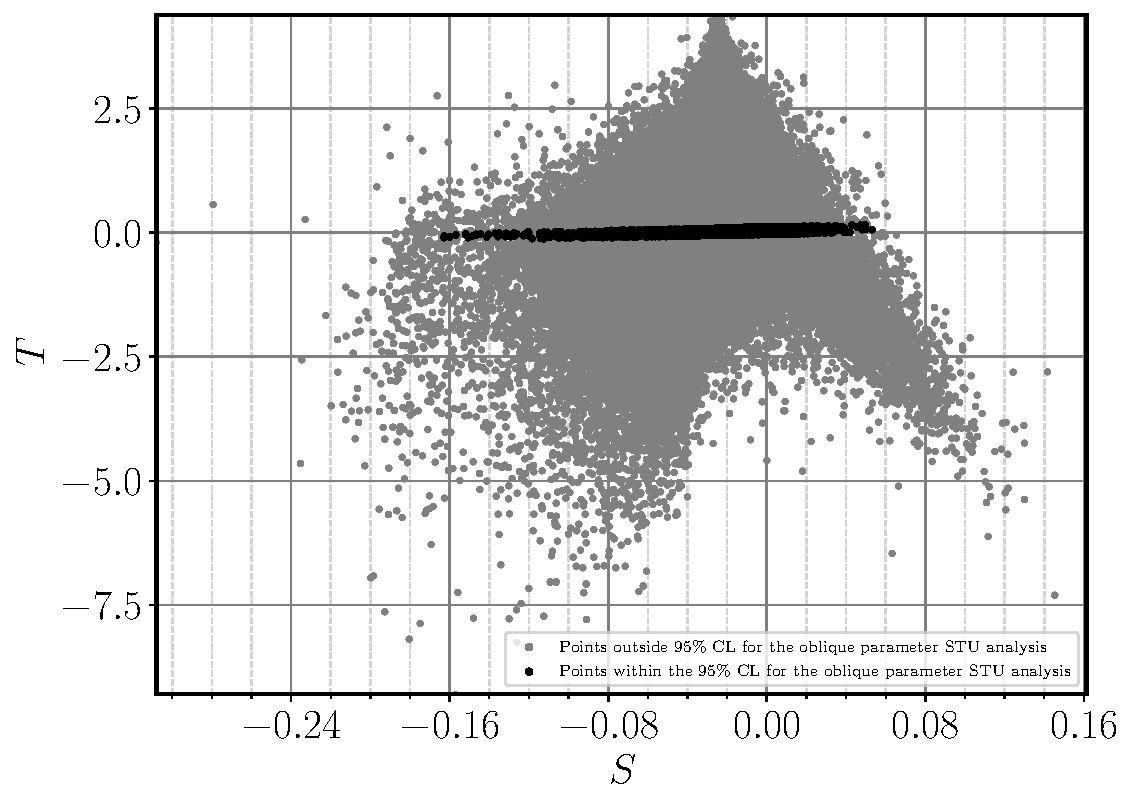
\includegraphics[width=.49\textwidth]{Images/3HDM/EW/EW_S_T_black.pdf}	
	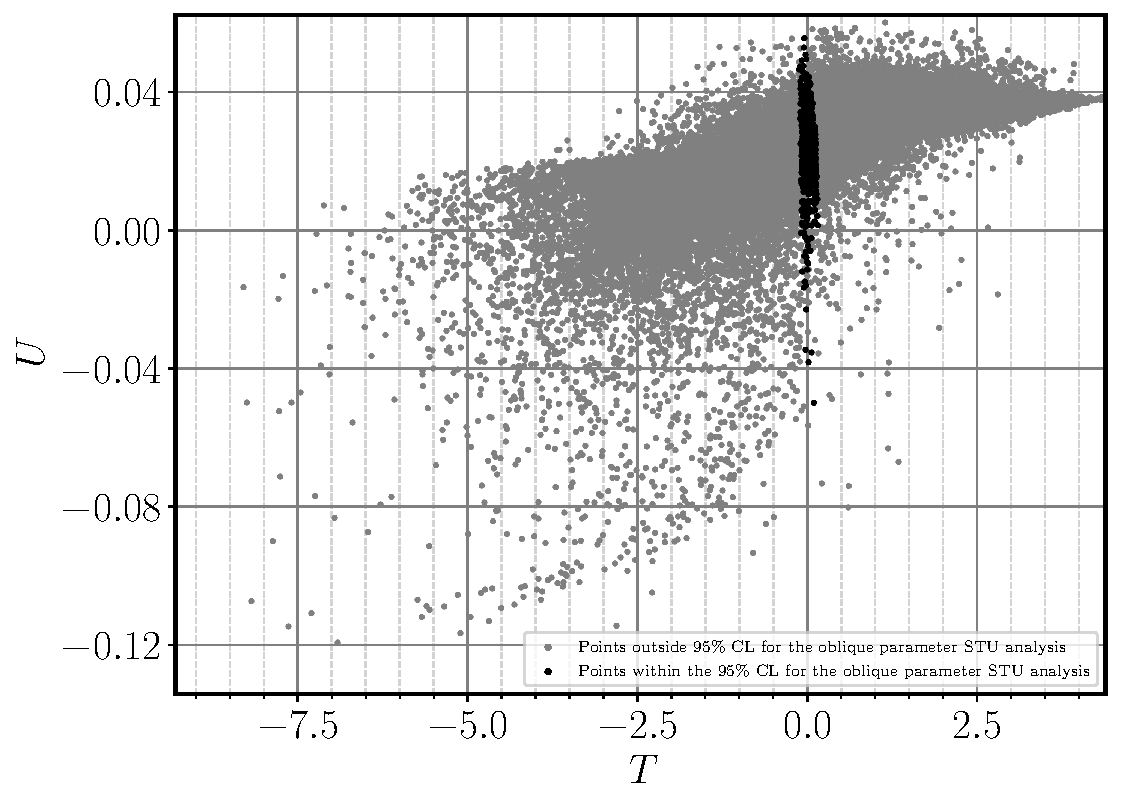
\includegraphics[width=.49\textwidth]{Images/3HDM/EW/EW_T_U_black.pdf}
	\caption{3HDM scatter plots for EW  precision  observables  showing  the ST(left)  and TU(right) planes.  Accepted points lying within a 95\% C.L. ellipsoid of the best fit value are represented in black whereas grey points are excluded.}
	\label{Fig:3HDM_STU}
\end{figure}
%
We can clearly see that NP can have a large effect, most notably on the T variable.
%
As for the B-L-SM the values for $(\Delta S , \Delta T , \Delta U )$ are obtained from \cite{Baak_2012}. All grey points are excluded, while, only the black ones are considered in further analysis.
%
\subsubsection{Direct searches and unitarity constraints}

We show in Fig.\,\ref{fig:H1_A1_Plots} our results from 4 projections of the parameter space involving scalar masses. 
%
Only the green points survive the STU, unitarity and direct searches constraints. Note that, flavour physics observables are not yet considered.  
%
\begin{figure}[!htb]
	\centering
	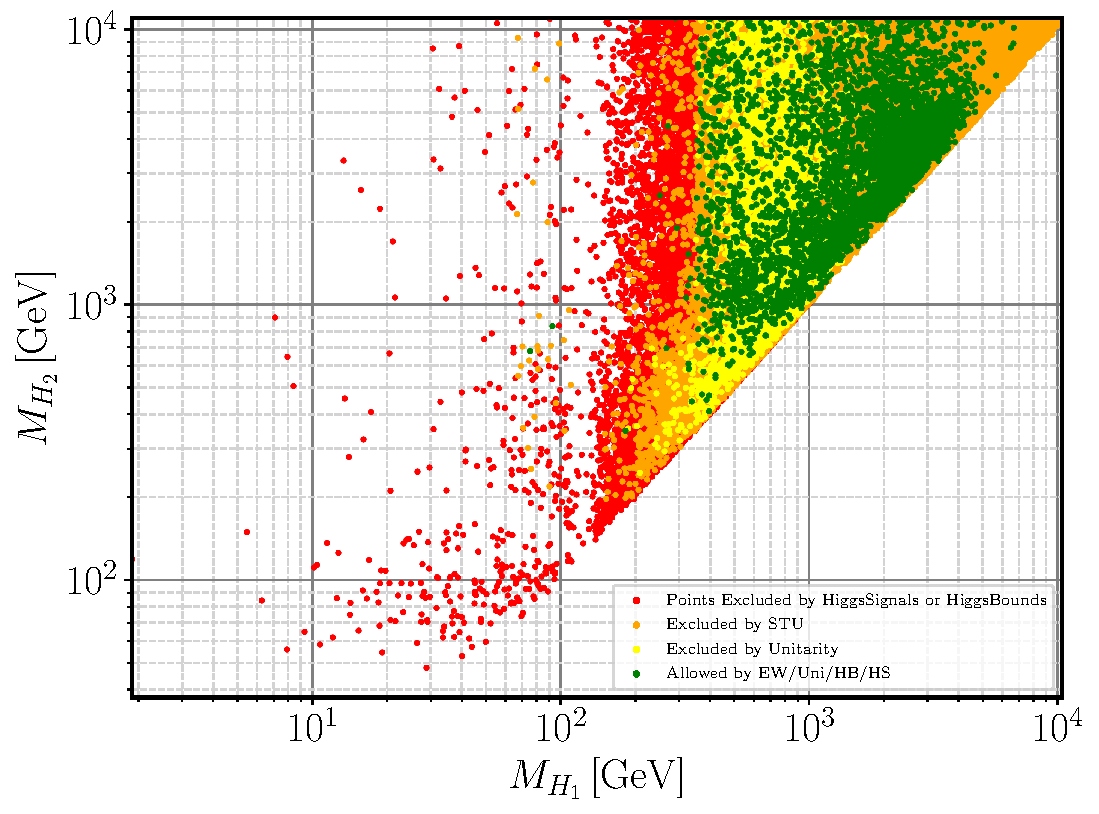
\includegraphics[width=.49\textwidth]{/3HDM/H1_H2.pdf}
	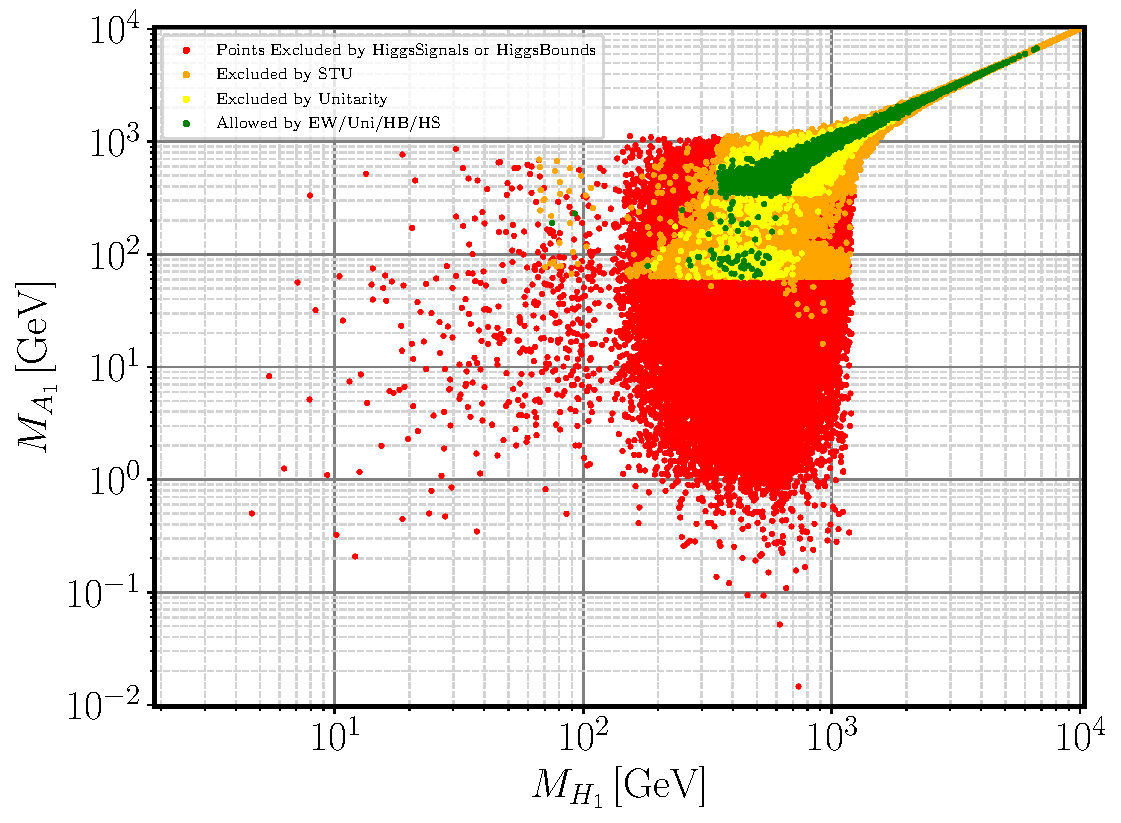
\includegraphics[width=.49\textwidth]{/3HDM/H1_A1.pdf}
	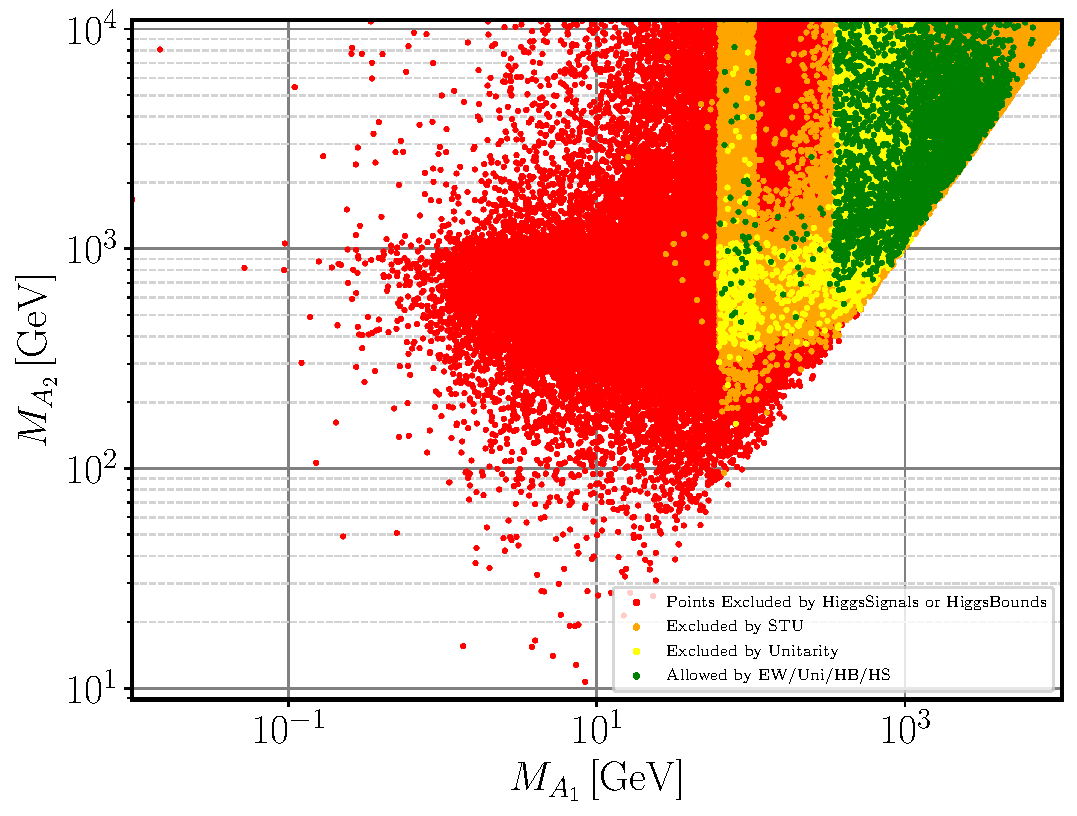
\includegraphics[width=.49\textwidth]{/3HDM/A1_A2.pdf}
	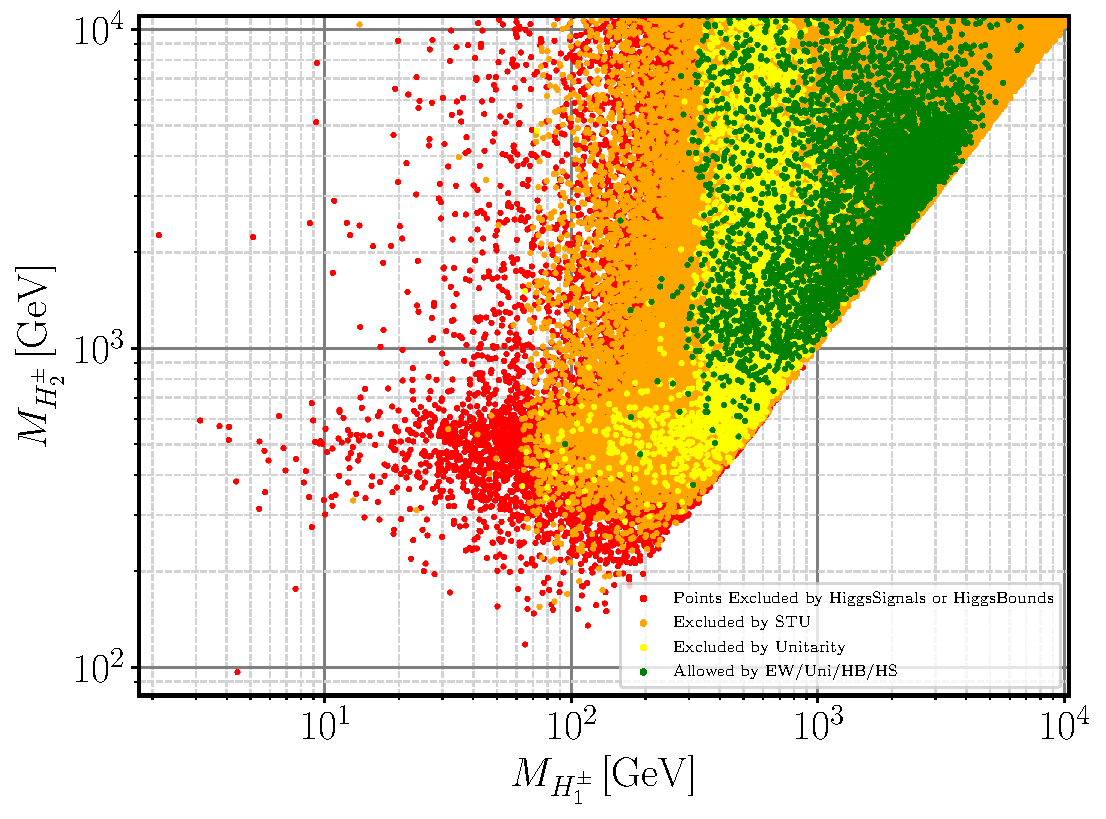
\includegraphics[width=.49\textwidth]{/3HDM/Hc1_Hc2.pdf}
	\caption{Scatter plots of the allowed parameter space. On the upper-left panel we show the masses of the two (non-SM like) $\mathcal{CP}$-even scalars $H_1$ and $H_2$ while in the upper-right we show the relation between the lightest neutral scalar particles ($H_1$ and $A_1$). As for the bottom plots we show the remaining $\mathcal{CP}$-odd and charged scalars and how they are excluded under several constraints. In these plots, red points denote that the HiggsSignals or HiggsBounds tests have failed; yellow points represent scenarios that have failed unitarity constraints; orange points only fail electroweak precision constraints and green ones satisfy all restrictions.}
	\label{fig:H1_A1_Plots}
\end{figure}	

We can observe that direct searches tightly constrain the lightest pseudoscalar and scalar masses.
%
This can be seen on the red regions where, the points that failed HiggsBounds and HiggsSignals are shown. 
%
In particular, we can see that light scalars with masses bellow approximately 60 GeV are ruled out by direct searches. This essentially due to the fact that, for scalars lighter than 125 GeV ($\approx 2 \times 62.5$ GeV) Higgs decays to such scalars becomes kinematically allowed.
%
When we further consider STU and unitarity constraints the allowed regions of the parameter space becomes even more constrained with a small fraction of the originally sampled points in green surviving all tests.
%
Note that, in the bottom-left panel of Fig.\,\ref{fig:H1_A1_Plots}, when the lightest $\mathcal{CP}$-odd scalar approaches the Higgs boson mass the exclusion from direct searches becomes significantly weaker unless the second pseudo scalar also becomes lighter than 200 GeV. 
%
As for all other scalars there does not seem to be a way to reproduce the same effect. 

On the bottom right panel in Fig.\,\ref{fig:H1_A1_Plots} we see that STU limits and unitarity constraints also put strong constraints on how light charged scalars can be. 
%
For instant, while a few green points are seen as light as 100 GeV, the most dense region lies beyond 400 GeV. 

A feature of HiggsBounds is that it also enables us to see the most stringent channel for a given parameter point. 
%
From this we can see that the most restrictive constraints result from the di-photon production and gluon fusion with subsequent decay into light scalars (Limits taken from Refs. \cite{Aad_2014,CMS-PAS-HIG-14-029,Khachatryan_2015}). 

\subsubsection{Flavour Observables }

Let us now study the effect of QFV observables on the sampled points. 
%
First, by analysing our models predictions and comparing with experimental bounds, this can be seen in  Fig.\,\ref{fig:3HDM_Flavour} where we show the most representative examples.
%
The first thing to highlight is that the allowed region for $\varepsilon_K/\varepsilon_{K_{SM}}$ and ${\Delta M_s}/{\Delta M_{s_{SM}} }$ appears to be rather small.
 %
 This follows from the fact that the ${\textrm{BR} ( \textrm{B} \rightarrow X_s \gamma)}/{\textrm{BR}_{SM} ( \textrm{B} \rightarrow X_s \gamma )}$ and ${\Delta M_s}/{\Delta M_{s_{SM}} }$ observables are very tightly constrained and are the most sensitive ones. 
 %
\begin{figure}[!htb]
	\centering
	%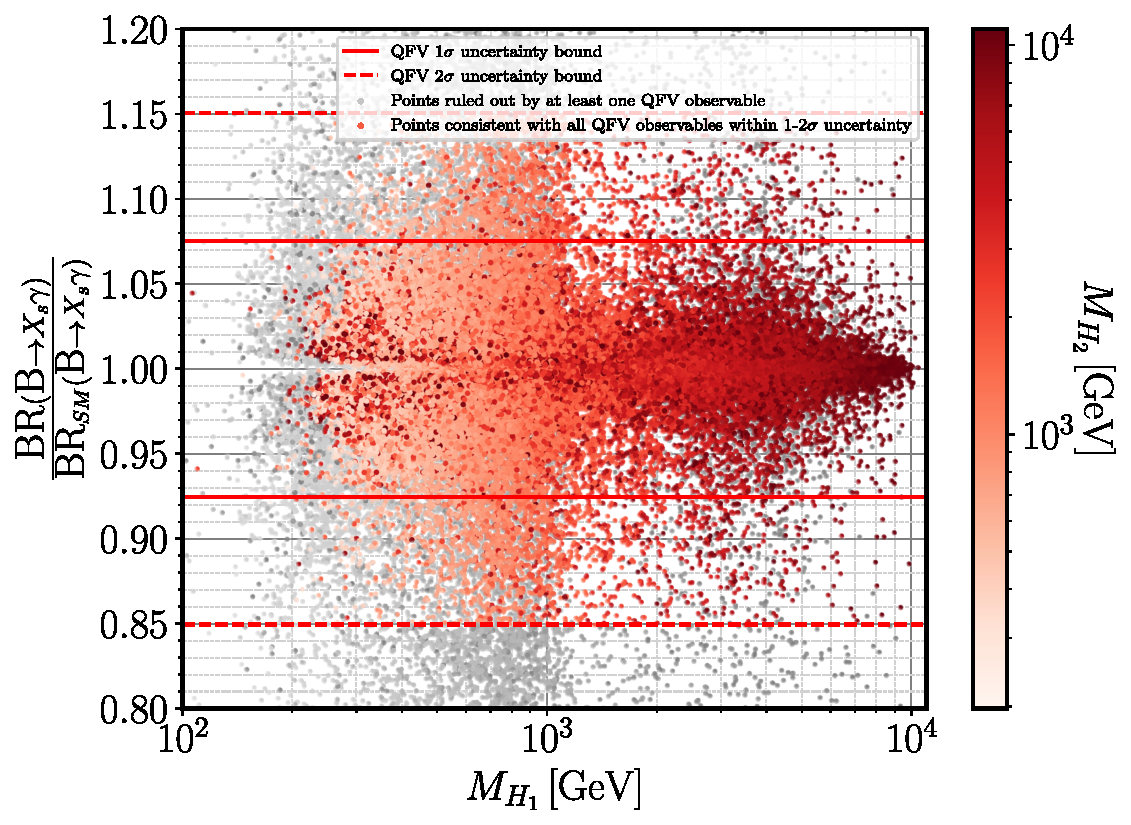
\includegraphics[width=.49\textwidth]{Images/3HDM/Reds/Xsgamma_H1_H2_2.pdf}
	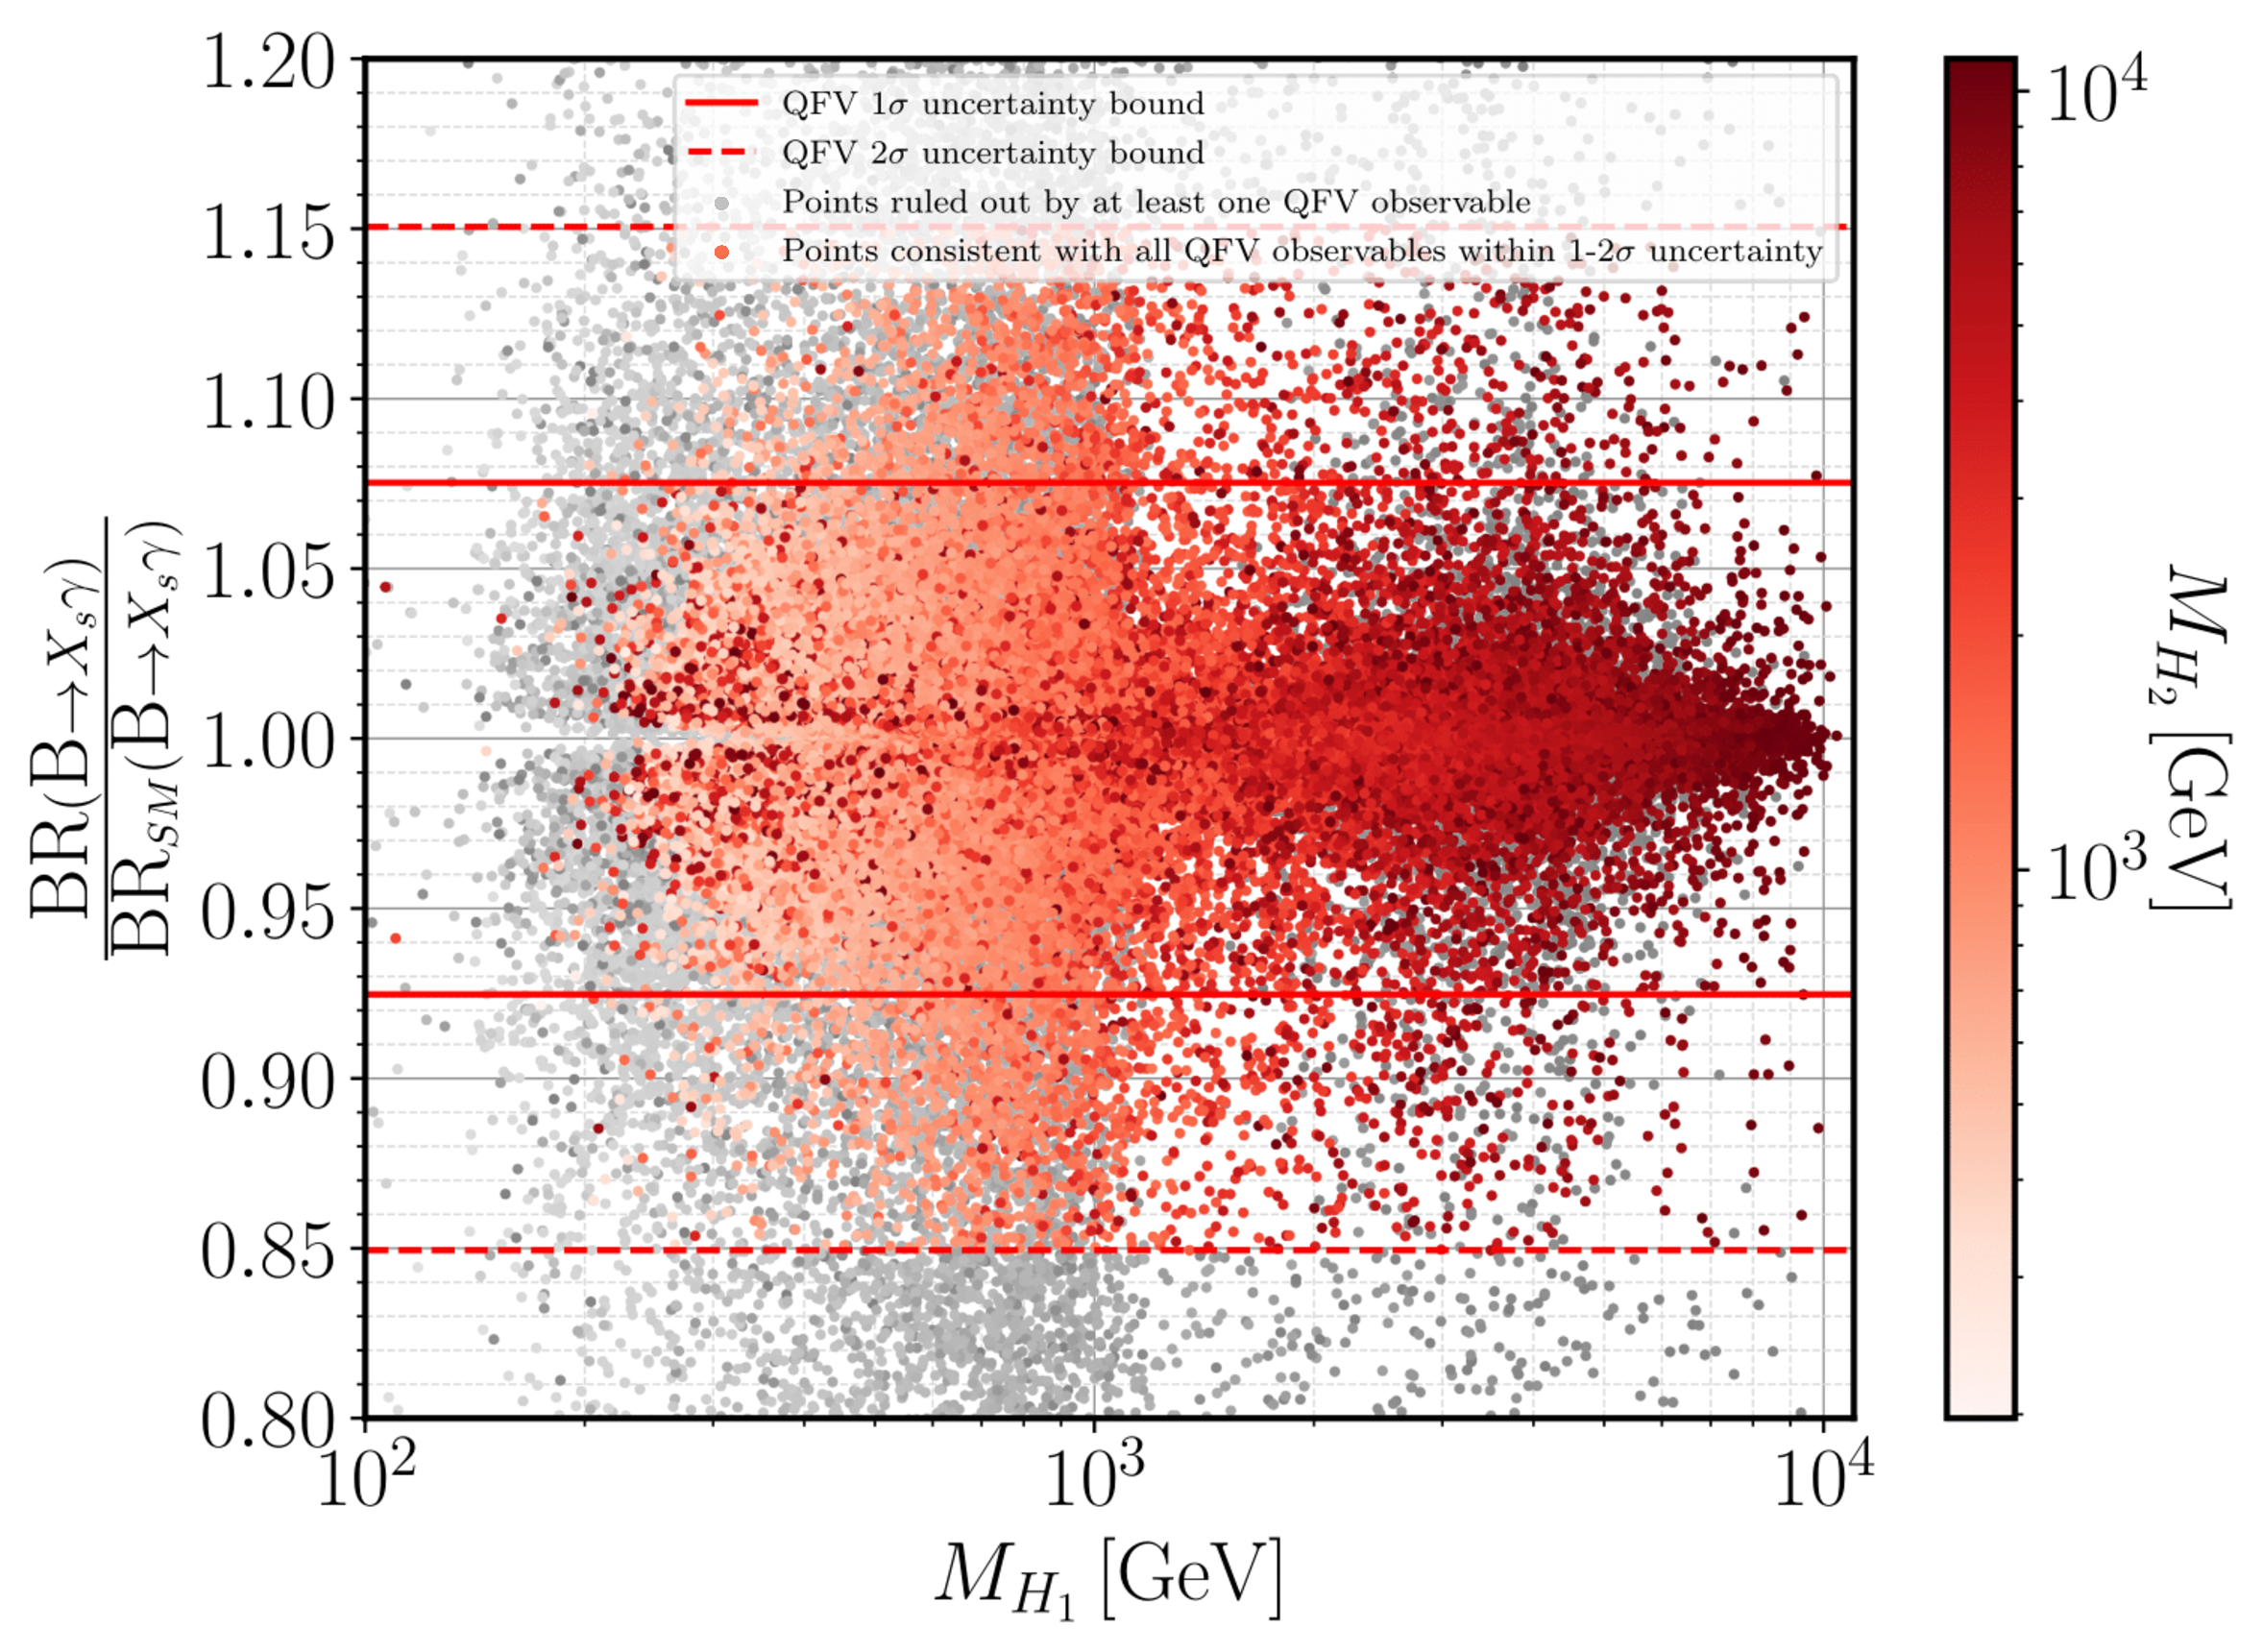
\includegraphics[width=.49\textwidth]{Images/fix_2.pdf}
	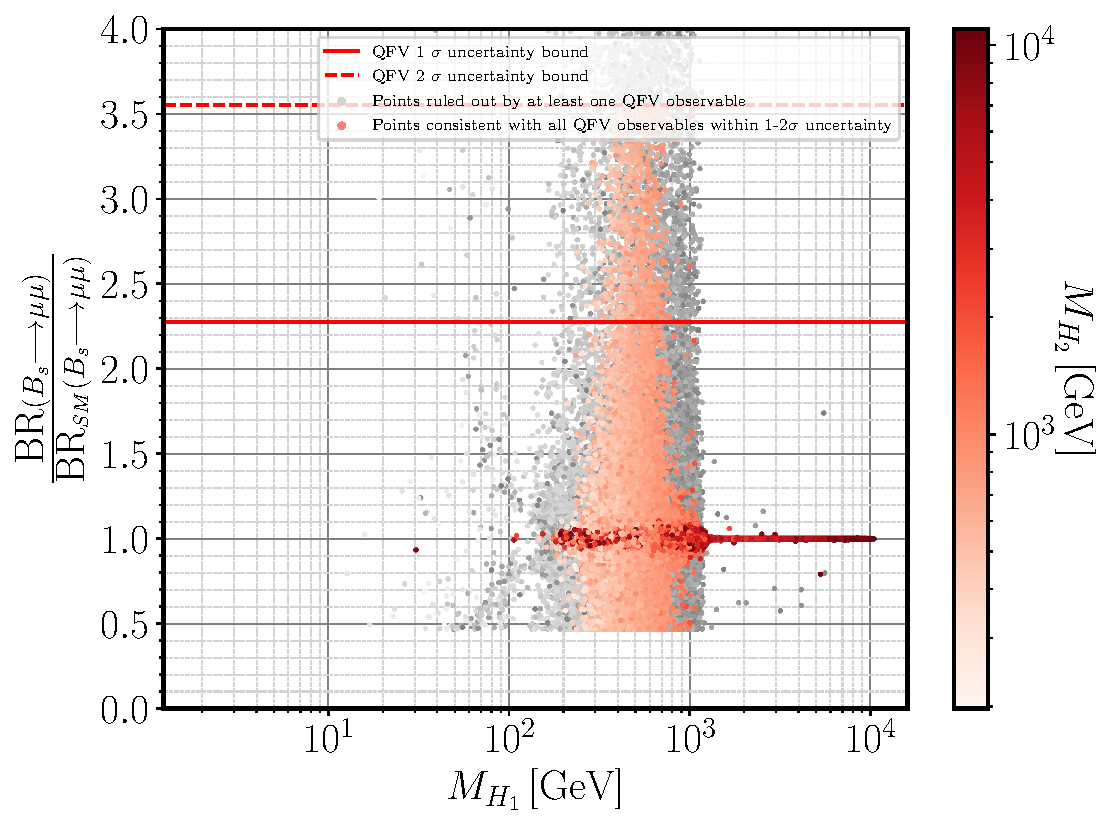
\includegraphics[width=.49\textwidth]{Images/3HDM/Reds/Bsmumu_H1_H2.pdf}
	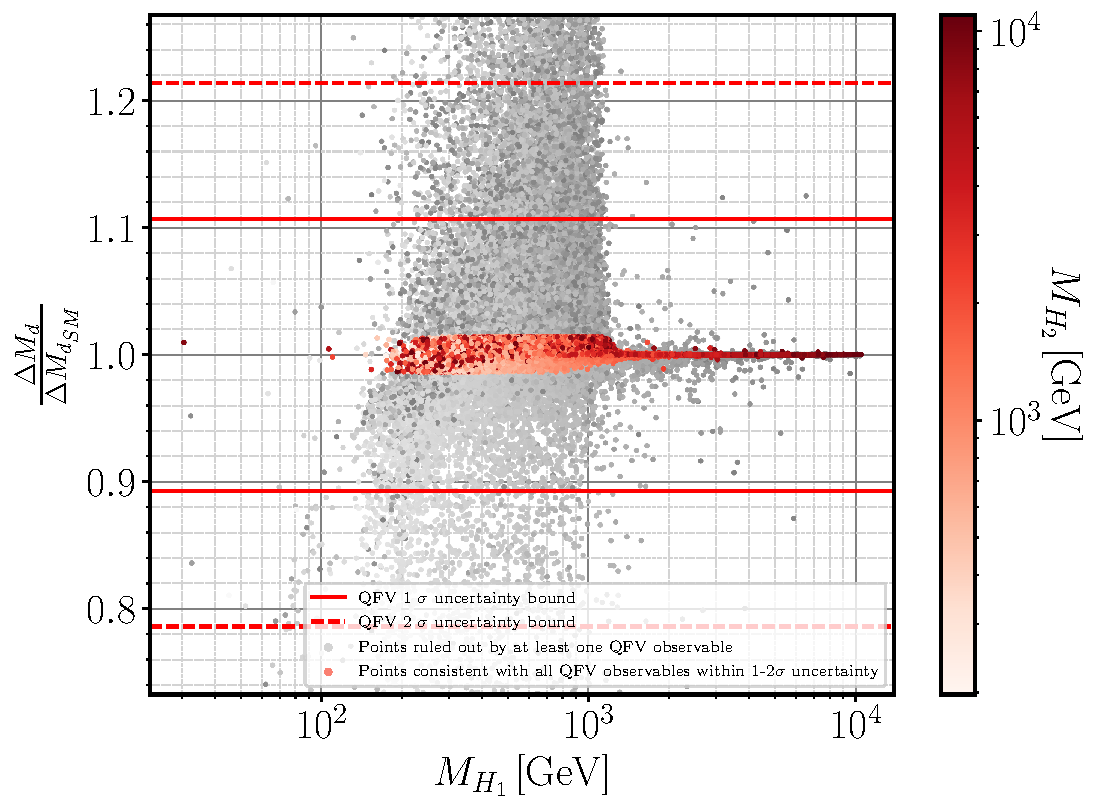
\includegraphics[width=.49\textwidth]{Images/3HDM/Reds/DeltaMd_H1_H2.pdf}
	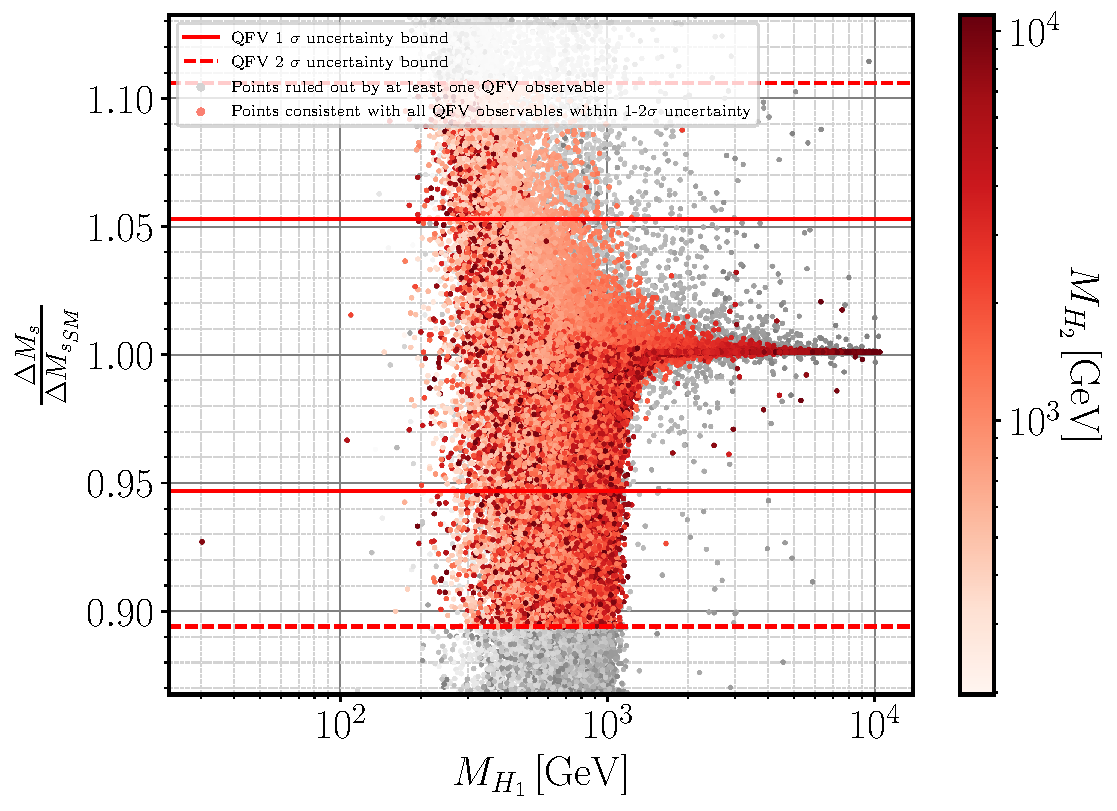
\includegraphics[width=.49\textwidth]{Images/3HDM/Reds/DeltaMs_H1_H2.pdf}
	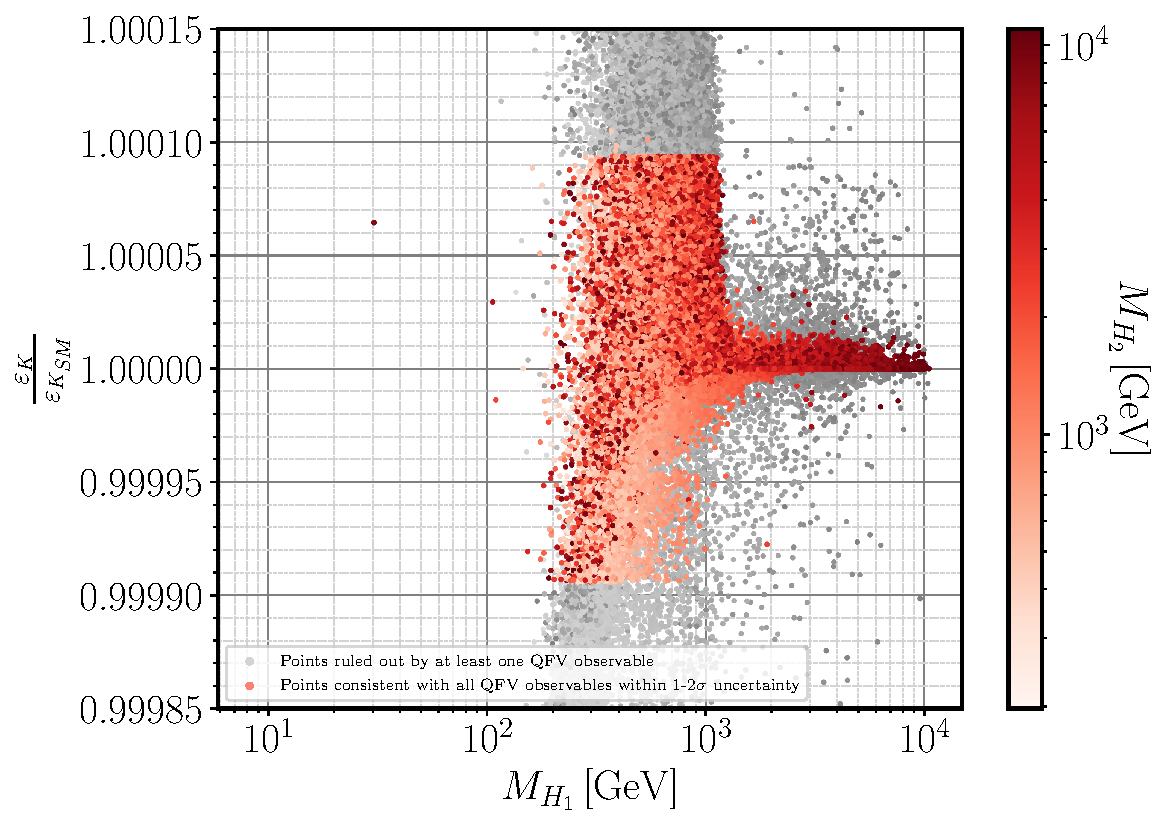
\includegraphics[width=.49\textwidth]{Images/3HDM/Reds/Eps_K_H1_H2_Centered.pdf}
	\caption{ Scatter plot of the estimated QFV observables normalized to the SM values versus the lightest scalar Higgs. The grey points in all plots represent a point that would be outside the 2 $\sigma$ bound for any of the observables while in a red color scale we show the second $\mathcal{CP}$-even neutral scalar mass for those scenarios where every single QFV observable is within their 2 $\sigma$ uncertainty band.}
	\label{fig:3HDM_Flavour}
\end{figure}
%
Indeed, when we combine all QFV observables, the model prediction for the allowed region in the $\Delta M_d$ and $\epsilon_k$, red points, lies well bellow their 1 $\sigma$ uncertainty and very close to the SM value. 
%
The same is not verified for $\textrm{B} \rightarrow X_s \gamma$,$\textrm{B}_s \rightarrow \mu \mu$, $\Delta M_s$ for the SM up to 2 $\sigma$ it is also without surprise that we see deviations from the SM fading away for larger scalar masses. 
%
The next step is to combine QFV observables with the remaining constraints previously discussed. Our results are shown in Fig.\,\ref{fig:3HDM_Flavour_PT}. 
%
Here we clearly see that there is a central region where the points comply with all constraints.
%
In particular, it is interesting to note that the green points that have also survived STU, unitarity and direct searches constraints, tend to pile close to the center of the cloud of points instead of randomly scatter. This suggests that the BGL suppression is more effective for scenarios that are consistent with such theoretical and experimental constraints. 
%
This is a very important conclusion we take from our model. Through the stabilization of the 3HDM by the flavour symmetry all QFV observables are kept under significant deviation for all the viable mass spectrum.  

\begin{figure}[!htb]
	\centering
	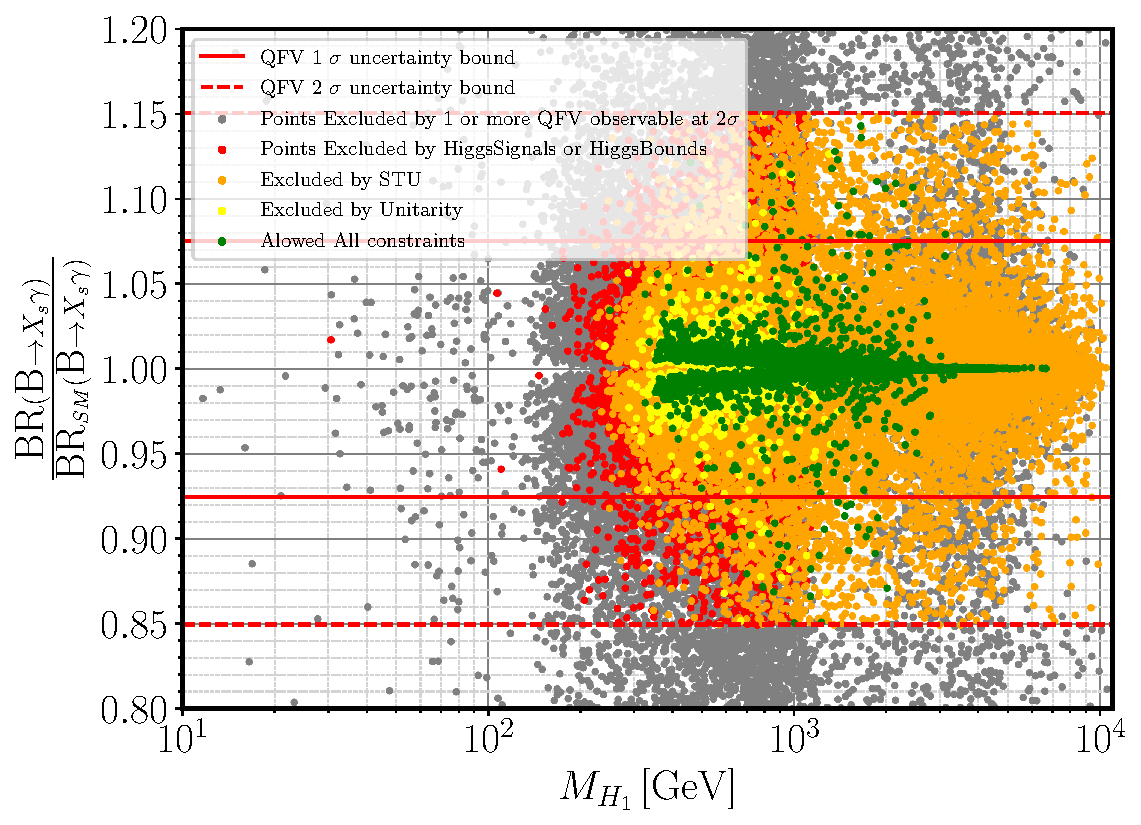
\includegraphics[width=.49\textwidth]{Images/3HDM/PT_Folder/XsGamma_H1.pdf}
	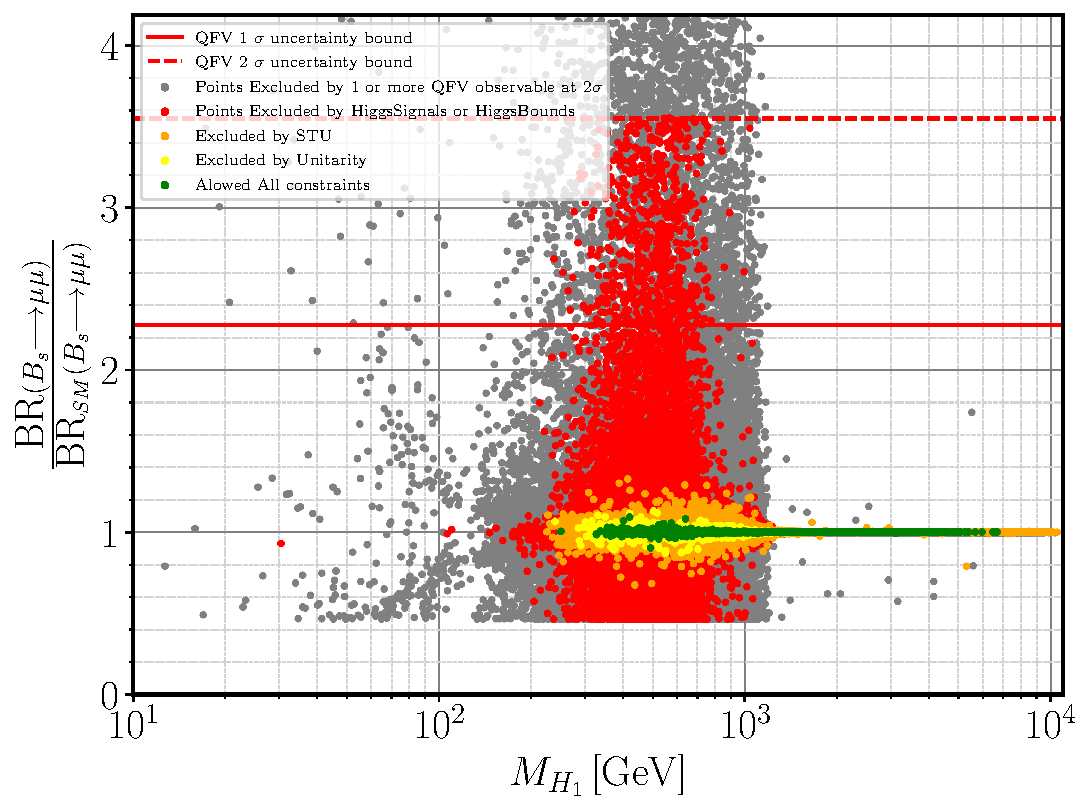
\includegraphics[width=.49\textwidth]{Images/3HDM/PT_Folder/Bsmumu_H1.pdf}
	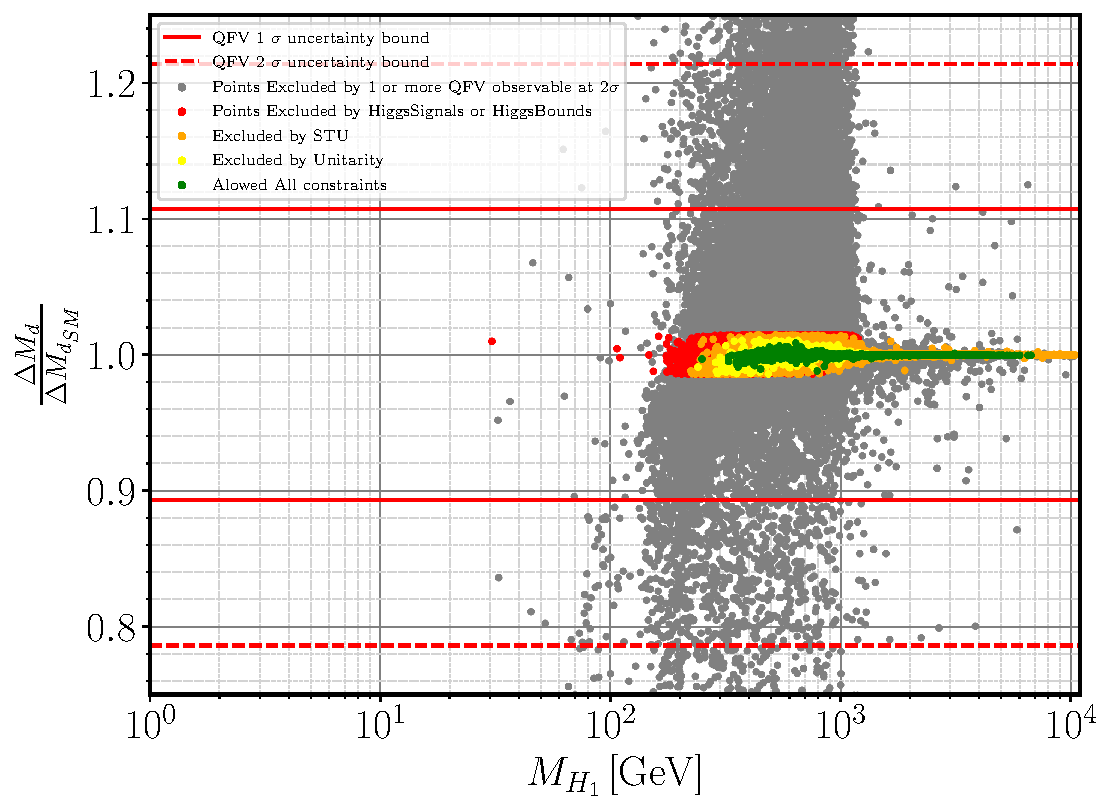
\includegraphics[width=.49\textwidth]{Images/3HDM/PT_Folder/Delta_Md_H1.pdf}
	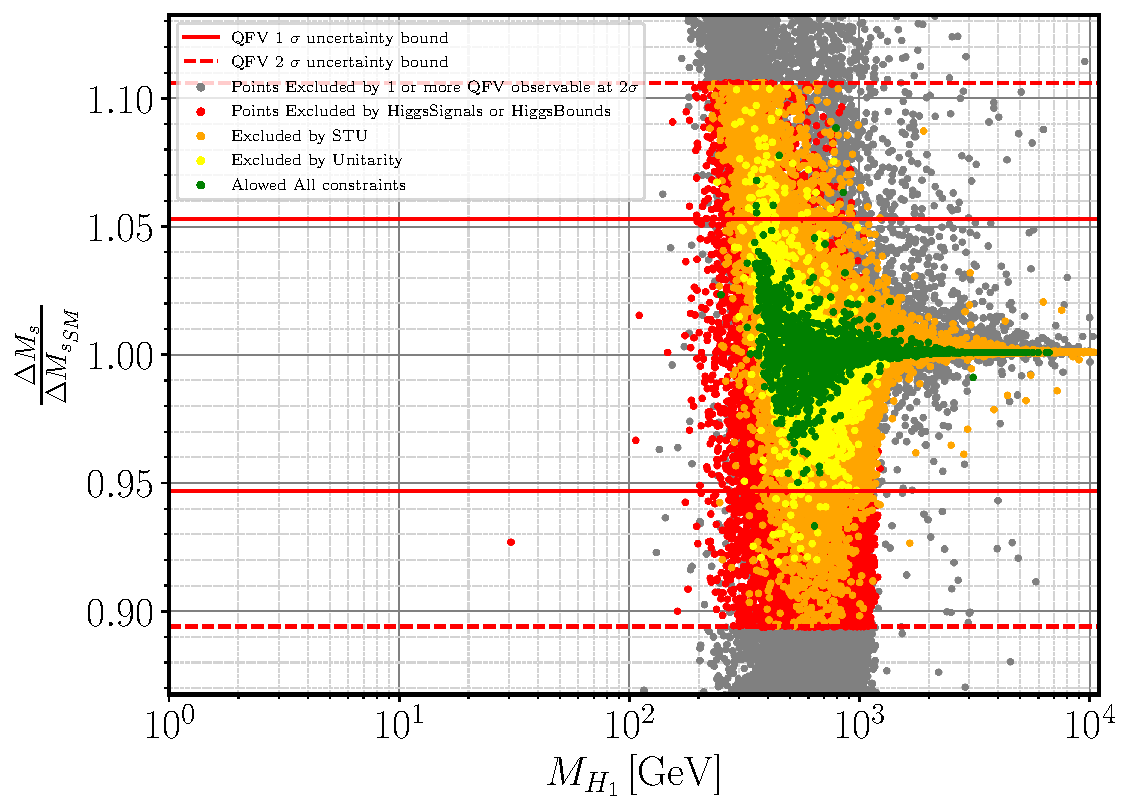
\includegraphics[width=.49\textwidth]{Images/3HDM/PT_Folder/Delta_Ms_H1.pdf}
	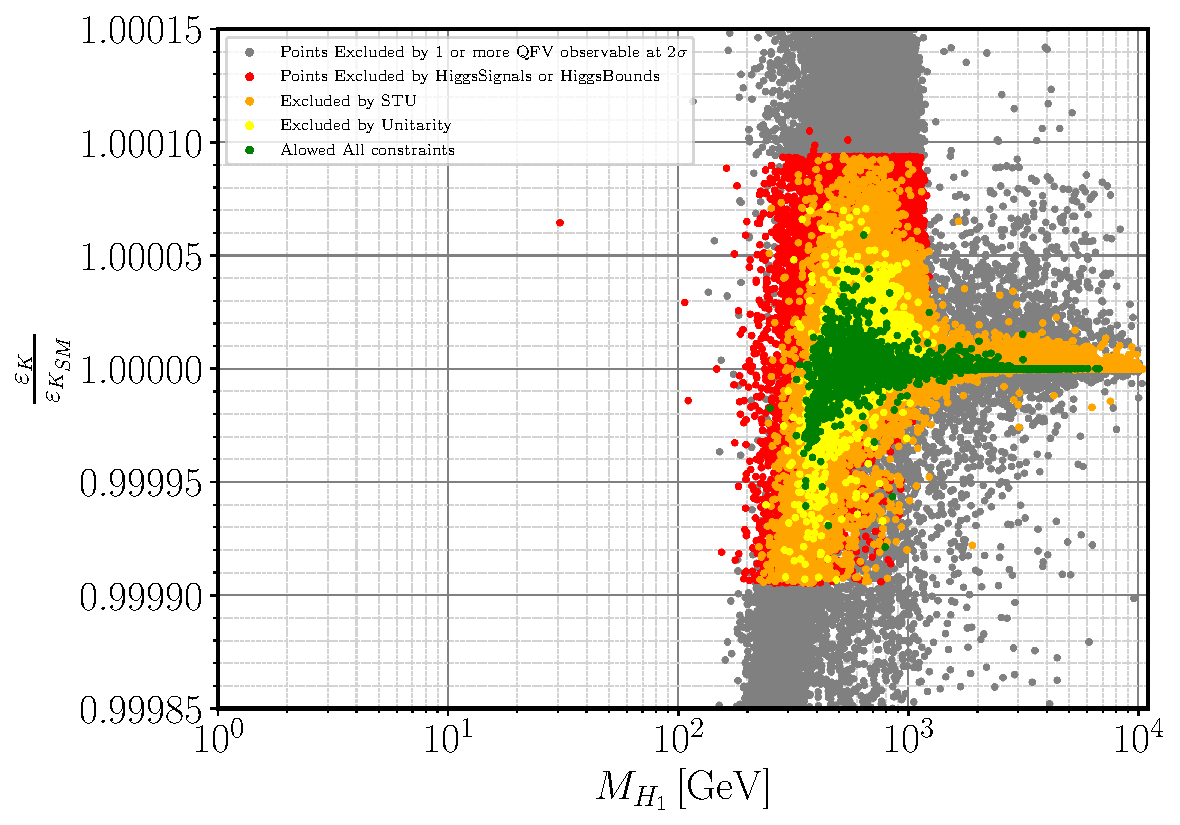
\includegraphics[width=.49\textwidth]{Images/3HDM/Reds/Eps_K_H1_Thighter_Centered.pdf}
	\caption{ Scatter plot of the estimated QFV observables normalized to SM values overlapped all other experimental and theoretical constraints.} 
	\label{fig:3HDM_Flavour_PT}
\end{figure}

For completeness, we select six possible benchmark points, showing them in Tab.\,\ref{Tab:BadTable}.
%
As we can see from these values, several combinations of light scalars are still allowed in the model. This opens up the possibility for dedicated searches at the LHC and one can also have a significant impact in explaining possible deviations in flavour physics.
%
It is also very remarkable that to note that the lightest pseudoscalar is allowed to be lighter than the SMs Higgs boson with a mass as low as 87 GeV. Furthermore the benchmark that minimize $m_A$ push all other scalar masses down. For instance the heaviest charged and neutral are smaller than 470 GeV. We would like to point out that this is a particularly appealing scenario for the LHC run III.  

\begin{table}[!htb]
	\centering
	\begin{tabular}{c|c|c|c|c|c|c|}
		\cline{2-7} 
		& $m_{H_1}$ & $m_{H_2}$ & $m_{A_1}$ & $m_{A_2}$ & $m_{H^\pm_1}$ & $m_{H^\pm_2}$ \\ \hline
		\multicolumn{1}{|c|}{\multirow{2}{*}{Lightest $H_1$}}     & 251 & 2488 & 247 & 2616 & 157 & 2510  \\ \cline{2-7} 
		\multicolumn{1}{|c|}{}                                    & 327 & 1528 & 359 & 1616 & 229 & 1561  \\ \hline
		\multicolumn{1}{|c|}{\multirow{2}{*}{Lightest $A_1$}}     & 386 & 452  & 87  & 467 & 189  & 466  \\ \cline{2-7} 
		\multicolumn{1}{|c|}{}                                    & 337 & 446  & 100 & 395 & 311  & 374  \\ \hline
		\multicolumn{1}{|c|}{\multirow{2}{*}{Lightest $H^\pm_1$}} & 251 & 2488 & 247 & 2616 & 157 & 2510 \\ \cline{2-7} 
		\multicolumn{1}{|c|}{}                                    & 398 & 1314 & 282 & 1525 & 173 & 1314 \\ \hline
	\end{tabular}
	\caption{A selection of six benchmark points. All masses are given in GeV. These correspond to the lightest scalars found that respect all QFV and scalar sector constraints.}
	\label{Tab:BadTable}
\end{table}

\subsubsection{Fine-Tuning analysis}

We have mentioned that in some NHDMs flavour changing effects can only be small if one relies on fine-tuning model parameters. 
%
However, scanning randomness combined with a large amount of data could have found a synchronicity where flavour observables are fine-tuned by accident. 
%
To check if this phenomena was present, all points were recalculated with a slight variation of masses through a 1\% change on the soft breaking terms, $\mu_{13}$, $\mu_{23}$ and $\mu_{21}$. 
%
Such a mass variation is expected to lead to variation of the flavour decay amplitudes. 
%
With this exercise we expect to show that there is no abruptly large variation of masses or QFV observables as to show no fine-tuning is present.
% 
The results can be seen in Fig\,\ref{fig:3HDM_Fine_Tunning}, where we show two representative examples. Indeed we see that 1\% variation on the soft parameters yields a smaller variation in $\textrm{B} \rightarrow X_s \gamma$  and ${\Delta M_s}$ while it produces almost no effect on the value of $\epsilon_k$. Therefore we consider that our model does indeed keep FCNCs under control by means of the BGL-like symmetry rather than by accidental cancellations. 

\begin{figure}[htb!]
\centering
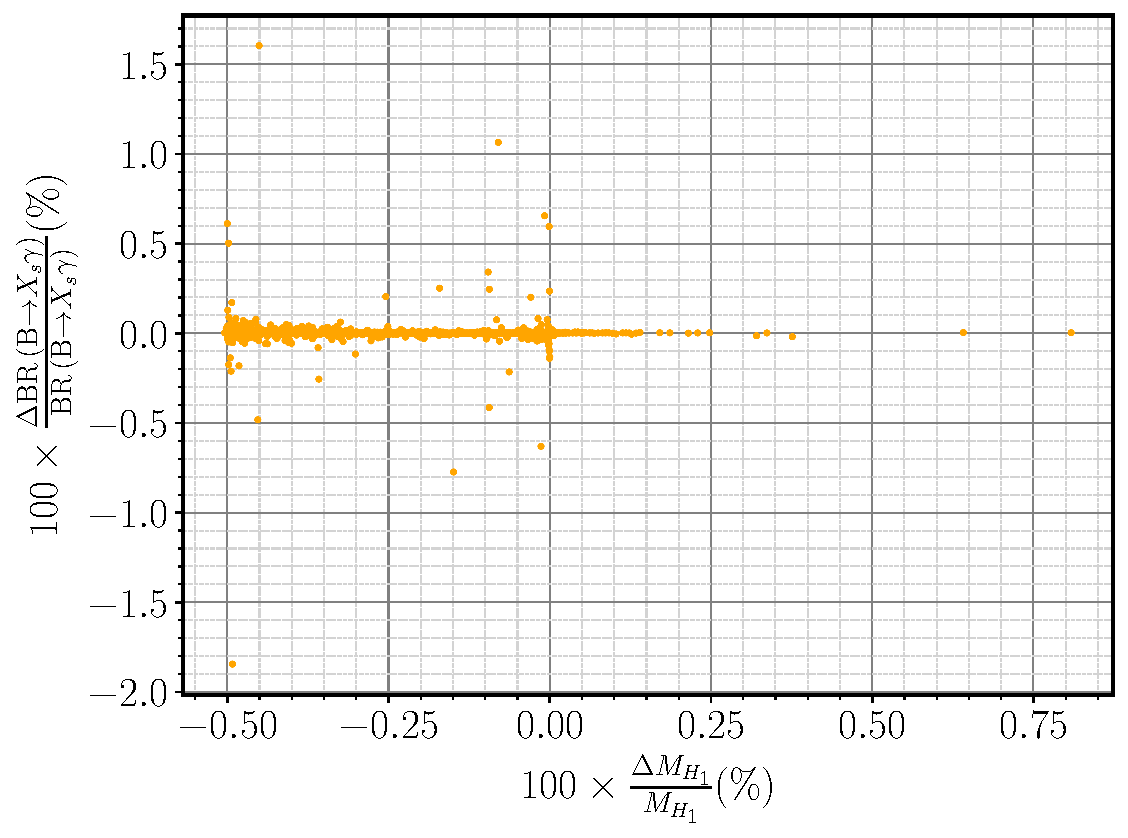
\includegraphics[width=.49\textwidth]{Images/3HDM/Fine_Tuning/Xsgamma_H1.pdf}
%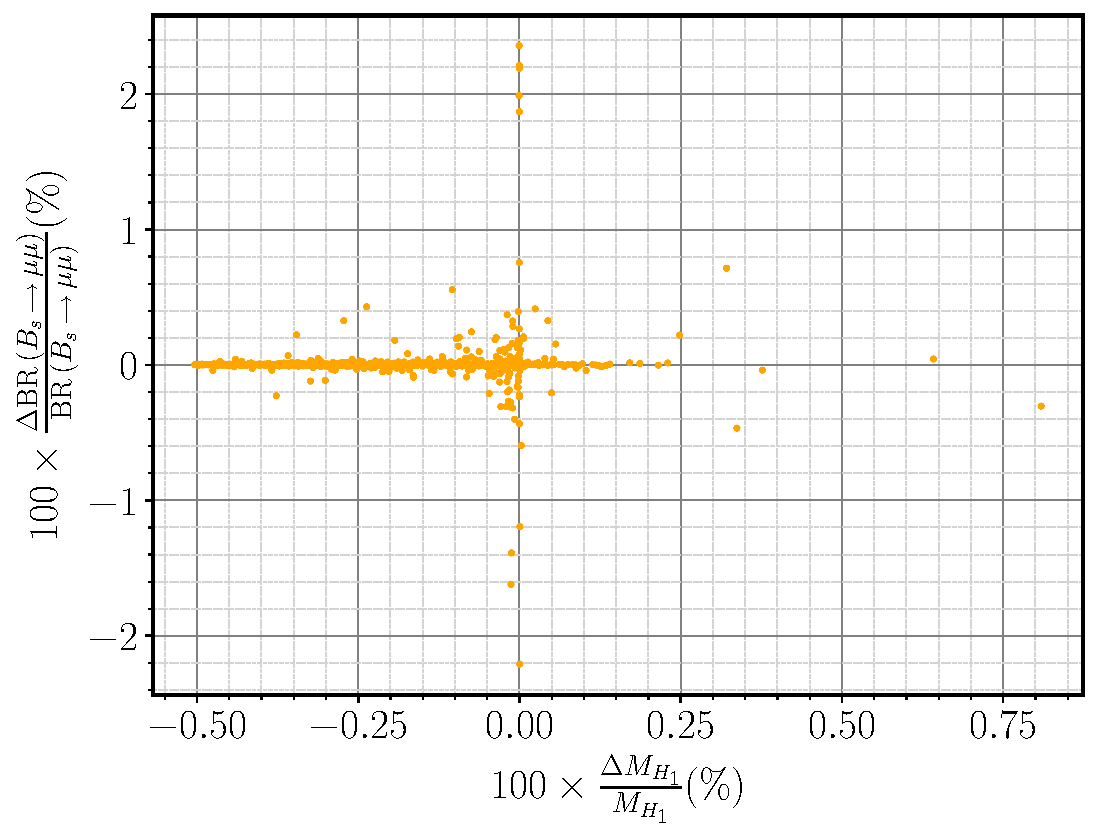
\includegraphics[width=.49\textwidth]{Images/3HDM/Fine_Tuning/Bsmumu_H1.pdf}
%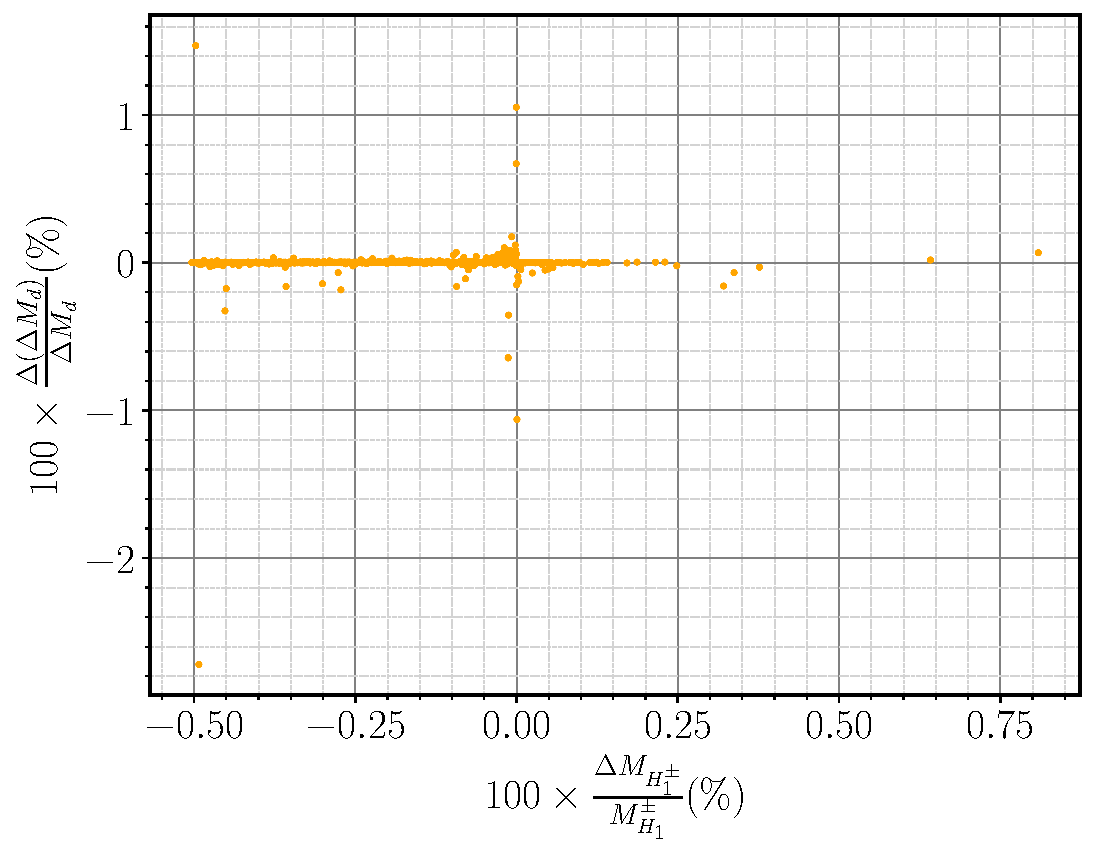
\includegraphics[width=.49\textwidth]{Images/3HDM/Fine_Tuning/DeltaMd_H1.pdf}
\includegraphics[width=.49\textwidth]{Images/3HDM/Fine_Tuning/DeltaMs_H1.pdf}
\includegraphics[width=.49\textwidth]{Images/3HDM/Fine_Tuning/eps_K_H1.pdf}
\caption{Relative mass and QFV observable changes with the increase of 1\% in all soft breaking terms}
\label{fig:3HDM_Fine_Tunning}
\end{figure}	

Last but not least, we have computed the cross section for the gluon-gluon production of the lightest $\mathcal{CP}$-even and odd scalars for a center of mass energy of 13 TeV as shown in Fig.\,\ref{Generic_3HDM_Result_Label}. 
%
The exclusion bands for the gluon fusion production of a pseudoscalar, scalar and associated production with a bottom pair were taken from Fig. 7 of the CMS paper \cite{Sirunyan_2018}. 
% 
To do so we have used \texttt{MadGraph5\_aMC@NLO 2.6.2} in our chain of codes. 
% 
These plots emphasize the relevance of requiring agreement with all QFV observables. 
% 
In fact fact, only blue points survive such constraints while grey ones, deviate by more than 2$\sigma$ for at least one QFV observable. 
%
As expected, the signal strength becomes weaker for larger masses. In particular we notice the drop around $m_{A_1}$ and $m_{H_1}$ around 375 GeV, that is twice the top mass. As such the decay channels $A_1 \to \bar{t}t$ and $H_1 \to \bar{t}t$ become kinematically allowed tending to reduce the $A_1 \to \bar{\tau} \tau$ and $H_1 \to \bar{\tau} \tau$ branching fractions.
%
Finally notice that there are a number of points for lower masses which can almost be probed by the current CMS bounds. For completeness sake we also show the di-tau channel in its associated production with a bottom quark pair. Despite a slightly smaller cross-section we observe the same features. Therefore we can say that our BGL-like 3HDM is not far from being probed by current data and, before the end of run III parts of its the parameter space can already be excluded, or lead to discovery by extra scalar searches. 

%
\begin{figure}[htb!]
	\centering
	\includegraphics[width=.49\textwidth]{Images/3HDM/Xsec/Xsec_1_Grey_tight.pdf}	\includegraphics[width=.49\textwidth]{Images/3HDM/Xsec/Xsec_2_Colourful_tight.pdf}
	\includegraphics[width=.49\textwidth]{Images/3HDM/Xsec/Xsec_3_Grey_Thight.pdf}
	\caption{Scatter plots showing gluon-fusion production of $\mathcal{CP}$-even scalars (top-left) and pseudo-scalar (top-right) and scalar production in association with a bottom quark pair. Grey points represent those that are excluded by at least one QFV observable. On the other hand, blue points are allowed by all constraints, namely the QFV ones.}
	\label{Generic_3HDM_Result_Label}
\end{figure}	
%
%With these plots we can see that not only the region is clearly all bellow detection validating HiggsBounds, as we can also see there is space left to be probed at new collider experiments, both near and far from detection. 
%
This means we could be close to a new signature detection at the LHC through gluon fusion. If such a signature is discovered then we can move to examine how this would impact QFV deviations and further pin-point the validity of multiple Higgs doublets.  

\chapter{Conclusions}
\label{ch:Conclusions}

To summarize, in this thesis we have performed a detailed phenomenological analysis of the minimal $\U{B-L}$ extension of the Standard Model, known as the B-L-SM, and of a BGL-like 3HDM with a $\mathrm{U(1)} \times \mathbb{Z}_2$ symmetry. 
%
This phenomenological analysis was produced by a set of tools developed as to be easily adaptable to fit new models. 

In the B-L-SM (chapter \ref{Chap:B-L-SM_Model}) we have performed a detailed phenomenological analysis confronting the model with the most recent experimental bounds from the direct $Z^\prime$ boson and next-to-lightest Higgs state searches at the LHC, as well as with the LEP constraints on four-fermion contact interactions.

We have studied the correlations of the $Z^\prime$ production cross section times the branching ratio 
into a pair of light leptons versus the physical parameters of the model. In particular, we have found 
that the muon $(g-2)_{\mu}$ observable dominated by $Z^\prime$ loop contributions is maximized 
for $m_{Z^\prime}$ between $6.3$ and $6.5~\ro{TeV}$. As one of the main results of our analysis, we have found phenomenologically consistent model parameter space regions that simultaneously fit the exclusion limits from direct $Z^\prime$ searches and maximize the muon $(g-2)_\mu$ contribution to a value of $8.9 \times 10^{-12}$. This represents a marginal or no improvement in comparison to the SM prediction.

While a confirmation of the currently observed anomaly with a smaller error can 
become rather exciting news, a more pessimistic scenario when the discrepancy either disappears or partially reduces, would reinforce the significance of our result and offer a motivation for future $Z'$ searches at the LHC in the $5-7~\mathrm{TeV}$ domain. 

Another important result resides in the fact that an increasingly heavy $Z'$ boson also pushes up 
the mass of the second Higgs boson. Therefore, the hypothetical observation of such new physics 
states as a scalar or a vector boson would pose stringent constraints on the B-L-SM.
For completeness, we have also estimated the dominant contribution from the Barr-Zee type 
two-loop corrections and found a relatively small effect.

%%%%%% 

%As for the 3HDM component of our work in this these seen in  Chapter\,\ref{ch:3HDM}. 
%
We studied the phenomenological consistency of a BGL-like 3HDM model. We have identified regions where both flavour and scalar sector physics are within experimental bounds including, like in the B-L-SM, EW precision observables and direct detection constraints.  
%
This has enabled us to narrow down the allowed  the parameter space regions which simultaneously fit all theoretical and experimental constraints. %the exclusion limits from direct scalar searches and flavour constraints 
We have also discussed the possibility of probing the model in the gluon fusion channel. 
%
In particular we have observed that the BGL-like 3HDM offers the possibility for lighter than conventionally allowed non-standard scalars, at the reach of the LHC III.
%
Our analysis determined the most sensitive flavour violation channels, and has revealed that the BGL-like mechanism induced by the $\mathrm{U(1)}\times\mathbb{Z}_2$ flavour symmetry is indeed responsible for the suppression of FCNCs rather than any accidental fine-tuning. Let us also comment that further deviations in these flavour observables might be a pathway to indirectly discover new scalars (or other exotic particles) mediating these phenomena.  
%
For the case of our 3HDM, the appropriate channels to peer into this are the B meson oscillations and B meson decays.% for this type of 3HDM.

However, a key take away from our results is that the most stringent constraints on the model are not the flavour observables but the Higgs physics limits. 
%
Notice that, a natural extension of this work is to relax the exact alignment limit, which is left for future work. 
%
Note, although we use conventional methods to perform our analysis, some recent studies have incorporated new strategies such as machine learning. Similarly to what was done by our colleagues in \cite{freitas2020phenomenology}, these modern techniques promise to greatly increase the efficiency of similar studies, and are a plan for future discussions. 
%
%Unfortunately this wasn't accomplished in this work due to the exceptional setbacks. A feature of this year, that affected partially the quality of the work. 
%
These machine learning routines could drastically increase the speed at which these simulations are made, but also facilitate the discovery of new parameter space regions that normal random scans would take a long time to generate. 

\bibliographystyle{IEEEtran}
%\bibliography{plain}
\bibliography{bib.bib,bib_blsm.bib,bib_blsm_2}

\endgroup
\end{document}

